\documentclass[12pt,letter]{article}
\usepackage{../downey_format}

\begin{document}
	
	% set the section number, along with figure and equation numbers
	\setcounter{section}{4}	
	\setcounter{figure}{0}   
	\renewcommand\thefigure{\thesection.\arabic{figure}}
	\setcounter{equation}{0}   
	\renewcommand\theequation{\thesection.\arabic{equation}}
	
		\section{Multiple Degree-of-freedom Systems}
	
	
	
	Until now we have only considered and modeled systems that can require one coordinate system to describe their motion. In this chapter, we will develop the mathematical tools required to model multiple degree-of-freedom systems that require multiple independent coordinates to describe their motion. As before, the equations that describe the motion of rigid bodies in space are developed from Newton's second law of motion. However, unlike before, there exists an independent equation for each body in motion. These equations are therefore coupled by the system and are often expressed in matrix notation such that the mass, damping, and stiffness matrices are easily defined. 
	
	
	
	
	\begin{review}
	\textbf{Linear Algebra}
	
	\noindent Linear algebra allows for the efficient solving of these coupled equations. In this text, matrices are expressed as bold capital letters ($\textbf{X}$), vectors are denoted with an arrow ($\vec{x}$), and scalars/variables with italic letters ($x$). However, given the range of notation needed, it is not always possible to strictly follow this formulation.
	
	The dot product allows us to multiply matrices and is defined as:
	\begin{eqnarray}
	  \begin{bmatrix} a & b \\ c & d \end{bmatrix}\begin{bmatrix} e \\  f \end{bmatrix} = \begin{bmatrix} ae+bf \\ ce + df \end{bmatrix}
	\end{eqnarray}
	Another arrangement of the same principle, in a format more related to vibrations, is:
	\begin{eqnarray}
	  \begin{bmatrix} a_1+a_2 & b \\ c & d \end{bmatrix}\begin{bmatrix} e \\  f \end{bmatrix} = \begin{bmatrix} (a_1+a_2)e+bf \\ ce + df \end{bmatrix}
	\end{eqnarray}
	
	The transpose of a matrix is an operator which flips a matrix over its diagonal. For a matrix $\textbf{A}$, the transpose $\textbf{A}^\text{T}$ can be written as:
	\begin{eqnarray}
	   \textbf{A} = \begin{bmatrix} a & b \\ c & d \\ e & f\end{bmatrix} \rightarrow \textbf{A}^\text{T} = \begin{bmatrix} a & c & e \\  b & d & f \end{bmatrix}
	\end{eqnarray}
	
	A matrix is symmetric if $\textbf{A} =\textbf{A}^\text{T}$. Therefore, the symmetric matrix must be square and can be written as:
	\begin{eqnarray}
	   \textbf{A} = \begin{bmatrix} a & b &c \\ d & e & f\\ g & h & i \end{bmatrix} = \textbf{A}^\text{T} = \begin{bmatrix} a & d & g \\ b & e & h \\ c & f & i \end{bmatrix}\text{, where } b=d \text{, }c=g\text{, }f=h
	\end{eqnarray}
	
	The determinant of a matrix is a scalar value that is a function of the entries of a square matrix. The determinant characterizes the matrix and its linear map. The determinant is often writted as det($\textbf{A}$), det $\textbf{A}$, or $|\textbf{A}|$. For a 2 $\times$ 2 matrix this is defined as:
	\begin{eqnarray}
	\det (\textbf{A}) = ad-bc  \text{, when } \textbf{A} = \begin{bmatrix} a & b \\ c & d \end{bmatrix}
	\end{eqnarray}
	
	The inverse of a square matrix is such that $\textbf{A}\textbf{A}^{-1} = \textbf{A}^{-1}\textbf{A}=\textbf{I}$ where $\textbf{I}$ is the identity matrix:
	\begin{eqnarray}
	\textbf{I} = \begin{bmatrix} 1 & 0 \\ 0 & 1 \end{bmatrix} 
	\end{eqnarray}
	and the inverse of a 2 $\times$ 2 matrix is defined as:
	\begin{eqnarray}
	\textbf{A}^{-1} = \frac{1}{\det (A)} \begin{bmatrix} d & -b \\ -c & a \end{bmatrix} \text{, when } \textbf{A} = \begin{bmatrix} a & b \\ c & d \end{bmatrix}
	\end{eqnarray}
	
	A matrix that does not have an inverse is called a singular matrix.
	
	
	\end{review}
	
	\subsection{General Discussion on Mode Shapes}
	
	Studying and characterizing the natural frequencies of a system allows for the detailed investigation of the system response. Modern vibration analysis relies heavily on the concepts of mode shapes for various engineering tasks. Practical applications of the study of mode shapes (often called experimental modal analysis) include
	\begin{itemize}
		\item Correlation Finite Element Analysis with structures
		\item Structural Dynamic Modification
		\item Reduction of Finite Element Analysis models
		\item Forced Response Prediction			
		\item Active Vibration Control	
	\end{itemize}
	
	\begin{vibration_case_study}
		\textbf{Modal Testing}
		
		\noindent In automotive engineering, the requirements for safe and comfortable vehicles necessitate the need for a thorough understanding of the vehicle's dynamic properties and how any design changes affect its dynamics. Experimental modal analysis is an important troubleshooting and model-updating tool in the study of vehicle noise and vibration harshness (NVH). Oftentimes, experimental modal analysis is performed on a ``body in white'' or a sub-frame structure to develop a better understanding of the dynamics of the structure. Overall, experimental modal analysis is an important tool used in improving a vehicle's NVH performance.
		\begin{figure}[H]
			\centering
			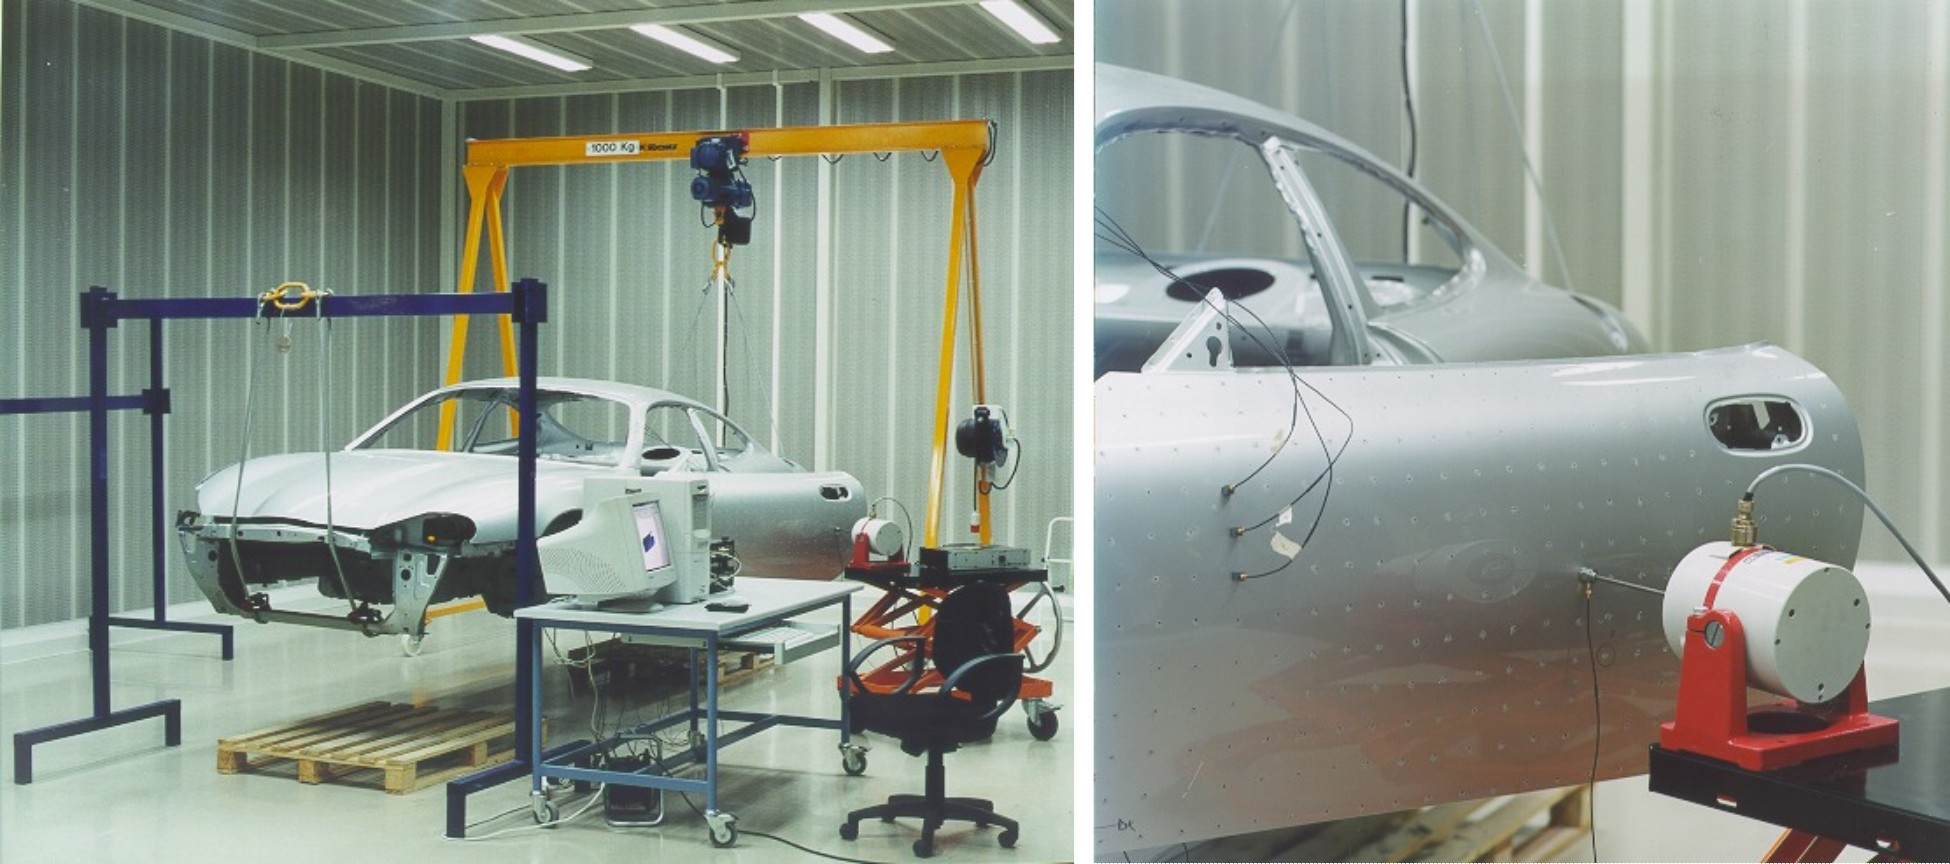
\includegraphics[width=6in]{../figures/modal_testing}
			\caption{Experimental modal analysis of an automotive (Jaguar) body in white, typically done to reduce vehicle noise and vibration harshness \protect\footnotemark[1].}
		\end{figure}
		\footnotetext[1]{Cjp24, CC BY-SA 3.0 $<$https://creativecommons.org/licenses/by-sa/3.0$>$, via Wikimedia Commons} 	
	\end{vibration_case_study}
	
	
	
	 
	
	Mode shapes are not the displacement of a system, rather they describe the configurations into which a structure will naturally displace at a given frequency. For example, consider the 4-DOF system shown in figure~\ref{fig:general_mode_shapes} that represents a pole (i.e. cantilever beam). Assuming that the system experiences a linear response and using the mode-superposition method we can see that the displaced shape $\vec{x}$ is a function of all of the mode shapes $u_i$ and their corresponding participation factors $q_i$. Note that the mode shapes associated with the lower frequencies tend to provide the greatest contribution to structural response. As the frequencies that excite the modes increase, the mode shapes contribute less, are predicted less reliably, and are harder to measure. Therefore, the analysis of the system is often truncated after the first few modes and rarely exceeds the 10$^{\text{th}}$ mode. 
	
	Figure~\ref{fig:general_mode_shapes} shows a structure with $N$ degrees of freedom that therefore had $N$ corresponding mode shapes. Each mode shape is independent and normalized such that the maximum displacements are the same. The summation of the mode shapes multiplied by their corresponding participation factors ($q_i$) yields the deflection of the structure. 
	
	
	\begin{figure}[H]
		\centering
		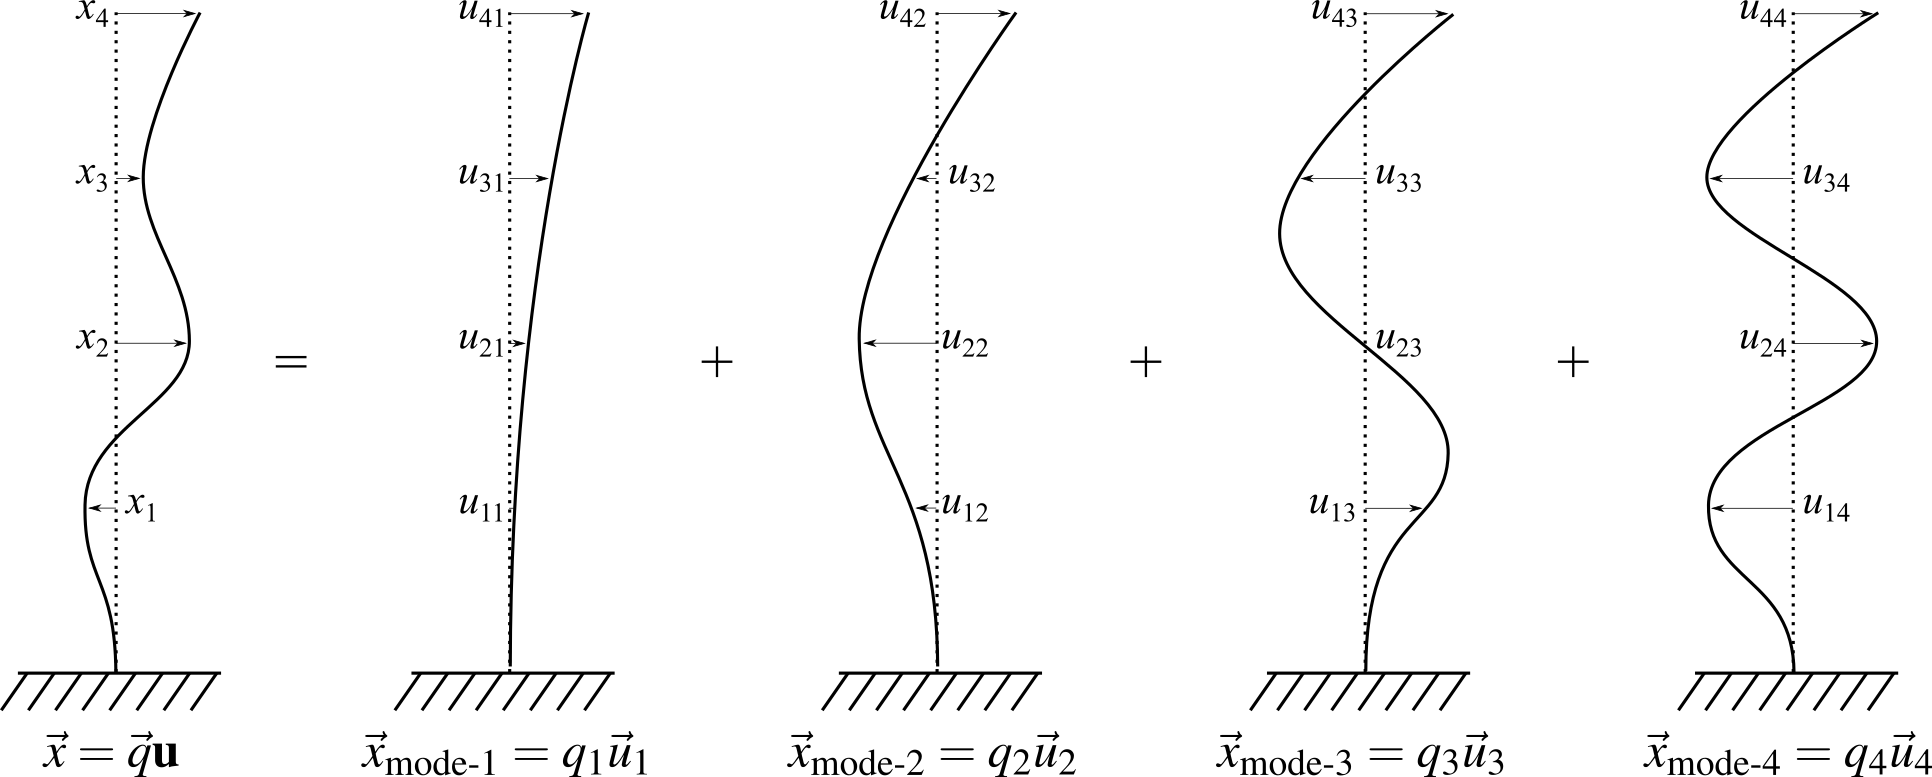
\includegraphics[]{../figures/general_mode_shapes.png}
		\caption{Deflection of a vertical cantilever, $\vec{x}$, is a function of the considered mode shapes $u_i$ and their corresponding participation factors $q_i$.}
		\label{fig:general_mode_shapes}
	\end{figure}
	
	
	
	
	
	\subsection{Modeling Undamped Two Degree of Freedom Systems}
	\label{sec:two_degree_of_freedom}
	
	Consider the undamped 2-DOF systems presented in figure \ref{fig:2-DOF-spring_mass_examples}. This system with a single mass capable of moving in two directions. To expand, figure \ref{fig:2-DOF-spring_mass_examples}(a) reports a mass that can move horizontally or vertically in space. However, this mass does not rotate during its movements. Moreover, figure \ref{fig:2-DOF-spring_mass_examples}(b) presents a system that rotates about the spring and displaces vertically. These are examples of 2 DOF systems because each system has two independent coordinate systems that express the movement of the mass. 
	
	\begin{figure}[H]
		\centering
		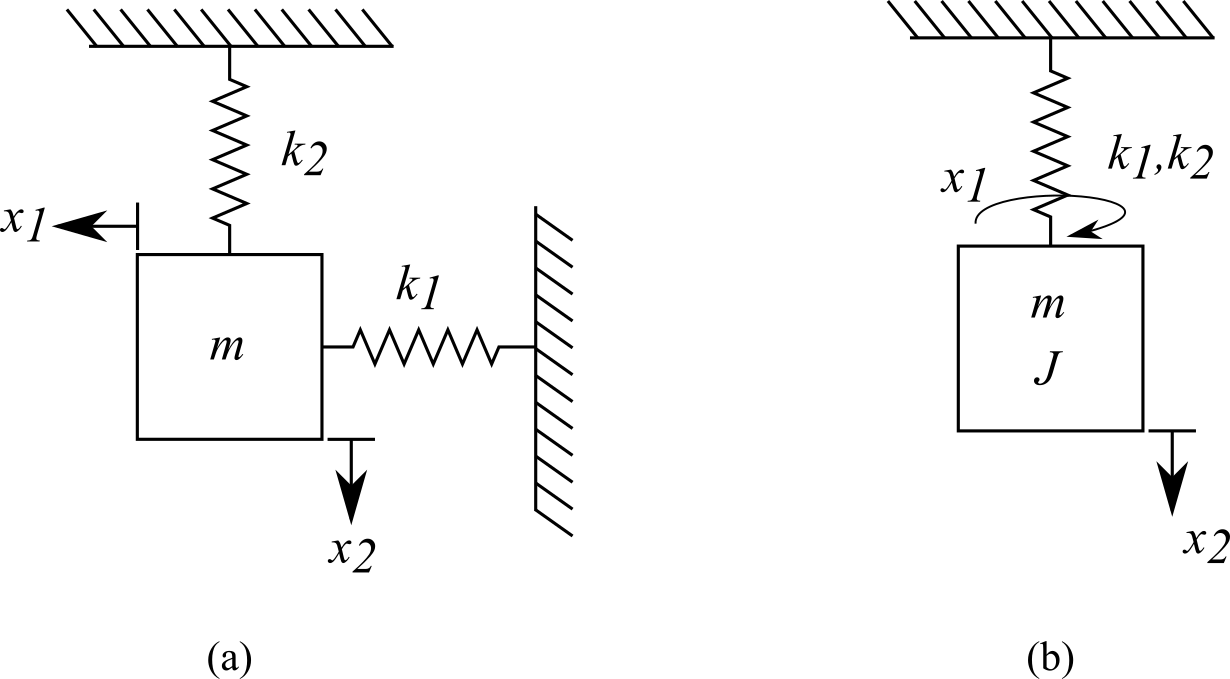
\includegraphics[]{../figures/2-DOF-spring_mass_examples.png}
		\caption{Examples of single mass 2-DOF systems that: (a) displaces in the vertical and horizontal directions, and; (b) rotates about the spring and displaces in the vertical direction. }
		\label{fig:2-DOF-spring_mass_examples}
	\end{figure}
	
	Another example of a 2-DOF system with two masses, each with their own independent coordinate system, is presented in figure \ref{fig:2-DOF-spring_mass_horizontal}. The two coordinates that describe the system's movements are $x_1$ and $x_2$.
	
	\begin{figure}[H]
		\centering
		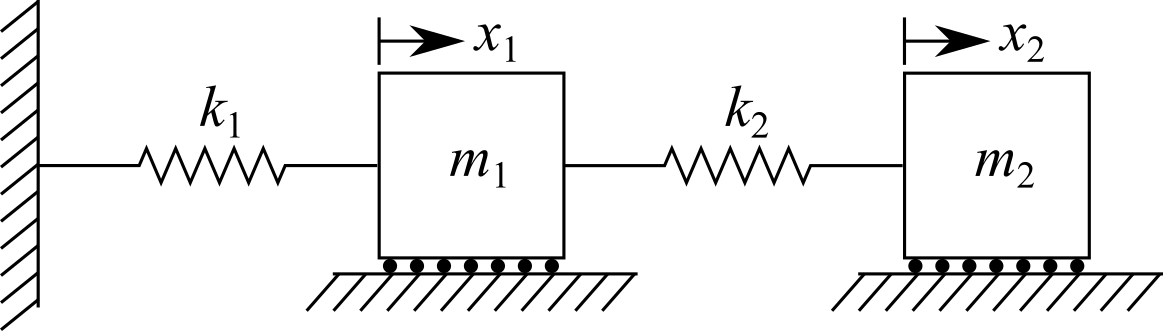
\includegraphics[]{../figures/2-DOF-spring_mass_horizontal.png}
		\caption{2-DOF system with two masses and two independent coordinate systems $x_1$ and $x_2$.}
		\label{fig:2-DOF-spring_mass_horizontal}
	\end{figure}
	
	\subsubsection{Solution for the Two-Degree-of-Freedom System}
	Before we derive a model for undamped 2-DOF systems, let us first consider the solution to the system shown in figure \ref{fig:2-DOF-spring_mass_horizontal}. The solution consists of two equations, one for each mass. This solution will be derived in section \ref{sec:2-DOF_derive_solution} and is expressed by the coupled equations:
	\begin{equation}
		x_1(t) = A_1 \sin (\omega_1 t + \phi_1 )u_{11}+ A_2 \sin (\omega_2 t + \phi_2 )u_{12} \hspace{3.35cm} 
	\end{equation}
	\begin{equation}
		x_2(t) = A_1 \sin (\omega_1 t + \phi_1 )u_{21}+ A_2 \sin (\omega_2 t + \phi_2 )u_{22} , \hspace{1cm} \omega_1 \text{ or } \omega_2 \neq 0 \nonumber
	\end{equation}
	These two equations can be written as a single equation in matrix form as:
	\begin{equation}
		\vec{x}(t) = A_1 \sin (\omega_1 t + \phi_1 )\vec{u}_1 + A_2 \sin (\omega_2 t + \phi_2 )\vec{u}_2 , \hspace{1cm} \omega_1 \text{ or } \omega_2 \neq 0
		\label{eq:2-DOF_solution}
	\end{equation}
	Where the arrow above the variable denotes a vector. Therefore, the vectors $\vec{u}_1$ and $\vec{u}_2$ are the mathematical expressions that ``couple'' or tie the equations together. Expanding these vectors shows: 
	\begin{eqnarray}
	 \vec{x}(t)=  \begin{bmatrix} x_1(t) \\  x_2(t) \end{bmatrix}, \hspace{2ex} \vec{u}_1=  \begin{bmatrix} u_{11} \\  u_{21} \end{bmatrix}, \hspace{2ex} \vec{u}_2=  \begin{bmatrix} u_{12} \\  u_{22} \end{bmatrix}\text{, }
	\end{eqnarray}
	The four key components of the solution expressed in equation \ref{eq:2-DOF_solution} are:
	\begin{enumerate}
	\item $\omega_1$ and $\omega_2$ are the natural frequencies of the system. They are not the frequencies of the masses. The solution states that each of the masses oscillates at the two frequencies $\omega_1$ and $\omega_2$. Moreover, consider the special case where the initial conditions are selected to force $A_2 = 0$, in this case, each mass would only oscillate at only one frequency, $\omega_1$.
	\item $A_1$ and $A_2$ are the constants of integration and determine the amplitude of the system.
	\item $\phi_1$ and $\phi_2$ represent the phase shift of the system
	\item $\vec{u}_1$ and $\vec{u}_2$ are the first and second mode shapes of the system and couple the system together.
	\end{enumerate}
	
	\subsubsection{Deriving the Solution for the Two-Degree-of-Freedom System}
	\label{sec:2-DOF_derive_solution}
	To derive this solution for the system under consideration an FBD for figure \ref{fig:2-DOF-spring_mass_horizontal} can be constructed for the forces acting on each mass. First we have to make the assumption that $x_1 < x_2$, this allows us to say that $m_2$ pulls on $m_1$ and results in:
	\begin{figure}[H]
		\centering
		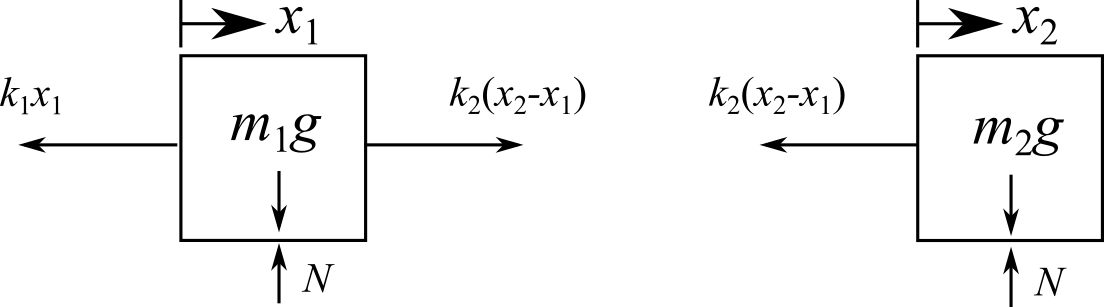
\includegraphics[]{../figures/2-DOF-spring_mass_horizontal_FBD.png}
		\caption{Free body diagram for the 2-DOF system presented in figure \ref{fig:2-DOF-spring_mass_horizontal}.}
		\label{fig:2-DOF-spring_mass_horizontal_FBD}
	\end{figure}
	\noindent Applying Newton's second law and summing the forces on each mass in the horizontal direction yields:
	\begin{eqnarray}
	m_1\ddot{x}_1 &= & -k_1x_1 + k_2(x_2-x_1) \\
	m_2\ddot{x}_2&= & -k_2(x_2-x_1)  \nonumber
	\end{eqnarray}
	These equations can be rearranged in terms of  $x_1$ and $x_2$ as:
	\begin{eqnarray}
	m_1\ddot{x}_1 +(k_1+k_2)x_1 -k_2x_2 =0 \\
	m_2\ddot{x}_2 - k_2x_1 + k_2x_2 = 0 \nonumber
	\end{eqnarray}
	where these are two coupled second-order differential equations that each require two initial conditions to solve. These initial conditions can be obtained from the displacement and velocity terms as:
	\begin{eqnarray}
	x_1(0) = x_{10} \\
	\dot{x}_1(0) = \dot{x}_{10} = v_{10} \nonumber \\ 
	x_2(0) = x_{20} \nonumber \\ 
	\dot{x}_2(0) = \dot{x}_{20} = v_{20} \nonumber
	\end{eqnarray}
	As before, these initial conditions will be the constants of integration used to solve the two second-order differential equations. This solution will provide the free response of each mass in the system. There is a multitude of ways to solve these two coupled second-order differential equations, however, here we will just consider a matrix notation solution. This matrix notation solution is used as this formulation is readably solved using computers and is expandable to more than 2 DOF.
	
	To initiate the solution, let us first develop the matrix formulation of the two coupled ODEs:
	\begin{eqnarray}
	  \begin{bmatrix} m_1 & 0  \\  0 & m_2 \end{bmatrix}\begin{bmatrix} \ddot{x_1} \\  \ddot{x_2} \end{bmatrix} + \begin{bmatrix} k_1+k_2 & -k_2  \\  -k_2 & k_2 \end{bmatrix}\begin{bmatrix} x_1 \\  x_2 \end{bmatrix} = \begin{bmatrix} 0 \\  0 \end{bmatrix}
	\end{eqnarray}
	This equation can also be expressed as the vector equation:
	\begin{equation}
	M\ddot{\vec{x}} + K\vec{x} =0
	\end{equation}
	and is known as the EOM in vector form. In this formulation, the mass matrix ($M$) is defined as:
	\begin{eqnarray}
	 M=  \begin{bmatrix} m_1 & 0  \\  0 & m_2 \end{bmatrix}  
	\end{eqnarray}
	while the stiffness matrix ($K$) is:
	\begin{eqnarray}
	 K=  \begin{bmatrix} k_1+k_2 & -k_2  \\  -k_2 & k_2 \end{bmatrix}
	\end{eqnarray}
	along with the displacement, velocity, and acceleration matrices:
	\begin{eqnarray}
	 \vec{x}=  \begin{bmatrix} x_1 \\  x_2 \end{bmatrix} , \hspace{2ex} \dot{\vec{x}}=  \begin{bmatrix} \dot{x}_1 \\  \dot{x}_2 \end{bmatrix}, \hspace{2ex} \ddot{\vec{x}}=  \begin{bmatrix} \ddot{x}_1 \\  \ddot{x}_2 \end{bmatrix}
	\end{eqnarray}
	Beyond these equations, we can write the initial conditions as:
	\begin{eqnarray}
	\vec{x}_0=  \begin{bmatrix} x_1(0) \\  x_2(0) \end{bmatrix},  \hspace{1cm} \dot{\vec{x}}_0=  \begin{bmatrix} \dot{x}_1(0) \\  \dot{x}_2(0) \end{bmatrix}
	\end{eqnarray}
	This simple connection between vibration analysis and matrix analysis allows computers to be used to solve large and complicated vibration problems quickly.
	
	Recall that the 1-DOF version of the equation of motion was solved by calculating the values of the constants in an assumed harmonic solution. The same approach is applied here in order to solve for the displacement of the two-DOF system. This time, the solution is assumed in the form:
	
	\begin{equation}
		\vec{x}(t) = \vec{u}e^{j\omega t}
	\end{equation}
	where $\vec{u}$ is a vector of constants to be demerited and can be written as:
	\begin{eqnarray}
	\vec{u}=  \begin{bmatrix} u_1 \\  u_2 \end{bmatrix}
	\end{eqnarray}
	From before, $\omega$ is also a constant to be determined. Again, $j=\sqrt{-1}$. In the same manner as before, $e^{j\omega t}$ represents harmonic motion as $e^{j\omega t} = \cos(\omega t) + j \sin(\omega t)$. Taking the derivatives of $\vec{x}(t) = \vec{u}e^{j\omega t}$ yields:
	\begin{equation}
		\dot{\vec{x}}(t) = j\omega\vec{u}e^{j\omega t}
	\end{equation}
	\begin{equation}
		\ddot{\vec{x}}(t) = -\omega^2\vec{u}e^{j\omega t}
	\end{equation}
	Substituting this into the EOM in vector form ($M\ddot{\vec{x}} + K\vec{x} =0$) yields:
	\begin{equation}
	-\omega^2 M  \vec{u}e^{j\omega t} + K\vec{u}e^{j\omega t} =0
	\end{equation}
	or 
	\begin{equation}
	(-\omega^2 M  + K)\vec{u}e^{j\omega t} =0
	\end{equation}
	As $e^{j\omega t} \neq 0$ for any value of $t$ and not allowing $\vec{u}$ to be zero it can be demerited that $(-\omega^2 M  + K)$ must satisfy the vector equation. Therefore,
	\begin{equation}
	(-\omega^2 M  + K)\vec{u} =0, \hspace{1cm} \vec{u}\neq0
	\end{equation}
	This forms a homogeneous set of algebraic equations. To be useful, these equations have a nonzero solution for the system must exist. For this to be true, the inverse of the coefficient matrix $(-\omega^2 M  + K)$ must not exist. To expand, assume that the inverse of $(-\omega^2 M  + K)$ does exist, by multiplying both sides of the equation by $(-\omega^2 M  + K)^{-1}$ yields $\vec{u}=0$. This is a trivial solution (it is not useful) as no motion in the system is implied. Therefore, the logical connection can be drawn between the solution of the equation and the inverse of the coefficient matrix $(-\omega^2 M  + K)$.
	
	Applying the singularity condition to the coefficient matrix of equation $(-\omega^2 M  + K)\vec{u} =0, \hspace{1ex} \vec{u}\neq0$ results a nonzero solution of $\vec{u}$. However, for this to exist the following must be true:
	\begin{equation}
	\det(-\omega^2 M  + K) = 0
	\end{equation}
	Solving this expression results in one algebraic equation with one unknown ($\omega$). Expanding the above equation to consider the values for the matrices $M$ and $K$ results in:
	\begin{eqnarray}
	\det\begin{bmatrix} -\omega^2 m_1 + k_1 + k_2 & -k_2  \\  -k_2 & -\omega^2 m_2 + k_2 \end{bmatrix}=0
	\end{eqnarray}
	Using the definition of the determinant yields that the unknown quantity $\omega^2$ must satisfy:
	\begin{equation}
	m_1 m_2 \omega^4 - (m_1 k_2 + m_2 k_1 + m_2 k_2)\omega^2 + k_1 k_2 = 0
	\label{eq:characteristic_equation}
	\end{equation}
	This expression is called the characteristic equation for the system and is used to determine the constants $\omega_{1,2}$, in the assumed form of the solution given by the assumed solution $\vec{x}(t) = \vec{u}e^{j\omega t}$, once the values of the physical parameters $m_1$, $m_2$, $k_1$, and $k_2$ are known. Note that $\omega_{1,2}$ are not in the characteristic equation, therefore, solving for $\omega_{1,2}$  will be done by factoring the equation above to obtain two solutions $\omega_1$ and $\omega_2$. The characteristic equation is in the form of the quadratic formula if you set $x=\omega^2$, as:
	\begin{equation}
	ax^2 + bx +c = 0
	\end{equation}
	
	After finding the value of $\omega_{1,2}$ using the characteristic equation, the values in $\vec{u}$ can be found using equation $(-\omega^2 M  + K)\vec{u} =0, \hspace{1ex} \vec{u}\neq0$ for each value of $\omega^2$. That is, for both $\omega_1$ and $\omega_2$ there is a vector  $\vec{u}$ that satisfies the equation. These solutions can be written as:
	\begin{equation}
		(-\omega_1^2 M  + K)\vec{u}_1 =0
	\end{equation}
	and 
	\begin{equation}
		(-\omega_2^2 M  + K)\vec{u}_2 =0
	\end{equation}
	The direction of the vectors $\vec{u}_1$ and $\vec{u}_2$ can be obtained by solving the above expressions, however, the information regarding the magnitude of is not contained in this expression. To verify this, assume that $\vec{u}_1$ satisfies the equation, therefore, the vector $a\vec{u}_1$ also satisfies the equation where $a$ is any nonzero number. Hence the vectors satisfying the above are of arbitrary magnitude.
	 
	The values obtained for $\vec{u}_1$ and $\vec{u}_2$ can now be combined with the assumed solution:
	\begin{equation}
		\vec{x}(t) = \vec{u}e^{j\omega t}
	\end{equation}
	to form a set of solutions:
	\begin{equation}
		\vec{x}(t) = \vec{u}_1e^{-j\omega_1 t}, \hspace{2ex} \vec{u}_1e^{j\omega_1 t}, \hspace{2ex} \vec{u}_2e^{-j\omega_2 t}, \hspace{2ex} \vec{u}_2e^{j\omega_2 t}
	\end{equation}
	Since the equation to be solved is linear, the solution is the sum of these solutions. This results in:
	\begin{equation}
		\vec{x}(t) = (a e^{j\omega_1 t} + b e^{-j\omega_1 t})\vec{u}_1 +(c e^{j\omega_2 t} + d e^{-j\omega_2 t})\vec{u}_2
	\end{equation}
	where $a$, $b$, $c$, and $d$ are the arbitrary constants of integration to be determined by the initial conditions. Applying Euler's formulas for the sin functions (where $\omega_1 \text{ or } \omega_2 \neq 0$) reorganizes this equation as:
	\begin{equation}
		\vec{x}(t) = A_1 \sin (\omega_1 t + \phi_1 )\vec{u}_1 + A_2 \sin (\omega_2 t + \phi_2 )\vec{u}_2 , \hspace{1cm} \omega_1 \text{ or } \omega_2 \neq 0
	\end{equation}
	Another way to write this equation is in the form:
	\begin{equation}
		 \begin{bmatrix} x_1(t) \\  x_2(t) \end{bmatrix} =  \begin{bmatrix} \vec{u}_1 & \vec{u}_2 \end{bmatrix}
		 \begin{bmatrix} A_1 \sin (\omega_1 t + \phi_1 )\\ A_2 \sin (\omega_2 t + \phi_2 )\end{bmatrix}, \hspace{1cm} \omega_1 \text{ or } \omega_2 \neq 0
	\end{equation}
	Where the values for $A_1$ and $A_2$ can be obtained by setting applying the boundary conditions and taking the derivatives of the equations as done in the 1-DOF problems. 
	
	The final form of the equation provides physical insight into the solution of the system. It states that each mass in the system oscillates at both of the natural frequencies of the system ($\omega_1$ and $\omega_2$). Furthermore, the importance of the initial conditions can be understood. Assume that initial conditions are chosen that result in $A_2=0$, this cancels out the second natural frequency such that each mass oscillates at only one frequency,  $\omega_1$. Moreover, the positions of the masses can be determined by the values of the vector $\vec{u}_1$ at any given time. For this reason,  $\vec{u}_1$ is termed the first mode shape of the system. Likewise, if the opposite initial conditions are chosen such that  $A_1=0$, then both system coordinates (e.g., masses in the systems we have studied) will oscillate at $\omega_2$ and again, the positions can be obtained from the vector $\vec{u}_2$. Where $\vec{u}_2$ is termed the second mode shape. The interactions between mode shapes and natural frequencies are very important and form the basis of several areas in the field of vibrations.
	
	\begin{example}
	\label{ex:2-DOF}
	\textbf{Calculating Response of a two-DOF system}

	\noindent Considering the following system:
	\begin{figure}[H]
		\centering
		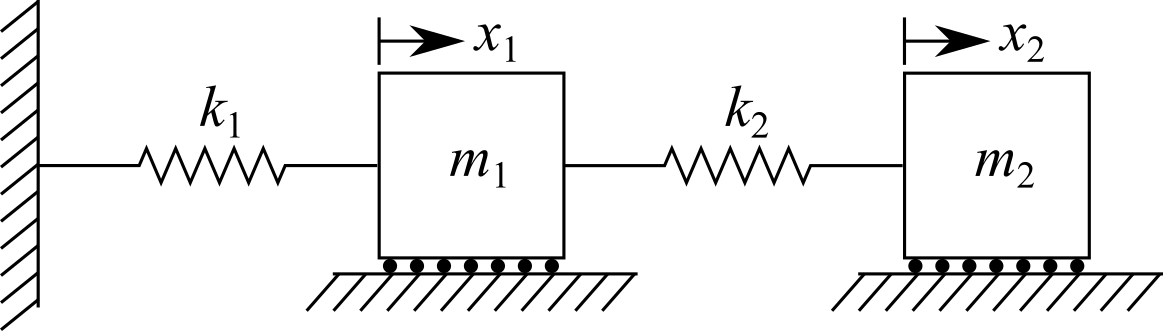
\includegraphics[]{../figures/2-DOF-spring_mass_horizontal.png}
		\caption{2-DOF system with two masses and two independent confidante systems $x_1$ and $x_2$.}
	\end{figure}
	Calculate response for the system if $m_1$=9~kg, $m_2$=1~kg, $k_1$ = 24~N/m, and $k_2$ = 3~N/m with the initial conditions $x_{10}=1$~mm, $v_{10}=0$~mm/s, $x_{20}=0$~mm, and $v_{20}=0$~mm/s. \\
	
	
	\noindent \textbf{Solution:} 

	\noindent  We have already obtained a characteristic equation for this system. This is shown in Equation~\ref{eq:characteristic_equation} and is given as:
	\begin{equation}
	m_1 m_2 \omega^4 - (m_1 k_2 + m_2 k_1 + m_2 k_2)\omega^2 + k_1 k_2 = 0
	\end{equation}
	Substituting our values into this obtains:
	\begin{equation}
	9 \cdot 1 \omega^4 - (9 \cdot 3 + 1 \cdot 24 + 1 \cdot 3)\omega^2 + 24 \cdot 3 = 0
	\end{equation}
	or
	\begin{equation}
	\omega^4 - 6\omega^2 + 8 =0
	\end{equation}
	This can then be factored into:
	\begin{equation}
	(\omega^2-2)(\omega^2-4)=0
	\end{equation}
	This results in solutions of $\omega^2_1 = 2$ and $\omega^2_2 = 4$. Leading to:
	\begin{equation}
	\omega_1 = \pm \sqrt{2} \text{ rad/sec}, \hspace{2ex} \omega_2 = \pm 2 \text{ rad/sec}
	\end{equation}
	
	We need to obtain solutions for $\vec{u}_1$ and $\vec{u}_2$. Having solved for $\omega_1$ and $\omega_2$ we can obtain this. First, knowing $\vec{u}_1 = [u_{11} u_{21}]^\text{T}$ and using $\omega_1 = \sqrt{2}$ and the following equation:
	\begin{equation}
		(-\omega_1^2 M  + K)\vec{u}_1 =0
	\end{equation}
	yields
	simplified to
	\begin{equation}
		 \bigg(-2\begin{bmatrix} 9 & 0 \\   0  & 1 \end{bmatrix} + \begin{bmatrix} 24+3 & -3 \\    -3  & 3 \end{bmatrix}\bigg)\begin{bmatrix} u_{11}\\ u_{21}\end{bmatrix} = \begin{bmatrix} 0\\ 0\end{bmatrix}
	\end{equation}
	simplified to
	\begin{equation}
		 \begin{bmatrix} 27-9\cdot 2 & -3 \\    -3  & 3-2 \end{bmatrix} 
		 \begin{bmatrix} u_{11}\\ u_{21}\end{bmatrix}=\begin{bmatrix} 0\\ 0\end{bmatrix}
	\end{equation}
	or
	\begin{equation}
		 \begin{bmatrix} 9 & -3 \\    -3  & 1 \end{bmatrix} 
		 \begin{bmatrix} u_{11}\\ u_{21}\end{bmatrix}=\begin{bmatrix} 0\\ 0\end{bmatrix}
	\end{equation}
	Taking the dot product of the matrix equation yields:
	\begin{equation}
		9u_{11} -3u_{21}=0 \text{, and } -3u_{12} + u_{22}=0
	\end{equation}
	Both of these equations yield the same equation, that is:
	\begin{equation}
		\frac{u_{11}}{u_{21}} =\frac{1}{3}
	\end{equation}
	As mentioned before, only the ratio of the elements is determined here. To show this is true it is easily seen that:
	\begin{equation}
		u_{11}=u_{21}\frac{1}{3} \rightarrow  a u_{11}= a u_{21}\frac{1}{3} 
	\end{equation}
	To obtain a numerical value, we arbitrarily assign a value to one of the elements. Here, let $u_{21}=1$ so  let $u_{11}=1/3$. Therefore, 
	\begin{equation}
		 \vec{u}_1 = \begin{bmatrix} \frac{1}{3}\\ 1\end{bmatrix}
	\end{equation}
	The same processes can be used for obtaining $\vec{u}_2$ using $\omega_2=2$, this results in:
	\begin{equation}
		 \begin{bmatrix} -9 & -3 \\    -3  & -1 \end{bmatrix} 
		 \begin{bmatrix} u_{12}\\ u_{22}\end{bmatrix}=\begin{bmatrix} 0\\ 0\end{bmatrix}
	\end{equation}
	Taking the dot product of the matrix equation yields:
	\begin{equation}
		-9u_{12} -3u_{22}=0 \text{, and } -3u_{12} - u_{22}=0
	\end{equation}
	Both of these equations yield the same equation, that is:
	\begin{equation}
		\frac{u_{12}}{u_{22}} =-\frac{1}{3}
	\end{equation}
	Again, assuming $u_{22}=1$  this can be rearranged into $\vec{u}_2$ as:
	\begin{equation}
		 \vec{u}_2 = \begin{bmatrix} -\frac{1}{3}\\ 1\end{bmatrix}
	\end{equation}
	Where $\vec{u}_1$ and $\vec{u}_2$ represent only the directions and shape of the mode shapes and not the magnitude of the mode shapes. 

	Now that we have the mode shapes, we can solve for the initial conditions $A_1$ and $A_2$. To do this, let us use the following formulation of the solution:
	\begin{equation}
		 \begin{bmatrix} x_1(t) \\  x_2(t) \end{bmatrix} =  \begin{bmatrix} \vec{u}_1 & \vec{u}_2 \end{bmatrix}
		 \begin{bmatrix} A_1 \sin (\omega_1 t + \phi_1 )\\ A_2 \sin (\omega_2 t + \phi_2 )\end{bmatrix}, \hspace{1cm} \omega_1 \text{ or } \omega_2 \neq 0
	\end{equation}
	Adding our values for the problem at $t=0$ this becomes:
	\begin{equation}
		 \begin{bmatrix} 1 \\  0 \end{bmatrix} =  \begin{bmatrix} \frac{1}{3} & -\frac{1}{3} \\ 1 & 1 \end{bmatrix}
		 \begin{bmatrix} A_1 \sin (\phi_1)\\ A_2 \sin (\phi_2)\end{bmatrix}
	\end{equation}
	and after applying the dot product:
	\begin{equation}
		 \begin{bmatrix} 1 \\  0 \end{bmatrix} =  \begin{bmatrix} \frac{1}{3}A_1 \sin (\phi_1 ) -\frac{1}{3}A_2 \sin (\phi_2)\\ A_1 \sin (\phi_1 )+A_2 \sin (\phi_2 )\end{bmatrix}
	\end{equation}
	Next we can differentiate the equation for $x(t)$ to obtain the velocity solution. Adding our values for the problem at $t=0$ obtains:
	\begin{equation}
		 \begin{bmatrix} \dot{x}_1(0) \\  \dot{x}_2(0) \end{bmatrix}  = \begin{bmatrix} v_{10} \\  v_{20} \end{bmatrix} = \begin{bmatrix} 0 \\  0 \end{bmatrix} =   \begin{bmatrix} \frac{\sqrt{2}}{3}A_1 \cos (\phi_1 ) -\frac{2}{3}A_2 \cos (\phi_2)\\ \sqrt{2}A_1 \cos (\phi_1 )+2 A_2 \cos (\phi_2 )\end{bmatrix}
	\end{equation}
	Now that we have 4 equations for 4 unknowns we can use these equations to solve for $A_1$,  $A_2$, $\phi_1$,  and $\phi_2$. The 4 equations are:
	\begin{equation}
	3= A_1 \sin (\phi_1 ) - A_2 \sin (\phi_2)
	\end{equation}
	\begin{equation}
	0= A_1 \sin (\phi_1 ) + A_2 \sin (\phi_2)
	\end{equation}
	\begin{equation}
	0= \sqrt{2}A_1 \cos (\phi_1 ) - 2A_2 \cos (\phi_2)
	\end{equation}
	\begin{equation}
	0= \sqrt{2}A_1 \cos (\phi_1 ) + 2A_2 \cos (\phi_2)
	\end{equation}
	Setting these last two equations equal to each other yields:
	\begin{equation}
	0= \sqrt{2}A_1 \cos (\phi_1 ) + 2A_2 \cos (\phi_2) = \sqrt{2}A_1 \cos (\phi_1 ) - 2A_2 \cos (\phi_2)
	\end{equation}
	or:
	\begin{equation}
	0= - 4A_2 \cos (\phi_2)
	\end{equation}
	For this equation to be true, $\phi_2=\frac{\pi}{2}$. Therefore, applying this to $0= \sqrt{2}A_1 \cos (\phi_1 ) + 2A_2 \cos (\phi_2)$ results in:
	\begin{equation}
	0= \sqrt{2}A_1 \cos (\phi_1 )
	\end{equation}
	where again, for this equation to be true, $\phi_1=\frac{\pi}{2}$. Now the first two equations become:
	\begin{equation}
	3= A_1 - A_2 
	\end{equation}
	\begin{equation}
	0= A_1 + A_2 
	\end{equation}
	Where this shows us that $A_1 = \frac{3}{2}$ and $A_2 = -\frac{3}{2}$. 

	Now that we have the initial conditions we can find a solution for the temporal response of each mass. Using the equations from before:
	\begin{equation}
		x_1(t) = A_1 \sin (\omega_1 t + \phi_1 )u_{11} + A_2 \sin (\omega_2 t + \phi_2 )u_{12}
	\end{equation}
	\begin{equation}
		x_2(t) = A_1 \sin (\omega_1 t + \phi_1 )u_{21} + A_2 \sin (\omega_2 t + \phi_2 )u_{22}
	\end{equation}
	And applying our obtained values
	\begin{equation}
		x_1(t) = \frac{3}{2} \sin (\sqrt{2} t + \frac{\pi}{2} )\frac{1}{3} + \bigg(-\frac{3}{2}\bigg) \sin (2 t + \frac{\pi}{2} ) \bigg(-\frac{1}{3}\bigg)
	\end{equation}
	\begin{equation}
		x_2(t) = \frac{3}{2} \sin (\sqrt{2} t + \frac{\pi}{2} ) + \bigg(-\frac{3}{2}\bigg) \sin (2 t + \frac{\pi}{2} )
	\end{equation}
	results in:
	\begin{equation}
		x_1(t) = \frac{1}{2} \bigg(  \sin (\sqrt{2} t + \frac{\pi}{2} ) + \sin (2 t + \frac{\pi}{2} ) \bigg)
	\end{equation}
	\begin{equation}
		x_2(t) = \frac{3}{2}  \bigg( \sin (\sqrt{2} t + \frac{\pi}{2} ) -\sin (2 t + \frac{\pi}{2} ) \bigg)
	\end{equation}
	These results can be plotted as:
	\begin{figure}[H]
		\centering
		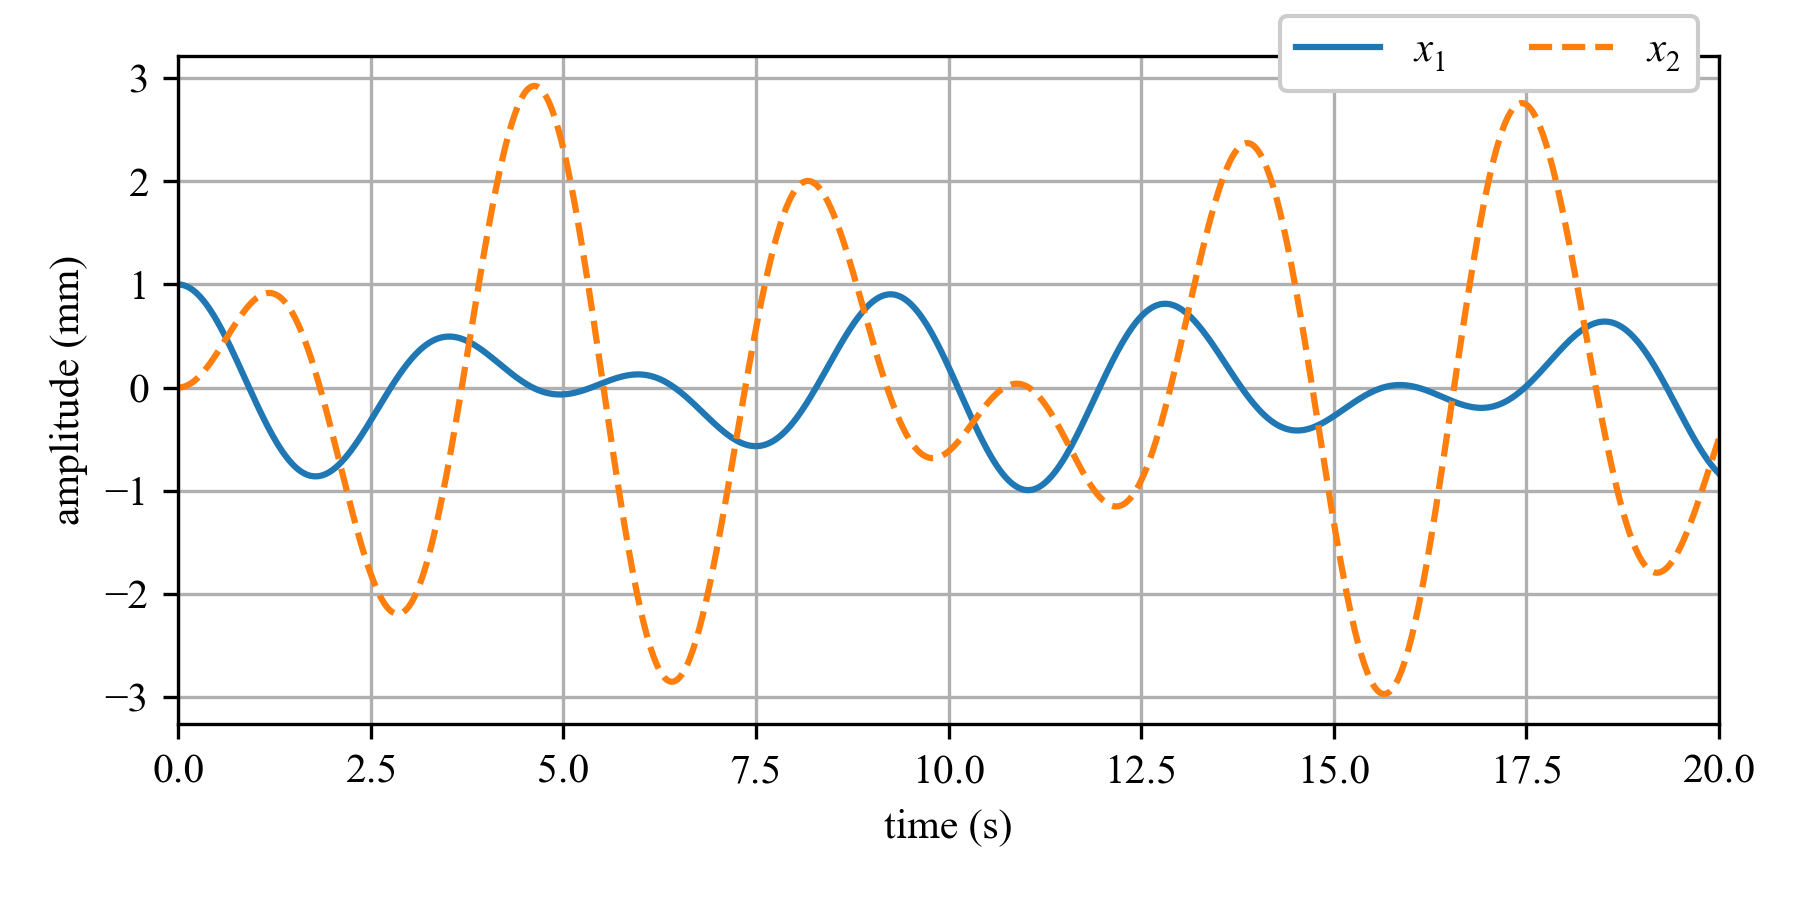
\includegraphics[width=0.9\textwidth]{../figures/2-DOF_response.png}
		\caption{Temporal response for each of the rigid bodies in the 2-DOF system.}
	\end{figure}
	\end{example}
	
	
	
	
	
	\begin{example}

	\textbf{Plotting Mode Shapes}

	\noindent Mode shapes can be better understood through a graphical representation. To do this, consider the 2-DOF system presented in figure \ref{fig:2-DOF-spring_mass_vertical}(a). Assuming that $x_1<x_2$ the FBD for the system is expressed in figure \ref{fig:2-DOF-spring_mass_vertical}(b).
	
	\begin{figure}[H]
		\centering
		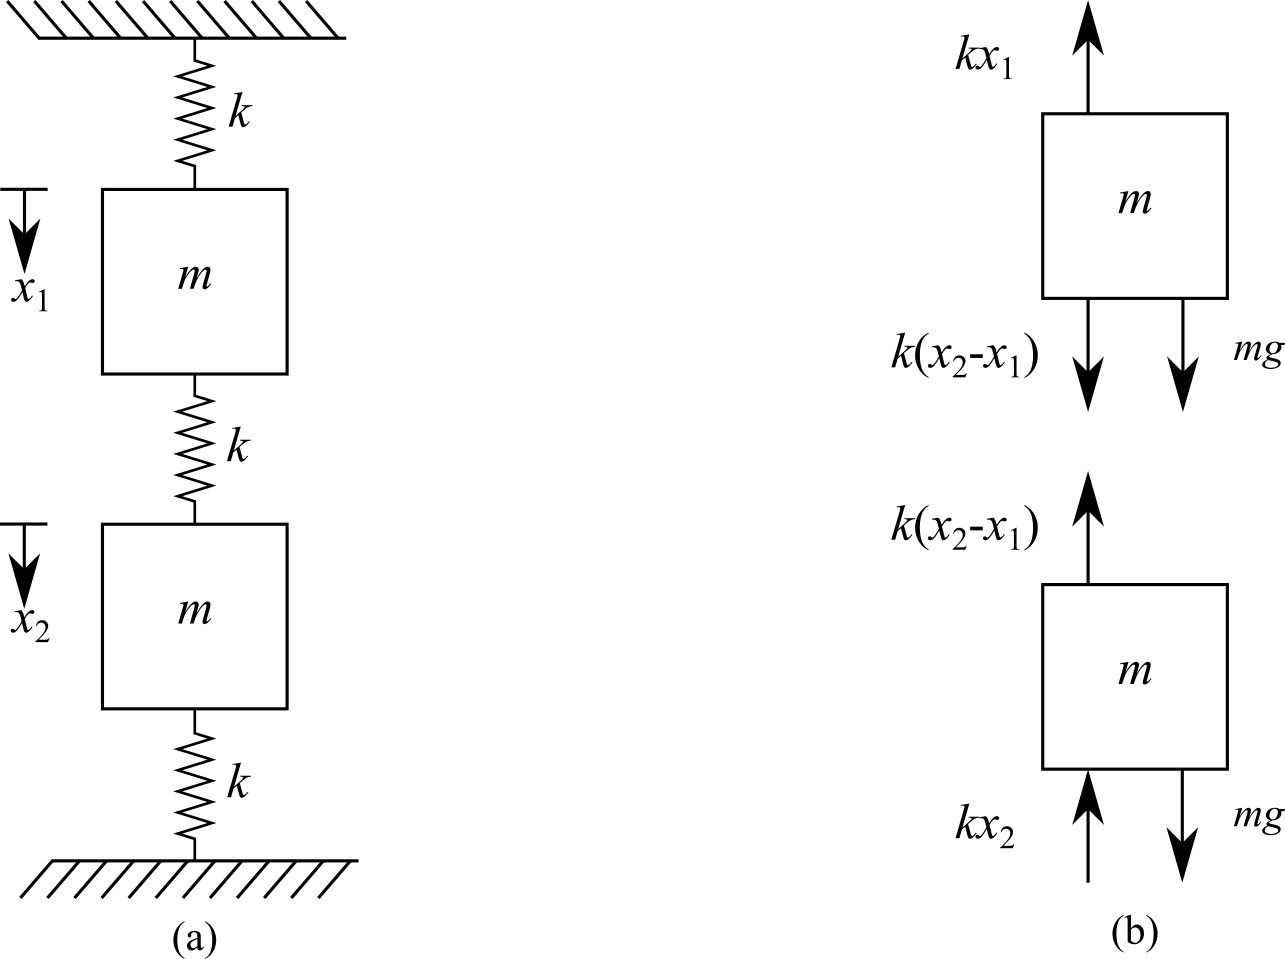
\includegraphics[]{../figures/2-DOF-spring_mass_vertical_with_FBD.png}
		\caption{(a) 2-DOF system with two masses arranged in a vertical configuration; and (b) FBD of system.}
		\label{fig:2-DOF-spring_mass_vertical}
	\end{figure}
	\noindent For simplicity, all masses, and spring stiffness are considered equal and that $m=1$ and $k=1$. \\

	\noindent \textbf{Solution:} 

	\noindent  From the previous investigations in this text, we know that the forces caused by gravity will cancel out. Therefore, the EOM for the system can be written as:
	\begin{eqnarray}
	m\ddot{x}_1 &= & -kx_1 + k(x_2-x_1) \\
	m\ddot{x}_2&= & -k(x_2-x_1) -kx_2 \nonumber
	\end{eqnarray}
	These equations can be written in matrix notation as:
	\begin{eqnarray}
		\begin{bmatrix} m & 0  \\  0 & m \end{bmatrix}\begin{bmatrix} \ddot{x_1} \\  \ddot{x_2} \end{bmatrix} + \begin{bmatrix} 2k & -k  \\  -k & 2k \end{bmatrix}\begin{bmatrix} x_1 \\  x_2 \end{bmatrix} = \begin{bmatrix} 0 \\  0 \end{bmatrix}
	\end{eqnarray}
	Substituting the values of the matrices $M$ and $K$ into this expression $\det(-\omega^2 M  + K) = 0$ yields: 
	\begin{eqnarray}
	\det\begin{bmatrix} -\omega^2 m + 2k & -k  \\  -k & -\omega^2 m + 2k \end{bmatrix}=0
	\end{eqnarray}
	The determinant yields that the unknown quantity, $\omega^2$, must satisfy:
	\begin{equation}
	m^2 \omega^4 - 4km\omega^2 + 3k^2 = 0
	\end{equation}
	using the quadratic formula we obtain
	\begin{equation}
	\omega_1 = \pm \sqrt{\frac{k}{m}}=1 \text{ rad/sec}, \hspace{2ex} \omega_2 = \pm \sqrt{\frac{3k}{m}}=\sqrt{3} \text{ rad/sec}
	\end{equation}
	Now, we need to obtain solutions for $\vec{u}_1$ and $\vec{u}_2$. Knowing $(-\omega_1^2 M  + K)\vec{u}_1 =0$ yields:
	\begin{equation}
		 \begin{bmatrix} 1 & -1 \\    -1  & 1 \end{bmatrix} 
		 \begin{bmatrix} u_{11}\\ u_{21}\end{bmatrix}=\begin{bmatrix} 0\\ 0\end{bmatrix}
	\end{equation}
	Taking the dot product of the matrix equation yields:
	\begin{equation}
		u_{11} - u_{21}=0 \text{, and } - u_{12} + u_{22}=0
	\end{equation}
	Setting $u_{11} = 1$ results in $u_{21} = 1$ . The same processes can be performed for $\vec{u}_2$ to show that if we set $u_{12} = 1$, $u_{22} = -1$. Therefore, the mode shapes can be expressed as:
	\begin{equation}
		 \vec{u}_1 = \begin{bmatrix} u_{11} \\ u_{21} \end{bmatrix} = \begin{bmatrix} 1 \\ 1 \end{bmatrix}\text{ and } \vec{u}_2 = \begin{bmatrix} u_{12} \\ u_{22} \end{bmatrix}  = \begin{bmatrix} 1 \\ -1 \end{bmatrix} 
	\end{equation}
	The displacement of the masses as a function of time and the general mode shape plots are graphically represented in figure \ref{fig:2-DOF_mode_shape}. In the 2-DOF system considered here, the second mode shape has a spot at the center of the middle spring that does not move (i.e. has zero displacement). This point is called a node. Nodes correspond to points in the mode shape where the displacement is always zero. Furthermore, the displacement of the node points remain zero at all times, as diagrammed in the top-right of figure \ref{fig:2-DOF_mode_shape}.
	
	\begin{figure}[H]
		\centering
		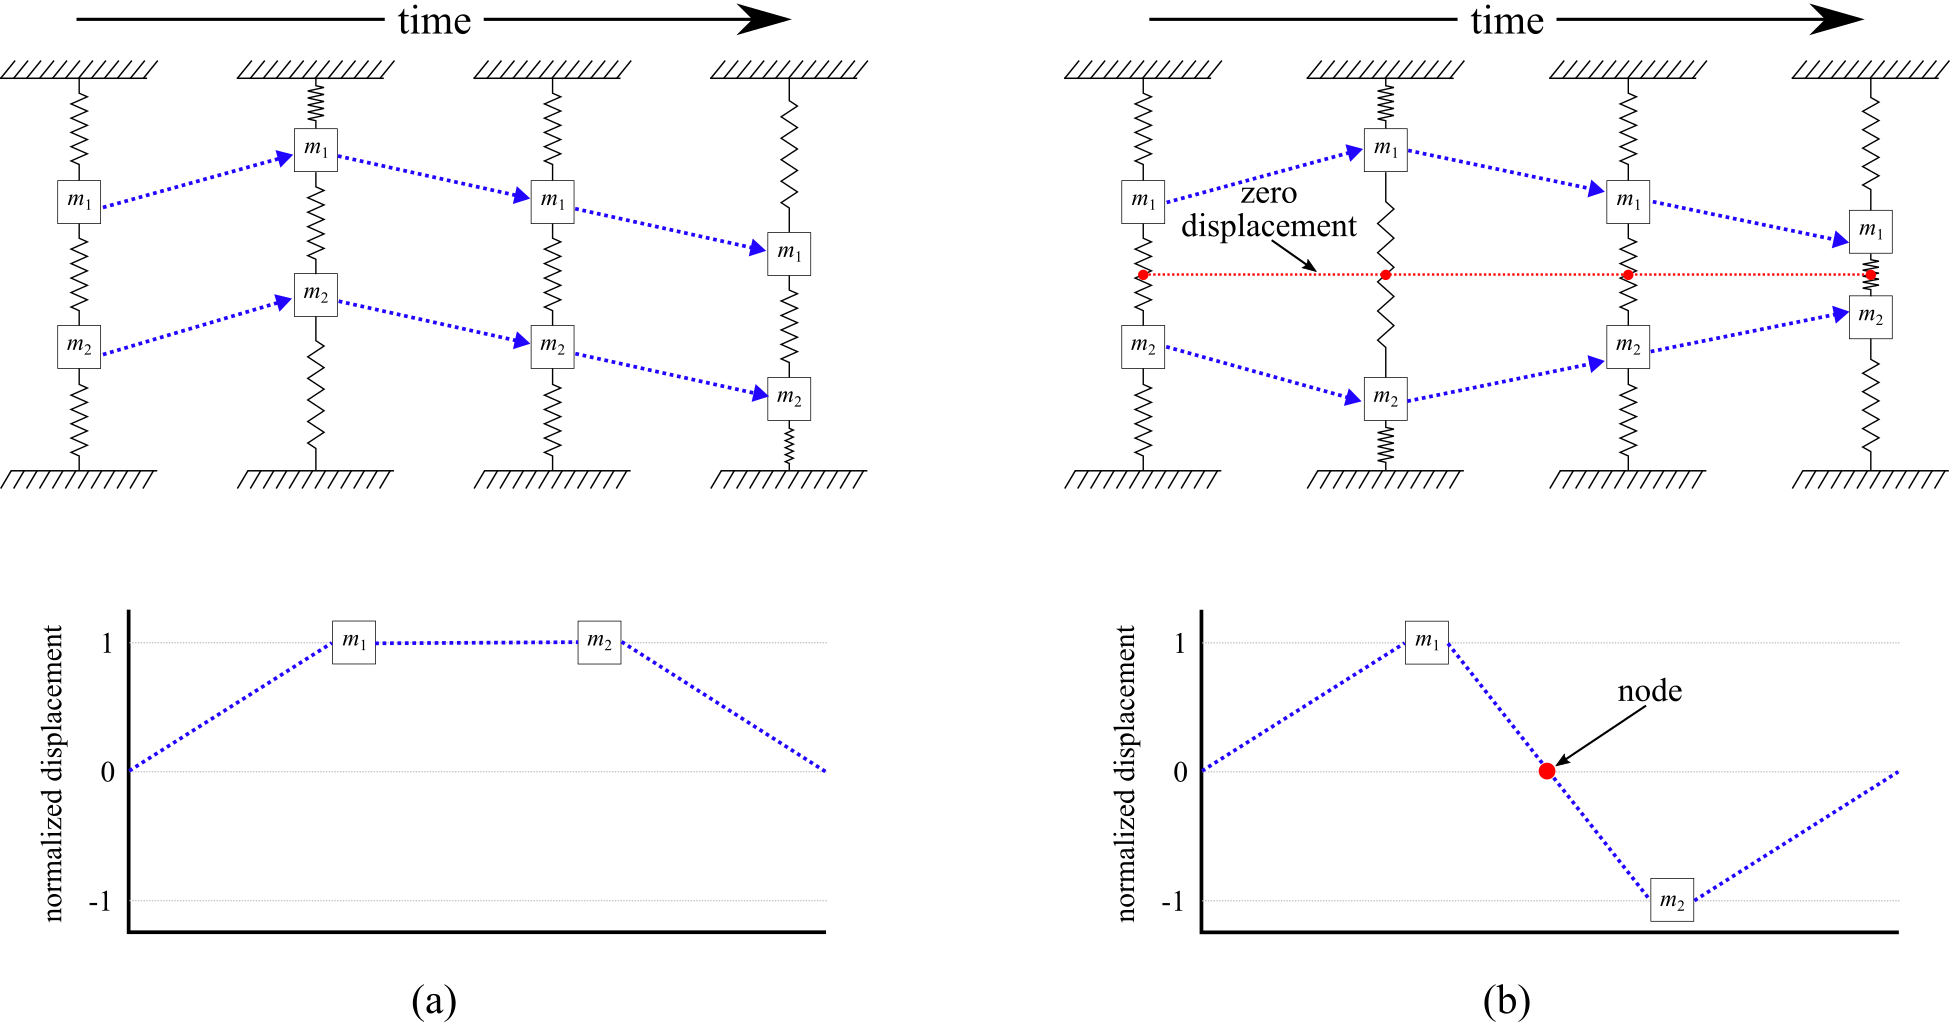
\includegraphics[width=\linewidth]{../figures/2-DOF_mode_shape.png}
		\caption{Modes of vibration for the system shown in figure \ref{fig:2-DOF-spring_mass_vertical} showing the: (a) first mode; and (b) second mode.}
		\label{fig:2-DOF_mode_shape}
	\end{figure}
	\end{example}
	
	
	
	\subsection{Explicit method for Solving 2-DOF Systems}
	
	
	\begin{figure}[H]
		\centering
		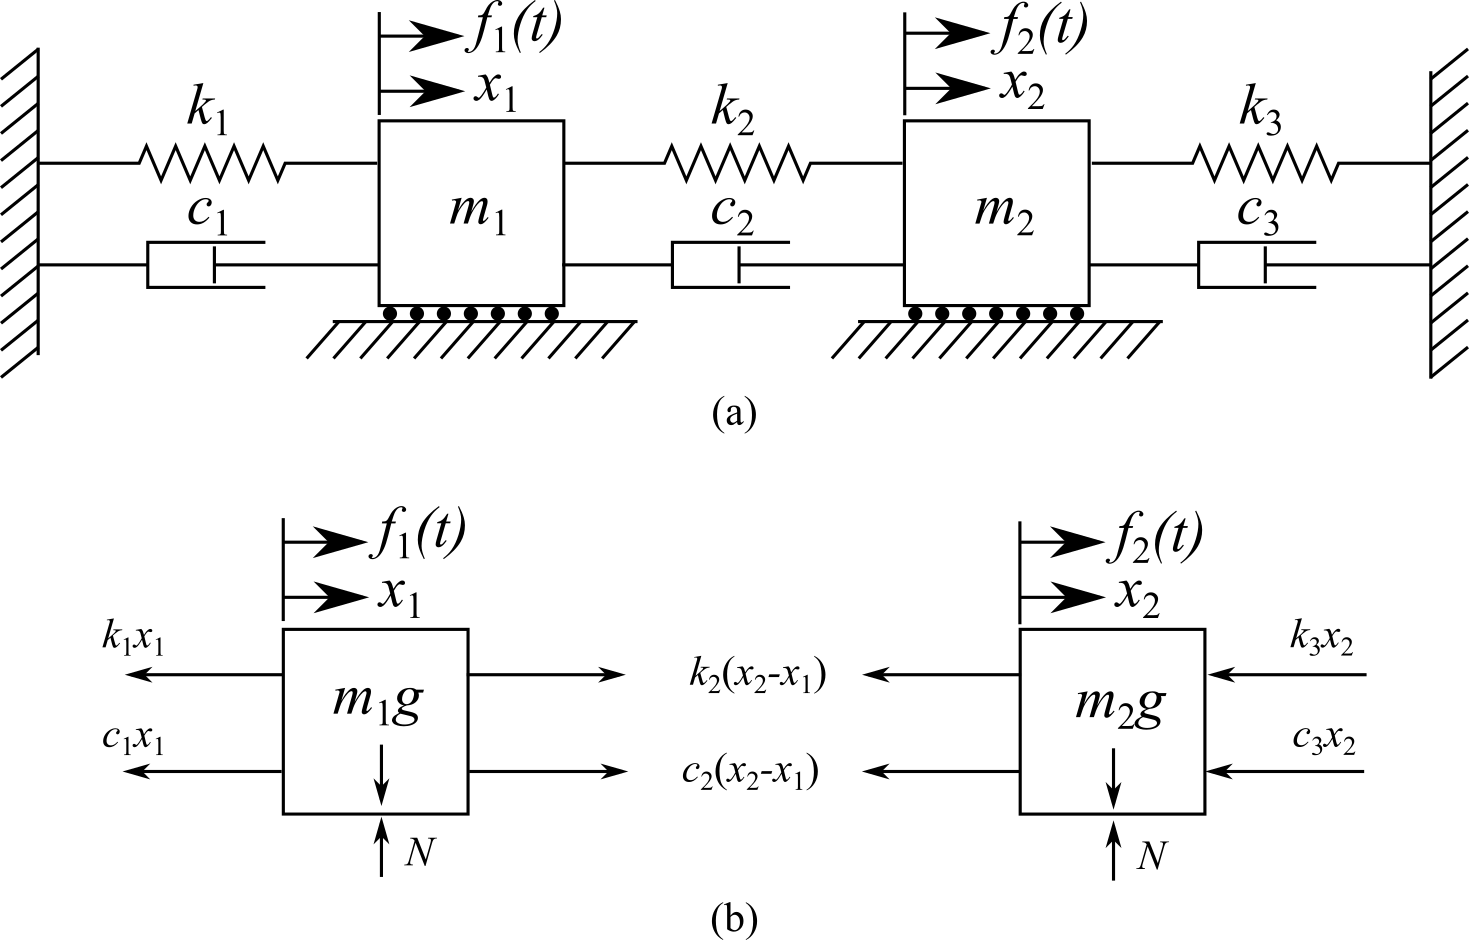
\includegraphics[]{../figures/2-DOF-spring_mass_dashpot_horizontal_forced_double_wall.png}
		\caption{Forced 2-DOF damped system showing: (a) system, and; (b) FBD.}
		\label{fig:2-DOF-spring_mass_dashpot_horizontal_double_wall}
	\end{figure}
	
	
	As before, we can use explicit methods for solving multiple degree of freedom problems. 
	Cramer's rule is an explicit formula for the solution of a system of linear equations with as many equations as unknowns. Cramer's rule is valid whenever the system has a unique solution and can be used as a more generalized approach to solving for the temporal solution to a 2-DOF. Consider the 2-DOF systems shown in figure~\ref{fig:2-DOF-spring_mass_dashpot_horizontal_double_wall}, where $x_2$ displaces more than $x_1$. The two coupled equations of motion are expressed as: 
	\begin{eqnarray}
	m_1\ddot{x}_1 + (c_1+c_2)\dot{x}_1 - c_2\dot{x}_2 + (k_1+k_2)x_1 - k_2x_2 =0 \\
	m_2\ddot{x}_2 + (c_2+c_3)\dot{x}_2 - c_2\dot{x}_1 + (k_2+k_3)x_2 - k_2x_1 =0 \nonumber
	\end{eqnarray}
	As before, taking the Laplace of the EOM (while ignoring the initial conditions) changes the equation from the temporal domain to the complex $s$-plane. This yields:
	\begin{eqnarray}
	m_1 s^2 X_1(s) + (c_1 + c_2)sX_1(s) - c_2sX_2(s) + (k_1+k_2)X_1(s) - k_2X_2(s) = F_1(s) \\
	m_2 s^2 X_2(s) + (c_2 + c_3)sX_2(s) - c_2sX_1(s) + (k_2+k_3)X_2(s) - k_2X_1(s) = F_2(s) \nonumber
	\end{eqnarray}
	these equations can be rearranged in terms of $X_1$ and $X_2$ as follows:
	\begin{equation}
	[m_1 s^2 + (c_1 + c_2)s + (k_1+k_2)]X_1(s) - [c_2s+k_2]X_2(s) = F_1(s) 
	\end{equation}
	\begin{equation}
	[m_2 s^2 + (c_2 + c_3)s + (k_2+k_3)]X_2(s) - [c_2s+k_2]X_1(s) = F_2(s) \nonumber
	\end{equation}
	These equations show two linear equations in terms of $X_1$ and $X_2$ that can be solved for using Cramer's rule, resulting in the expression:
	\begin{eqnarray}
	X_1(s) = \frac{D_1(s)}{D(s)} \\
	X_2(s) = \frac{D_2(s)}{D(s)} \nonumber
	\end{eqnarray}
	where:
	\begin{eqnarray}
	D_1 = \left|
	\begin{array}{cc}
	F_1(s)  & -(c_2s+k_2) \\
	F_2(s)  & m_2 s^2 + (c_2 + c_3)s + (k_2+k_3) \\
	\end{array}
	\right| \\
	= [m_2 s^2 X_2(s) + (c_2 + c_3)s +(k_2+k_3)]F_1(s) + (c_2s+k_2)F_2(s)  \nonumber
	\end{eqnarray}
	
	\begin{eqnarray}
	D_2 = \left|
	\begin{array}{cc}
	m_1 s^2 + (c_1 + c_2)s + (k_1+k_2)  & F_1(s) \\
	-(c_2s+k_2)  & F_2(s) \\
	\end{array}
	\right| \\
	= [m_1 s^2 + (c_1 + c_2)s + (k_1+k_2)]F_2(s) + (c_2s+k_2)F_1(s)  \nonumber
	\end{eqnarray}
	
	\begin{eqnarray}
	D = \left|
	\begin{array}{cc}
	m_1 s^2 + (c_1 + c_2)s + (k_1+k_2) & m_2 s^2 + (c_2 + c_3)s + (k_2+k_3) \\
	-(c_2s+k_2) & -(c_2s+k_2) \\
	\end{array}
	\right| \\ \nonumber
	= m_1m_2s^4 + [m_2(c_1+c_3)+m_1(c_2+c_3)]s^3 \\  \nonumber
	+ [m_2(k_1+k_2)+m_1(k_2+k_3)+c_1c_2+c_2c_3+c_3c_1]s^2 \\  \nonumber
	+ [(k_1+k_2)(c_2+c_3)+c_1k_2+c_1k_3-c_2k_2+c_2k_3]s \\  \nonumber
	+ (k_1k_2 + k_2k_3 + k_3k_1) \\  \nonumber
	\end{eqnarray}
	
	The denominator, $D(s)$ is a 4$^{\text{th}}$ polynomial in $s$ and is the characteristic polynomial of the system. The system is considered a 4$^{\text{th}}$ order system because the characteristic polynomial of the system is of order 4. 
	
	%\begin{example}
	%content...
	%content...
	%content...
	%
	%\rd{Add an example}
	%% \rd{example 5.11 in Rao ed 6 has a good example of this nature.}
	%\end{example}

	
	
	\begin{vibration_case_study}

	\textbf{Closely Coupled Modes in Complex Structures}

	\noindent Multi-span concrete bridges like the Trigno V bridge (figure~\ref{fig:case_study_closely_coupled_bridge_frequencies_1}) over the Trigno river in Italy have repeating segments that make up the bridge decks. The structural components of the segmented bridge decks are separate components sitting on bearing pads and piers where the only connecting material between decks is the overlay that is added to provide a contentious road surface. This configuration forms what is known as a partially-connected bridge deck\protect\footnotemark[1].
	\begin{figure}[H]
		\centering
		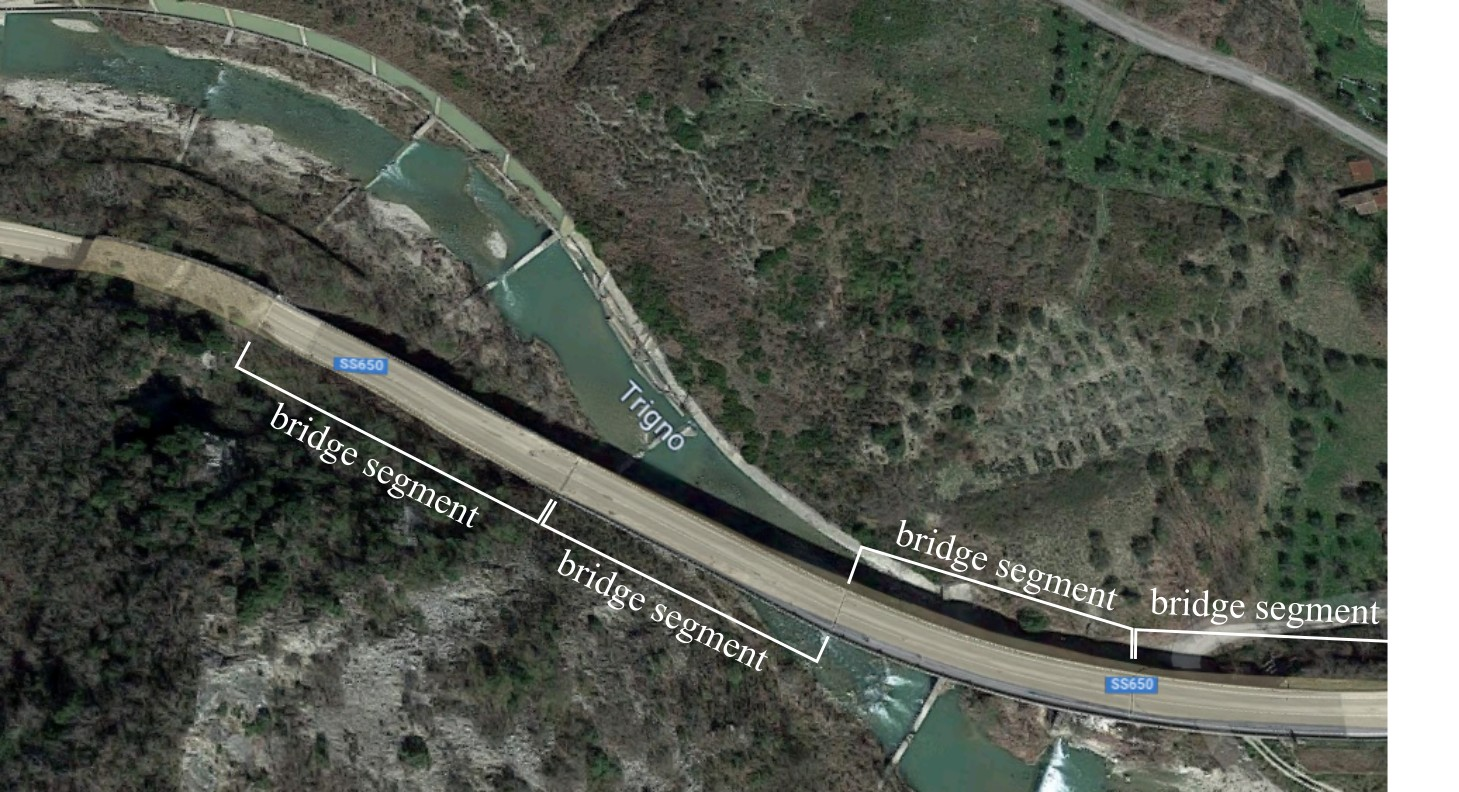
\includegraphics[width=\linewidth]{../figures/case_study_closely_coupled_bridge_frequencies_1}
		\caption{The Trigno V bridge over the Trigno river that carries SS650 north of Trivento Italy is made up of seven repeating concrete bridge deck\protect\footnotemark[2]. }%\footnotetext[1]{Elisa Tomassini, CC BY-SA 4.0 $<$https://creativecommons.org/licenses/by-sa/4.0$>$}.}
		\label{fig:case_study_closely_coupled_bridge_frequencies_1}
		% 41°47'26.0"N 14°32'15.5"E
	\end{figure}
	
	This system can be modeled as a multi-degree of freedom problem. However, the challenge is that with so many nearly identical bridge components, the natural frequencies of each bridge deck will be close, but not identical. This results in a clustering of natural frequencies as shown in figure~\ref{fig:case_study_closely_coupled_bridge_frequencies_2} where the frequencies of the 1\textsuperscript{st} and 2\textsuperscript{nd} modes of the various bridge deck components are clustered in groups and therefore hard to distinguish. Moreover, obtaining the characteristic structural dynamics of any particular bridge deck section would be difficult as the decks are coupled through the pavement overlay making it challenging to isolate the dynamic measurements of just one bridge section. 
	
	\begin{figure}[H]
		\centering
		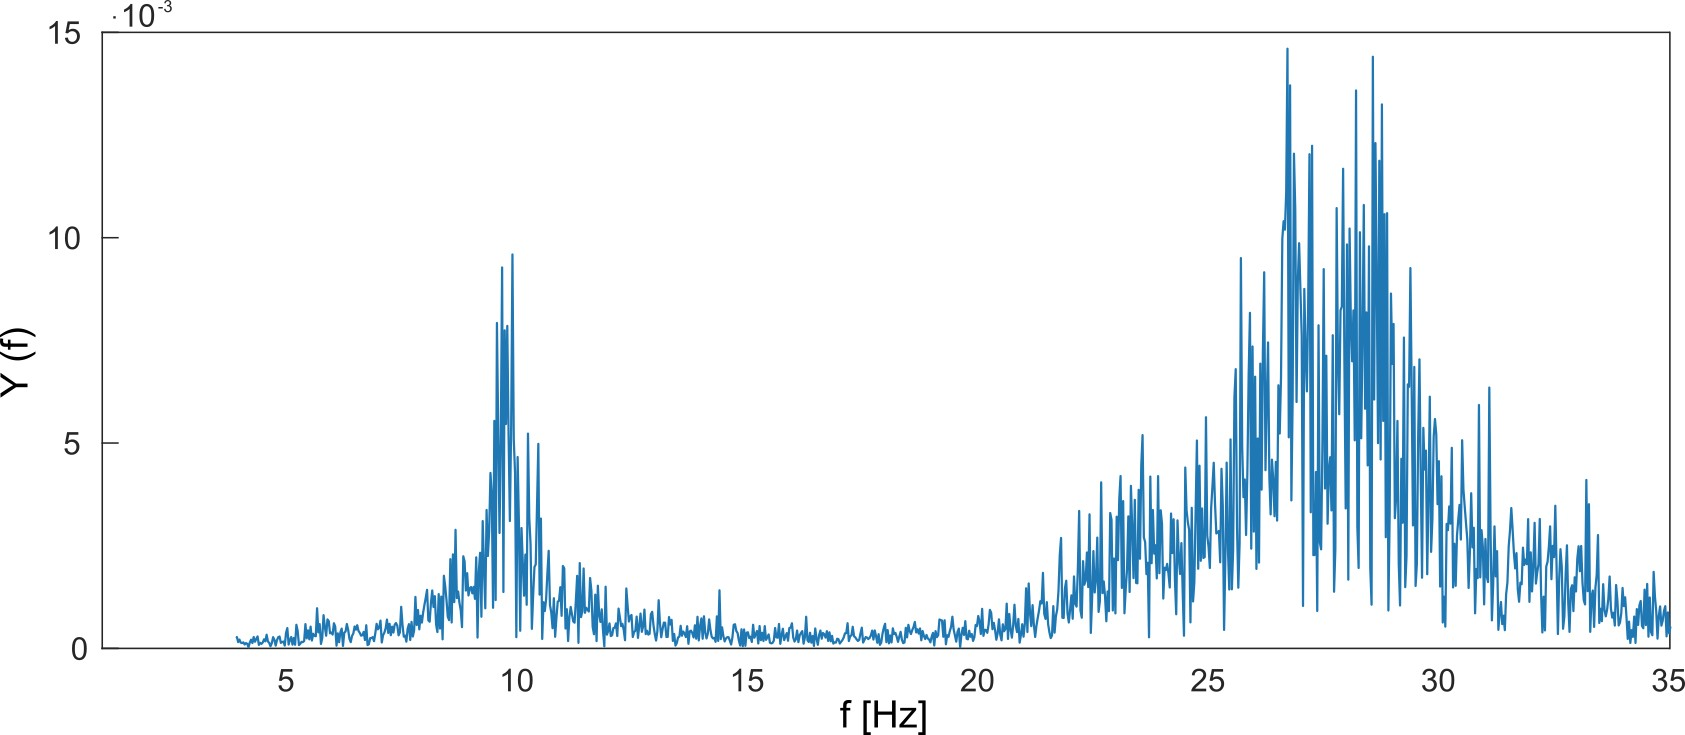
\includegraphics[width=\linewidth]{../figures/case_study_closely_coupled_bridge_frequencies_2}
		\caption{Measured acceleration signal for the bridge showing the estimated 1\textsuperscript{st} and 2\textsuperscript{nd} frequencies for the obtained using the method outlined in Tomassini et al.\protect\footnotemark[1].}
		\label{fig:case_study_closely_coupled_bridge_frequencies_2}
	\end{figure}
	
	\footnotetext[1]{Tomassini E., García-Macías E., Reynders E., Ubertini F., Modal analysis for damage identification of partially continuous multi-span bridges, Journal of Physics: Conference Series, Eurodyn 2023: XII International Conference on Structural Dynamics (2023).} 	
	%\footnotetext[1]{Elisa Tomassini, CC BY-SA 4.0 $<$https://creativecommons.org/licenses/by-sa/4.0$>$} 
	\footnotetext[2]{Imagery 2003 Google and Maxar Technologies used in accordance with their general guidelines on sharing (2003) and likely falls under free use in the U.S.} 
	\end{vibration_case_study}


	
	\subsection{Eigenvalue-based Solution for Natural Frequencies and Mode Shapes}
	
	The process of calculating the mode shapes presented in section \ref{sec:two_degree_of_freedom} is long and tedious. Therefore, methods that can be easily deployed on computers are of great interest to the practitioner. An eigenvalue-based solution that takes advantage of the symmetry in the $M$ and $K$ matrices and can be easily implemented on a computer is discussed in this section. 
	
	

	

	

	\begin{review}
	
		\textbf{Eigenvalues and Eigenvectors}
	
		\noindent In linear algebra, eigenvalues ($\lambda$) and eigenvectors ($\vec{v}$) are concepts that appear prominently in the analysis of linear transformations. By definition, if  $\vec{v}$ is a vector (in vector space $V$ over a field $F$) and $T$ is a linear transformation into itself, then $\vec{v}$ is an eigenvector of $T$ if $T(\vec{v})$ is a scalar multiple of $\vec{v}$:
		\begin{equation}
		T(\vec{v}) = \lambda\vec{v}
		\end{equation}
		where $\lambda$ is a scalar in the field $F$, known as the eigenvalue associated with the eigenvector $\vec{v}$. If the linear transformation is expressed in the form of an $n \times n$ matrix $\textbf{A}$, then the eigenvalue equation for a linear transformation above can be rewritten as the matrix multiplication
		\begin{equation}
		\textbf{A}\textbf{v} = \lambda\textbf{v}
		\end{equation}
		where $\textbf{v}$ is a $n \times 1$ matrix of the eigenvectors and $\lambda$ is a square matrix with eigenvalues on the diagonal such that:
		\begin{equation}
		\lambda = \begin{bmatrix} \lambda_1 & 0 \\  0  & \lambda_2 \end{bmatrix} 
			\label{eq:lambda_matrix}
		\end{equation}
		and if needed a row-wise vector of the diagonal can be formed $\vec{\lambda} = [ \lambda_1, \; \lambda_2]^\text{T}$. For the matrix $A$, eigenvalues and eigenvectors can be used to decompose the matrix.

		\begin{figure}[H]
			\centering
			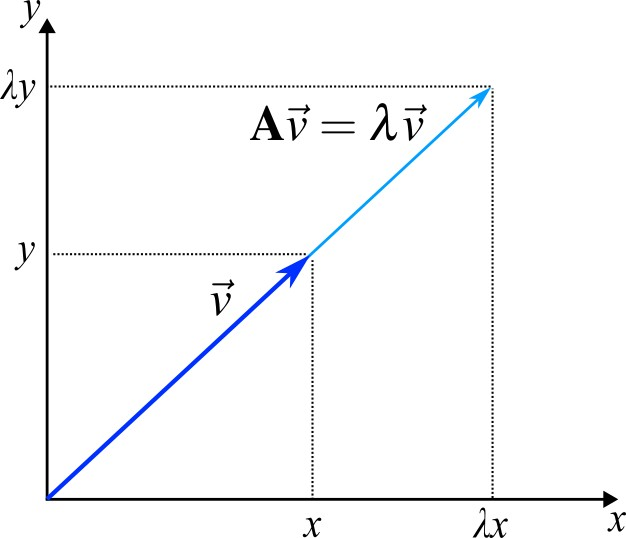
\includegraphics[width=3in]{../figures/eigenvalues}
			\caption{Matrix $\textbf{A}$ acts by stretching the vector $\vec{v}$, not changing its direction, so $\vec{v}$ is an eigenvector of $\textbf{A}$.}
			\label{fig:eigenvalues}
		\end{figure}
	
		The generalized eigenvalue problem is an important formulation for the study of vibrations and is written as 
		\begin{equation}
			\textbf{A}\textbf{v} = \vec{\lambda}\textbf{B}\textbf{v}
		\end{equation}	
		where $\textbf{A}$ and $\textbf{B}$ are real matrices. As written, this expression maps a general space $\textbf{A}$ into $\textbf{B}$ using $\vec{\lambda}$ and $\textbf{v}$. In the study of vibrations, the general generalized eigenvalue problem is used to link mass ($M$) and stiffness ($k$) matrices such that 
		\begin{equation}
			\textbf{K}\textbf{v} = \vec{\lambda}\textbf{M}\textbf{v}
		\end{equation}		
		
		%\rd{Need to add a discussion on normal, orthogonal, and orthonormal matrices.}	
		
	\end{review}	

	
	
	\subsubsection{Deriving the Eigenvalue-based Solution}
	 
	To derive an eigenvalue-based solution for calculating the natural frequencies and mode shapes in a computationally efficient way, we need to merge our mass and stiffness into one expression; termed the  mass normalized stiffness $\widetilde{K}$ matrix that we mathematically define later. First, let us consider that the vast majority of mass ($\textbf{M}$) and stiffness ($\textbf{K}$) matrices are symmetric and positive definite due to the physical meaning of these matrices. Therefore, $\textbf{M}$ can be factored into two terms using the Cholesky decomposition:
		\begin{equation}
			M=LL^{\text{T}}
		\end{equation}
	\begin{review}
	\textbf{Cholesky Decomposition} 

		\noindent The Cholesky decomposition of a real positive-definite matrix $A$ is a decomposition of the form:
		\begin{equation}
			\textbf{A}=\textbf{LL}^{\text{T}}
			\end{equation}
		where $\textbf{L}$ is the lower triangular matrix of $\textbf{A}$. 	A matrix is positive definite if the scalar $\textbf{x}^{\text{T}}A\textbf{x}$ is positive for any non-zero vector $x$ comprised of real numbers:
		\begin{equation}
			\textbf{x}^{\text{T}}\textbf{A}\textbf{x} > 0
		\end{equation}
	\end{review}	

		For the unique case diagonal mass matrices (all the mass values lie along the diagonal of the matrix) the Cholesky decomposition ($L$) is defined as:
		\begin{equation}
			L = M^{1/2} = \begin{bmatrix} \sqrt{m_1} & 0 \\  0  & \sqrt{m_2} \end{bmatrix} 
			\label{eq:Cholesky_lower_L}
		\end{equation}
		While a special case that is not always true, it is a commonly encountered mass matrix formulation due to the nature of mass matrices. Moreover, the example considered within this test all consists of a diagonal mass matrix. For the special case  diagonal mass matrices, equation~\ref{eq:Cholesky_lower_L} factors into:
		\begin{equation}
			M = M^{1/2}M^{1/2}
		\end{equation}
		Moreover, the inverse of the diagonal matrix ($M^{1/2}$) is denoted as $M^{-1/2}$ and defined as:
		\begin{equation}
			L^{-1} = M^{-1/2} = \begin{bmatrix} \frac{1}{\sqrt{m_1}} & 0 \\  0  & \frac{1}{\sqrt{m_2}} \end{bmatrix} 
		\end{equation}	
	
	
	Now, let us consider the previously derived EOM for an undamped 2-DOF system:
	\begin{equation}
	M\ddot{\vec{x}} + K\vec{x} =0
	\end{equation}
	This expression can be transformed into a symmetric eigenvalue problem, allowing us to leverage the strengths of symmetric eigenvalue mathematics and computer solvers. To solve the perform this transform, we set $\vec{x}=M^{-1/2}\vec{q}$ and multiply the equation by $M^{-1/2}$ such that the EOM becomes:
	\begin{equation}
	M^{-1/2}MM^{-1/2}\ddot{\vec{q}} + M^{-1/2}KM^{-1/2}\vec{q} =0
	\end{equation}
	As $M^{-1/2}MM^{-1/2}$ is equal to the identity matrix $I$ and defining $M^{-1/2}KM^{-1/2}$ as the mass normalized stiffness $\widetilde{K}$ yields the simplified expression:
	\begin{equation}
	I\ddot{\vec{q}} + \widetilde{K}\vec{q} =0
	\end{equation}
	where $\widetilde{K}=M^{-1/2}KM^{-1/2}$ is equivalent to the expression $k/m$ from the 1-DOF system as the are both mass-normalized stiffness values. 
	
	As before, a solution is found by assuming a solution, taking the derivatives of the solution, and substituting it into the EOM. Following these steps and assuming a solution of:
	\begin{equation}
	\vec{q} = \textbf{v}e^{j\omega t}
	\end{equation}
	where $\textbf{v}$ in an $n \times n$ matrix for a system with $n$ degrees of freedom. Adding this assumed solution to the EOM results in the form:
	\begin{equation}
	-\textbf{v} \omega^2 e^{j\omega t} + \widetilde{K}\textbf{v}e^{j\omega t} =0
	\end{equation}
	driving out the nonzero scaler $e^{j\omega t}$ and rearranging the above expression results in:
	\begin{equation}
	\widetilde{K}\textbf{v} =  \omega^2 \textbf{v}
	\end{equation}
	Knowing that $\textbf{v}\neq0$, as a matrix of zeros would mean no motion is present in the system, this equation can be expressed in a typical eigenvalue formulation:
	\begin{equation}
	\widetilde{K}\textbf{v} =  \lambda \textbf{v}
	\label{eq:eigenvalue_problem}
	\end{equation}
	where $\textbf{v}$ is a column matrix made up of the eigenvectors ($\textbf{v} = [v_1, \; v_1, \; \cdots, \; v_n ]$) and 
	$\lambda$ is a square matrix with eigenvalues on the diagonal. As $\widetilde{K}$ is symmetric, this is a symmetric eigenvalue problem. 
	
	An important attribute of eigenvectors to note is that the eigenvectors only encode information about the direction of the transformation while information on the magnitude is captured by the eigenvalue. Therefore, different values within an eigenvector may be used to represent the same direction.  A challenge for the entry-level practitioner is that different software systems may return different eigenvectors for the same problem. For example, MATLAB\protect\footnotemark[1] returns eigenvectors such that the 2-norm of each is 1. However, when solved symbolically\protect\footnotemark[2] non-normalized eigenvectors are returned. Various other engineering-focused applications may return normalized or non-normalized eigenvectors\protect\footnotemark[3]. Therefore, it is helpful for practitioners to normalize computed eigenvectors to unit norm eigenvectors to allow for comparison between different computational tools. 
	

	\footnotetext[1]{MATLAB 2023a {\ttfamily{}eig} function.} 
	\footnotetext[2]{MATLAB 2023a Symbolic Math Toolbox.} 
	\footnotetext[3]{LAPACK.} 	
	
	
		\begin{review}	
		\textbf{Vector Norms} 
		
	\noindent The Euclidean norm of a vector (also termed as 2-norm, Euclidean length or the vector magnitude) is defined as:
	\begin{equation}
	||\textbf{v}|| = \sqrt{\sum_{i=1}^{n}(v_i^2)} = \sqrt{\textbf{v}^{\text{T}}\textbf{v}}
	\end{equation} 
	If $||\textbf{v}|| = 1$ it is a ``unit norm''. If $||\textbf{v}||$ is not a a unit norm vector, in can be converted to one in by applying a scalar $\alpha$ such that such that $\alpha\textbf{v}=1$. In general, a nonzero vector $\textbf{v}$ of any length can be normalized to $\textbf{v}_\text{normalized}$ using the following expression:
		\begin{equation}
		\textbf{v}_\text{normalized} = \frac{1}{\sqrt{\textbf{v}^{\text{T}}\textbf{v}} } \textbf{v}
		\end{equation}
	\end{review}	

	
	
	 
	
	\begin{example}
	\label{ex:vector_normalizeation}

	\textbf{Normalizing Vectors}

	\noindent Normalize the Eigenvector $\vec{v}_1=[1/3 \hspace{1ex} 1]^\text{T}$. \\
		
	\noindent \textbf{Solution:} 
	
	\noindent First, let's check the Euclidean norm of $\vec{v}_1$, this is $\sqrt{1^2+1/3^2} = \sqrt{1.11} = 1.05$; therefore, the unit vector is not unit norm.
	
	To normalize the vector $\vec{v}_1$, a scalar ($\alpha$) is calculated to make $\alpha\textbf{v}=1$.  Therefore, following the definition of an orthogonal vector:
	\begin{equation}
	(\alpha \vec{v}_1)^\text{T}(\alpha \vec{v}_1) = 1
	\end{equation}
	or:
	\begin{equation}
	\alpha [1/3 \hspace{1ex} 1]\alpha  \begin{bmatrix} \frac{1}{3}\\  1 \end{bmatrix}  = \alpha^2(1/9+1) = 1
	\end{equation}
	Therefore, $\alpha=3/\sqrt{10}$. Resulting in a normalized unit vector of
	\begin{equation}
		\vec{v}_{1-\text{normalized}} = \alpha\vec{v}_1= \begin{bmatrix} \frac{1}{\sqrt{10}}\\  \frac{3}{\sqrt{10}} \end{bmatrix}
		\end{equation}
		 as $\sqrt{(1/\sqrt{10})^2 + (3/\sqrt{10})^2} =1$
	
	\end{example}	
	
	%Given that we set $\vec{x}=M^{-1/2}\vec{q}$, the eigenvectors are not a direct representation of the mode shapes. 
	%To develop a link between the  we first need to normalize the lengths of the eigenvectors obtained by solving equation \ref{eq:eigenvalue_problem} to that of a unit vector.
		
	Eigenvalues from the EOM are equal to $\omega^2$. Or more importantly, $\omega_i = \sqrt{\lambda_i}$. 
	Moreover, we can relate the eigenvectors to the modes shapes by a factor of the mass matrix:
	\begin{equation}
	\vec{u}_1 = M^{-1/2}\vec{v}_1
	\label{eq:modeshape_to_eigenvector}
	\end{equation}
	The important thing to remember is that the natural frequencies are the square root of the eigenvalues and the mode shapes are related to the eigenvectors through the mass matrix. Expanding on equation \ref{eq:modeshape_to_eigenvector}, one can go from the mode shapes to the eigenvector through:
	\begin{equation}
	\vec{v}_1 = M^{1/2}\vec{u}_1
	\end{equation}
	therefore, it can be seen that the eigenvectors and mode shapes are related through the mass normalization process. 
		
	

	
	
	\pagebreak
	\begin{example}

	\noindent \textbf{Calculating Eigenvalue-based Solutions for System Dynamics}  

	\noindent Consider the system presented in example \ref{ex:2-DOF} and repeated below where $m_1$=9~kg, $m_2$=1~kg, $k_1$ = 24~N/m, and $k_2$ = 3~N/m with the initial conditions $x_{10}=1$~mm, $v_{10}=0$~mm/s, $x_{20}=0$~mm, and $v_{20}=0$~mm/s. Calculate the natural frequencies and the mode shapes using the eigenvalue solution. 
	\begin{figure}[H]
		\centering
		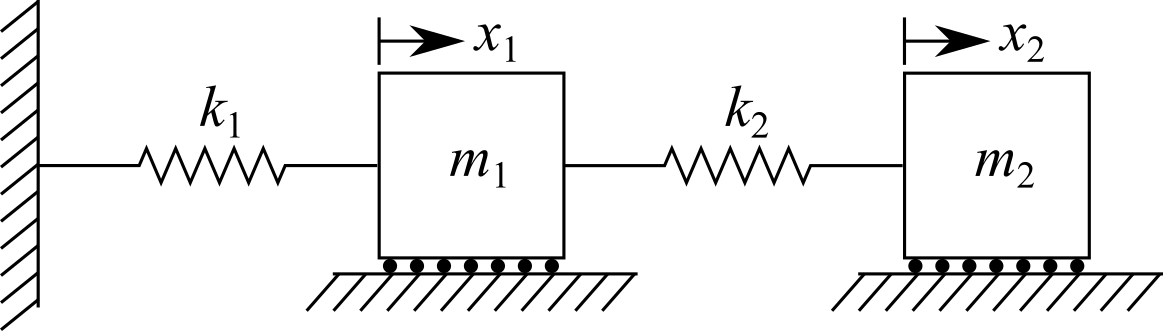
\includegraphics[]{../figures/2-DOF-spring_mass_horizontal.png}
		\caption{2-DOF system with two masses and two independent confidante systems $x_1$ and $x_2$.}
	\end{figure}
	
	
	
	
\noindent \textbf{Solution:}  

\noindent Writing the mass and stiffness matrix of the system as:
	
	\begin{equation}
		M = \begin{bmatrix} 9 & 0 \\  0  & 1 \end{bmatrix} 
	\end{equation}
	and 
	\begin{equation}
		 K = \begin{bmatrix} 27 & -3 \\    -3  & 3 \end{bmatrix}
	\end{equation}
	we can compute  $\widetilde{K}$ using the following expression:
	\begin{equation}
		 \widetilde{K}=M^{-1/2}KM^{-1/2}
	\end{equation}
	where $KM^{-1/2}$ is computed first to maintain symmetry. This results in:
	\begin{equation}
		 KM^{-1/2} =  \begin{bmatrix} 27 & -3 \\    -3  & 3 \end{bmatrix}  \begin{bmatrix} \frac{1}{3} & 0 \\    0  & 1 \end{bmatrix}= \begin{bmatrix} 9 & -3 \\    -1  & 3 \end{bmatrix}
	\end{equation}
	and:
	\begin{equation}
		  \widetilde{K}=M^{-1/2}KM^{-1/2} =  \begin{bmatrix} \frac{1}{3} & 0 \\    0  & 1 \end{bmatrix} \begin{bmatrix} 9 & -3 \\    -1  & 3 \end{bmatrix} =  \begin{bmatrix} 3 & -1\\  -1  & 3 \end{bmatrix} 
	\end{equation}
	Now a solution must be obtained for the eigenvalue problem:
	\begin{equation}
	\widetilde{K}\textbf{v} =  \lambda \textbf{v}
	\end{equation}
	
	While this can be obtained using computers for such a simple case it is more appropriate to solve this expression by had. Therefore, the above expression can be rewritten as:
	\begin{equation}
	(\widetilde{K} - \lambda I)\textbf{v} =  0
	\end{equation}
	However, as $\textbf{v} \neq 0$ the matrix must be singular, the determinant of the $(\widetilde{K} - \lambda I)$ matrix must equal zero. Or:
	\begin{equation}
	\det \begin{bmatrix} 3-\lambda & -1 \\    -1  & 3-\lambda \end{bmatrix}  =  0
	\end{equation}
	This can be expanded to the characteristic equation:
	\begin{equation}
	\lambda^2 -6\lambda + 8  =  0
	\end{equation}
	with the roots (eigenvalues):
	\begin{equation}
	\lambda_1 = 2\text{ and } \lambda_2 = 4
	\end{equation}
	Therefore, $\omega_1=\sqrt{2}$ and $\omega_2=2$. These are the same values computed in example \ref{ex:2-DOF}. The eigenvectors for $\lambda_1$ are computed as:
	\begin{equation}
	(\widetilde{K} - \lambda_1 I)\textbf{v} =  0
	\end{equation}
	or:
	\begin{equation}
	\begin{bmatrix} 3-2 & -1 \\    -1  & 3-2 \end{bmatrix} \begin{bmatrix} v_{11} \\ v_{21}  \end{bmatrix} =  \begin{bmatrix} 0 \\ 0  \end{bmatrix}
	\end{equation}
	This results in two dependent scalar equations:
	\begin{equation}
	v_{11} - v_{21} = 0 \text{ and } -v_{11} + v_{21} =0
	\end{equation}
	That show us that $v_{11} = v_{21}$ or $\vec{v}_1=[1 \hspace{1ex} 1]^\text{T}$. First we find that $\vec{v}_1$ is not a unit norm vector as $\sqrt{v_{21}^2+v_{21}^2}\ne1$. Therefore, let's apply a scalar $\alpha$ to normalize it to a unit vector. Using $(\alpha \vec{v}_1)^\text{T}(\alpha \vec{v}_1) = 1$ we obtain:
	\begin{equation}
	\alpha [1 \hspace{1ex} 1]\alpha  \begin{bmatrix} 1 \\  1 \end{bmatrix}  = \alpha^2(2) = 1
	\end{equation}
	or $\alpha = 1/\sqrt{2}$. This allows us to normalize the vector knowing $\alpha \vec{v}_1=1$, resulting in a normalized vector of:
	\begin{equation}
	\alpha \vec{v}_1=  \frac{1}{\sqrt{2}} \begin{bmatrix} 1 \\ 1 \end{bmatrix}  =  \begin{bmatrix} 0.71 \\ 0.71 \end{bmatrix} 
	\end{equation} 
	
	A similar process is followed for $\lambda_2=4$ that leads to the normalized vector 
	\begin{equation}
	\alpha \vec{v}_2=  \frac{1}{\sqrt{2}} \begin{bmatrix} -1 \\ 1 \end{bmatrix} =  \begin{bmatrix} -0.71 \\ 0.71 \end{bmatrix} 
	\end{equation} 
	Lastly, the normalized eigenvectors can be converted to mode shapes using $\textbf{u} = M^{-1/2}\textbf{v}$. Resulting in: 
	\begin{eqnarray}
	\vec{u}_1 =  \begin{bmatrix} \frac{1}{3} & 0  \\  0 & 1 \end{bmatrix}   \begin{bmatrix} 0.71 \\ 0.71 \end{bmatrix} =  \begin{bmatrix} 0.24 \\  0.71 \end{bmatrix}
	\end{eqnarray}
	and:
	\begin{eqnarray}
	\vec{u}_2 =  \begin{bmatrix} \frac{1}{3} & 0  \\  0 & 1 \end{bmatrix}   \begin{bmatrix} -0.71 \\  0.71 \end{bmatrix} =  \begin{bmatrix} -0.24 \\  0.71 \end{bmatrix}
	\end{eqnarray}
	While these mode shapes are correct, it is common practice to report them normalized with a maximum value of 1, therefore, $\vec{u}_1 = [1/3 \hspace{1ex} 1]$ and $\vec{u}_2 = [-1/3 \hspace{1ex} 1]$. While unit-normalization of the eigenvectors was not required in this example to obtain the right solution, it is good practice. Note that these are the same mode shape vectors as computed in example \ref{ex:2-DOF}.
	
	\end{example}
	

	
	
		\begin{example}
		\textbf{Eigenvalue Approach Solved using MATLAB}
		
		\begin{figure}[H]
			\centering
			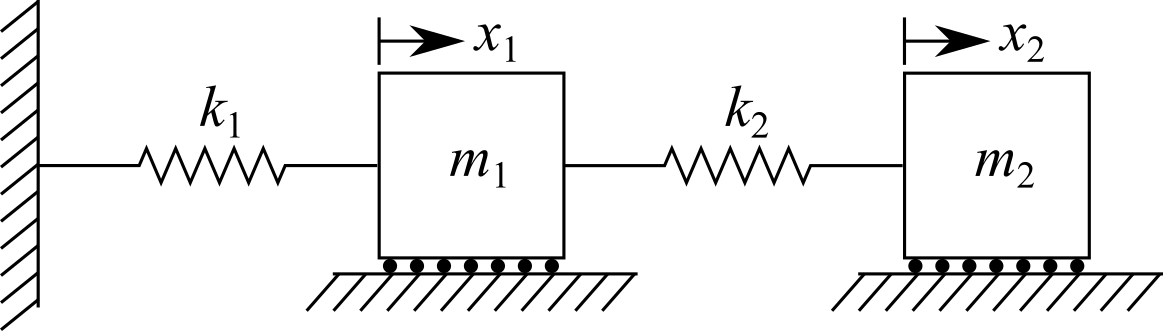
\includegraphics[]{../figures/2-DOF-spring_mass_horizontal.png}
			\caption{2-DOF system with two masses and two independent confidante systems $x_1$ and $x_2$.}
			\label{fig:2-DOF-spring_mass_horizontal_2}
		\end{figure}
		
		\noindent Using the Eigenvalue approach and MATLAB, determine the natural frequencies and mode shapes of the system shown in figure~\ref{fig:2-DOF-spring_mass_horizontal_2}, where $m_1$=9~kg, $m_2$=1~kg, $k_1$ = 24~N/m, and $k_2$ = 3~N/m with the initial conditions $x_{10}=1$~mm, $v_{10}=0$~mm/s, $x_{20}=0$~mm, and $v_{20}=0$~mm/s with the EOM expressed as: 
		\begin{eqnarray}
		  \begin{bmatrix} m_1 & 0  \\  0 & m_2 \end{bmatrix}\begin{bmatrix} \ddot{x_1} \\  \ddot{x_2} \end{bmatrix} + \begin{bmatrix} k_1+k_2 & -k_2  \\  -k_2 & k_2 \end{bmatrix}\begin{bmatrix} x_1 \\  x_2 \end{bmatrix} = \begin{bmatrix} 0 \\  0 \end{bmatrix}
		\end{eqnarray} \\
	
		\noindent \textbf{Solution:} 
	
	\noindent Using the eigenvalue method, the following MATLAB code will solve for the natural frequencies and mode shapes:
		
	\lstset{caption={MATLAB code to find the frequencies and mode shapes of a 2-DOF system.},
		label={lst:code},
		frame=lines,
		basicstyle=\ttfamily\footnotesize\bfseries}
		\begin{lstlisting}
% define the M and K matrix
M = [9 0; 0 1]
K = [24+3 -3; -3 3]

% build the M inverse square-root and mass normalized stiffness matrix 
M_inv_sqr = sqrt(inv(M))
K_mass_norm = M_inv_sqr*K*M_inv_sqr

% Using, K_mass_norm*v=lambda*v
[v,lambda] = eig(K_mass_norm)

% Solve for natural frequencies
omega_1 = sqrt(lambda(1,1))
omega_2 = sqrt(lambda(2,2))

% solve for the mode shapes
u_1 = M_inv_sqr*v(:,1)
u_2 = M_inv_sqr*v(:,2)
				\end{lstlisting}
		\noindent where $\omega_1$=1.41 rad/sec and  $\omega_2$=2 rad/sec while $\vec{u}_1 = [0.333 \; 1]$ and $\vec{u}_2 = [-0.333 \; 1]$.
		\end{example}
	
	
	
	
	%\section{forced vibration analysis}
	%5.6 in Gao has a section of mechanical impedance
	
	
	
	\subsection{Transfer-function Method}
	
	As in 1-DOF systems, transfer functions can be used to solve for the temporal response of 2-DOF systems under a variety of inputs. Again, the transfer function of a differential equation is defined as the ratio of the Laplace transform of the output (system response) to the Laplace transform of the input (forcing function). Moreover, the procedure for using the Laplace transform to solve the equations of motion is the same and follows three steps:
	\begin{enumerate}
		\item Take the Laplace transform of both sides of the EOM while treating the time derivatives symbolically.
		\item Solve for $X(s)$ in the obtained equation.
		\item Apply the inverse transform $x(t) = \Laplace{X(s)}^{-1}$.
	\end{enumerate}
	
	
	\begin{example}
	\textbf{2-DOF System Subjected to Impulse}
	
	\noindent Two masses are connected through a spring, as shown in figure~\ref{fig:2-DOF-spring_mass_free}. 
	\begin{figure}[H]
		\centering
		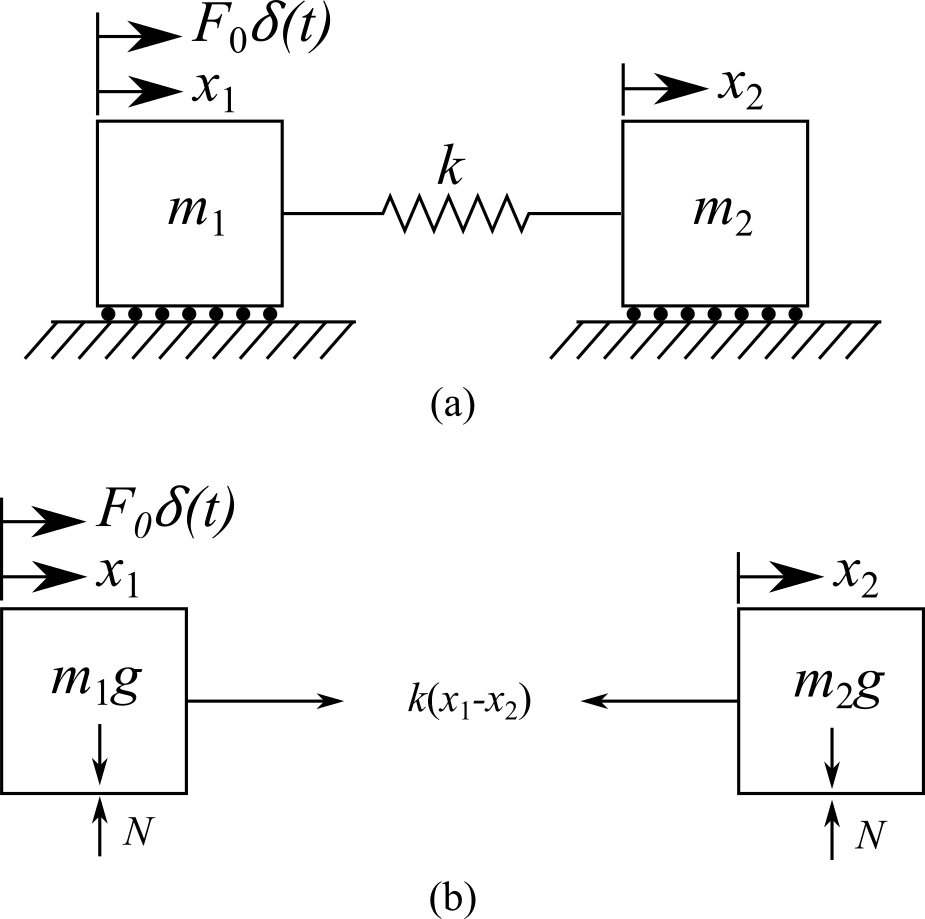
\includegraphics[]{../figures/2-DOF-spring_mass_free.png}
		\caption{2-DOF system subjected to an impulse showing: (a) system, and (b) FBD.}
		\label{fig:2-DOF-spring_mass_free}
	\end{figure}

\noindent \textbf{Solution:}

	\noindent Assuming that $x_1$ displaces more than $x_2$, the equations of motion are:
	\begin{eqnarray}
	m_1\ddot{x}_1 + k(x_1-x_2)  = F_0 \delta (t) \\
	m_2\ddot{x}_2 + k(x_2-x_1)  = 0  \nonumber
	\end{eqnarray}
	Taking the Laplace of both equations (step 1) yields:
	\begin{eqnarray}
	(m_1 s^2 +k)X_1(s) - k X_2(s) = F_0 \\
	-k X_1(s) + (m_2 s^2 + k) X_2(s) = 0  \nonumber
	\end{eqnarray}
	solving these two equations for $X_1$ and $X_2$ (step 2) results in:
	\begin{eqnarray}
	X_1(s) = \frac{F_0(m_2 s^2 +k)}{s^2 [m_1 m_2 s^2 + k (m_1 + m_2)]} \\
	X_2(s) = \frac{F_0 k}{s^2 [m_1 m_2 s^2 + k (m_1 + m_2)]} \nonumber
	\end{eqnarray}
	Using partial fractions, or a symbolic toolbox in MATLAB or Python, these expressions can be rewritten as:
	\begin{eqnarray}
	X_1(s) = \frac{F_0}{m_1 + m_2} \bigg( \frac{1}{s^2} + \frac{m_2}{\omega m_1} \frac{\omega}{s^2 + \omega^2} \bigg) \\
	X_2(s) = \frac{F_0}{m_1 + m_2} \bigg( \frac{1}{s^2} + \frac{1}{\omega} \frac{\omega}{s^2 + \omega^2} \bigg) \nonumber
	\end{eqnarray}
	where:
	\begin{equation}
	\omega^2 = k \bigg( \frac{1}{m_1} + \frac{1}{m_2} \bigg)
	\end{equation}
	Taking the inverse transform of the expressions for $X_1(s)$ and $X_2(s)$ (step 3) results in expressions in the time domain and yields:
	\begin{eqnarray}
	x_1(t) = \frac{F_0}{m_1 + m_2} \bigg( t + \frac{m_2}{\omega m_1} \sin (\omega t) \bigg) \\
	x_2(t) = \frac{F_0}{m_1 + m_2} \bigg( t + \frac{1}{\omega} \sin (\omega t) \bigg) \nonumber
	\end{eqnarray}
	Considering a system where $F_0=10$ N, $m_1=1000$~kg, $m_2=1000$~kg, and $k=1500$~N/m the temporal response is annotated in figure~\ref{fig:2_DOF_impact_example}. 
	
	
	\begin{figure}[H]
		\centering
		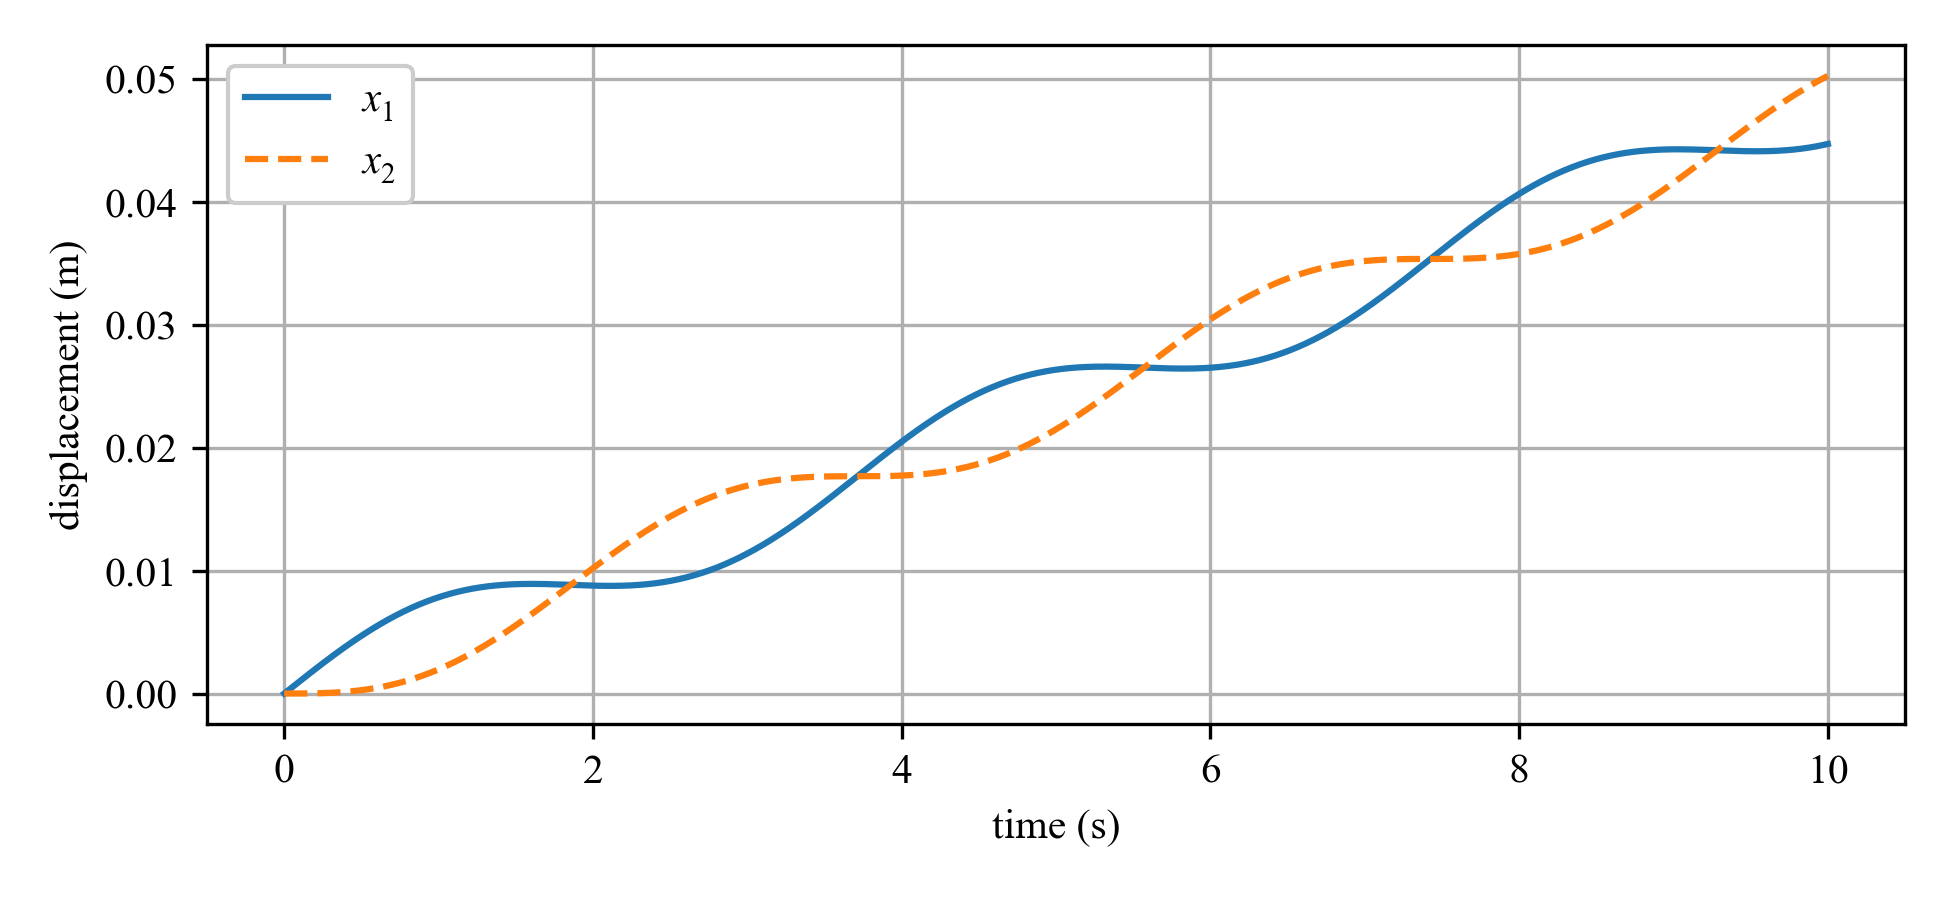
\includegraphics[width=\linewidth]{../figures/2_DOF_impact_example.png}
		\caption{Temporal response for the considered 2-DOF system subjected to an impact load.}
		\label{fig:2_DOF_impact_example}
	\end{figure}
	
	
	\end{example}
	
	
	% \subsection{Frequency Response Transfer Functions}
	
	%\rd{Rao ed 5.11, p 526}
	
	
	% \subsection{Computational Methods for 2-DOF Systems}
	
	

%%%%%%%%%%%%%%%%%%%%%%%%%%%%%%%%%%%%%%%%%%%%%%%%%%%%%%%%%%%%%%%%%%%%%%%%%%%%%	
%	What follows here is poorly developed matlab examples that should be deleted/re-worked
%%%%%%%%%%%%%%%%%%%%%%%%%%%%%%%%%%%%%%%%%%%%%%%%%%%%%%%%%%%%%%%%%%%%%%%%%%%%%
%	\begin{example}
%	\textbf{Roots of Quadratic Equation} \\
%Using MATLAB, find the roots of following quadratic equation.
%\begin{equation}
%x^4 -8x +12 = 0
%\end{equation} \\
%
%\noindent \textbf{Solution:} 
%
%\lstset{%
%	caption={MATLAB code for time series responses of 1\textsuperscript{st} order system.},
%	basicstyle=\ttfamily\footnotesize\bfseries,
%	frame=tb,
%}
%\begin{lstlisting}
%% for the function f(x) = x^4 -8x +12 =0
%roots([1 0 0 -8 12]) 
%\end{lstlisting}
%	\end{example}
%	

%	
	
	%\subsubsection{Python}
	
	
	
	
	\subsection{Multiple Degrees of Freedom}
	
	This chapter introduces methodologies for the solving of systems with more than 2-DOF. As shown in Chapter 5, 2-DOF systems can be solved analytically using 2 EOM coupled through their mode shapes. However, these methods become tedious when extended to systems with damping or even beyond the 2-DOF system.
	
	
	
	\begin{example}
	\textbf{Multiple Mode Shapes}
	
	
	
	\begin{figure}[H]
		\centering
		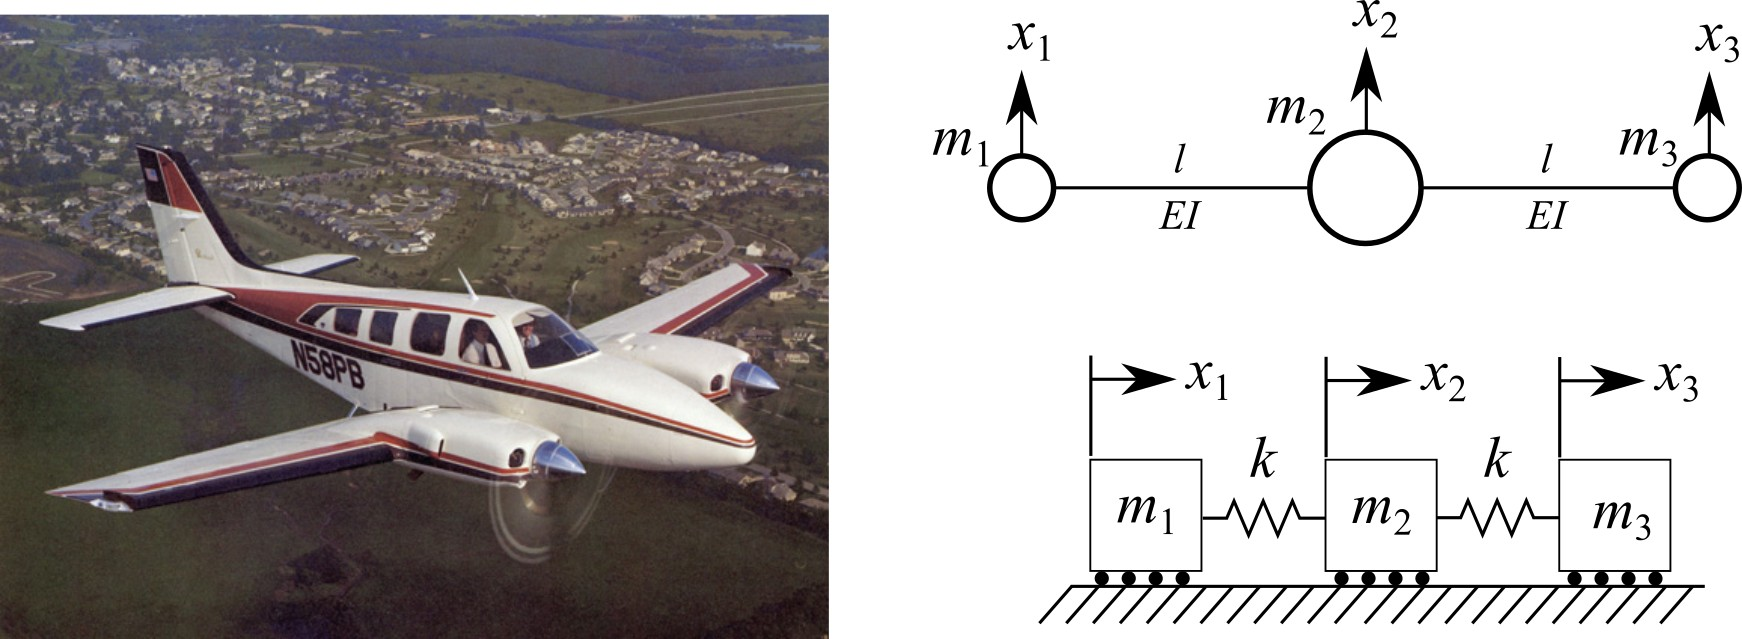
\includegraphics[width=\linewidth]{../figures/mode_shape_aiplane_example}
		\caption{A Beechcraft Baron in flight\protect\footnotemark[1] along with the Free-Free 3-DOF model simplified as a mass-spring model.}
		\label{fig:mode_shape_aiplane_example}
	\end{figure}
	\footnotetext[1]{``A Beechcraft Baron 58 in flight'' by San Diego Air \& Space Museum Archives, Public Domain.}  
	
	\noindent Modeling the vibrations of a twin-engine airplane as a three-degree-of-freedom system can be done as shown in figure~\ref{fig:mode_shape_aiplane_example} where the fuselage is a center mass, and the engines are point masses suspended by cantilevers from the center mass. The stiffness of the wing corresponds to the modulus of the wing $E$ and its moment of inertia $I$. 
	Assuming that $m_1=m_3=1m$, $m_2=3m$, and $k=\frac{3EI}{l}$, the EOM can be written as:
	
	\begin{equation}
		  m\begin{bmatrix} 1 & 0 & 0 \\    0  & 3 & 0 \\ 0  & 0 & 1 \end{bmatrix} \begin{bmatrix} \ddot{x}_1 \\    \ddot{x}_2 \\    \ddot{x}_3  \end{bmatrix} + \frac{EI}{l} \begin{bmatrix} 3 & -3 & 0 \\  -3  & 6 & -3 \\  0  & -3 & 3 \end{bmatrix} \begin{bmatrix} x_1 \\    x_2 \\    x_3 \end{bmatrix} = \begin{bmatrix} 0 \\  0 \\ 0 \end{bmatrix} 
	\end{equation}
	calculate the natural frequencies and mode shapes of the system and plot the mode shapes in relation to the considered Beechcraft Baron.
	

	\noindent \textbf{Solution using the mass normalized stiffness matrix $\tilde{K}$:}

	
	\noindent 	Solving for the modes shapes using the  mass normalized stiffness matrix $\tilde{K}$ requires solving for $M^{-1/2}$ and $\tilde{K}$ such that:
	\begin{equation}
		  M^{-1/2} = \begin{bmatrix} 1 & 0 & 0 \\    0  & 0.577 & 0 \\ 0  & 0 & 1 \end{bmatrix}
	\end{equation}
	\begin{equation}
		   \tilde{K} = M^{-1/2} K M^{-1/2} = \frac{3EI}{l} \begin{bmatrix} 3 & -1.732 & 0 \\  -1.732  & 2 & -1.732 \\  0  & -1.732 & 3 \end{bmatrix} 
	\end{equation}
	Then, the eigenvalue problem, formulated as:
	\begin{equation}
	\tilde{K} \textbf{v} = \lambda \textbf{v}
	\end{equation}
	is solved for the eigenvalues and normalized eigenvectors using a computer, resulting in:
	\begin{equation}
	\lambda_1 = 0, \; \; \lambda_2 = 1.73, \; \; \lambda_3 = 2.23
	\end{equation}
	\begin{equation}
	\vec{v}_1 = \begin{bmatrix} 0.447 \\    0.775 \\    0.447  \end{bmatrix}, \; \; \vec{v}_2 = \begin{bmatrix} -0.707 \\    0.0 \\    0.707 \end{bmatrix}, \; \; \vec{v}_3 = \begin{bmatrix} 0.548 \\    -0.632 \\    0.548  \end{bmatrix}
	\end{equation}
	When the eigenvalue problem is solved using the mass normalized stiffness matrix $\tilde{K}$ the natural frequencies are $\omega_i = \sqrt{\lambda_i}$ while the mode shapes are derived from the eigenvectors as $\vec{u}=M^{-1/2}\vec{v}$. This results in:
	\begin{equation}
	\omega_1 = 0  \text{ rad/sec}, \; \; \omega_2 = 1.414 \text{ rad/sec}, \; \; \omega_3 = 1.826  \text{ rad/sec}
	\end{equation}
	\begin{equation}
	\vec{u}_1 = \begin{bmatrix} 0.447 \\   0.447 \\    0.447 \end{bmatrix}, \; \; \vec{u}_2 = \begin{bmatrix} -0.707 \\    0.0 \\    0.707 \end{bmatrix}, \; \; \vec{u}_3 = \begin{bmatrix} 0.548 \\    -0.365 \\    0.548  \end{bmatrix}
	\end{equation}
	Next, normalizing the mode shapes by the max of the vector results in:
	\begin{equation}
	\vec{u}_1 = \begin{bmatrix} 1 \\    1 \\    1  \end{bmatrix}, \; \; \vec{u}_2 = \begin{bmatrix} -1 \\    0 \\    1 \end{bmatrix}, \; \; \vec{u}_3 = \begin{bmatrix} 1 \\    -0.667 \\    1  \end{bmatrix}
	\end{equation}
	these mode shapes can than be plotted as:
	\begin{figure}[H]
		\centering
		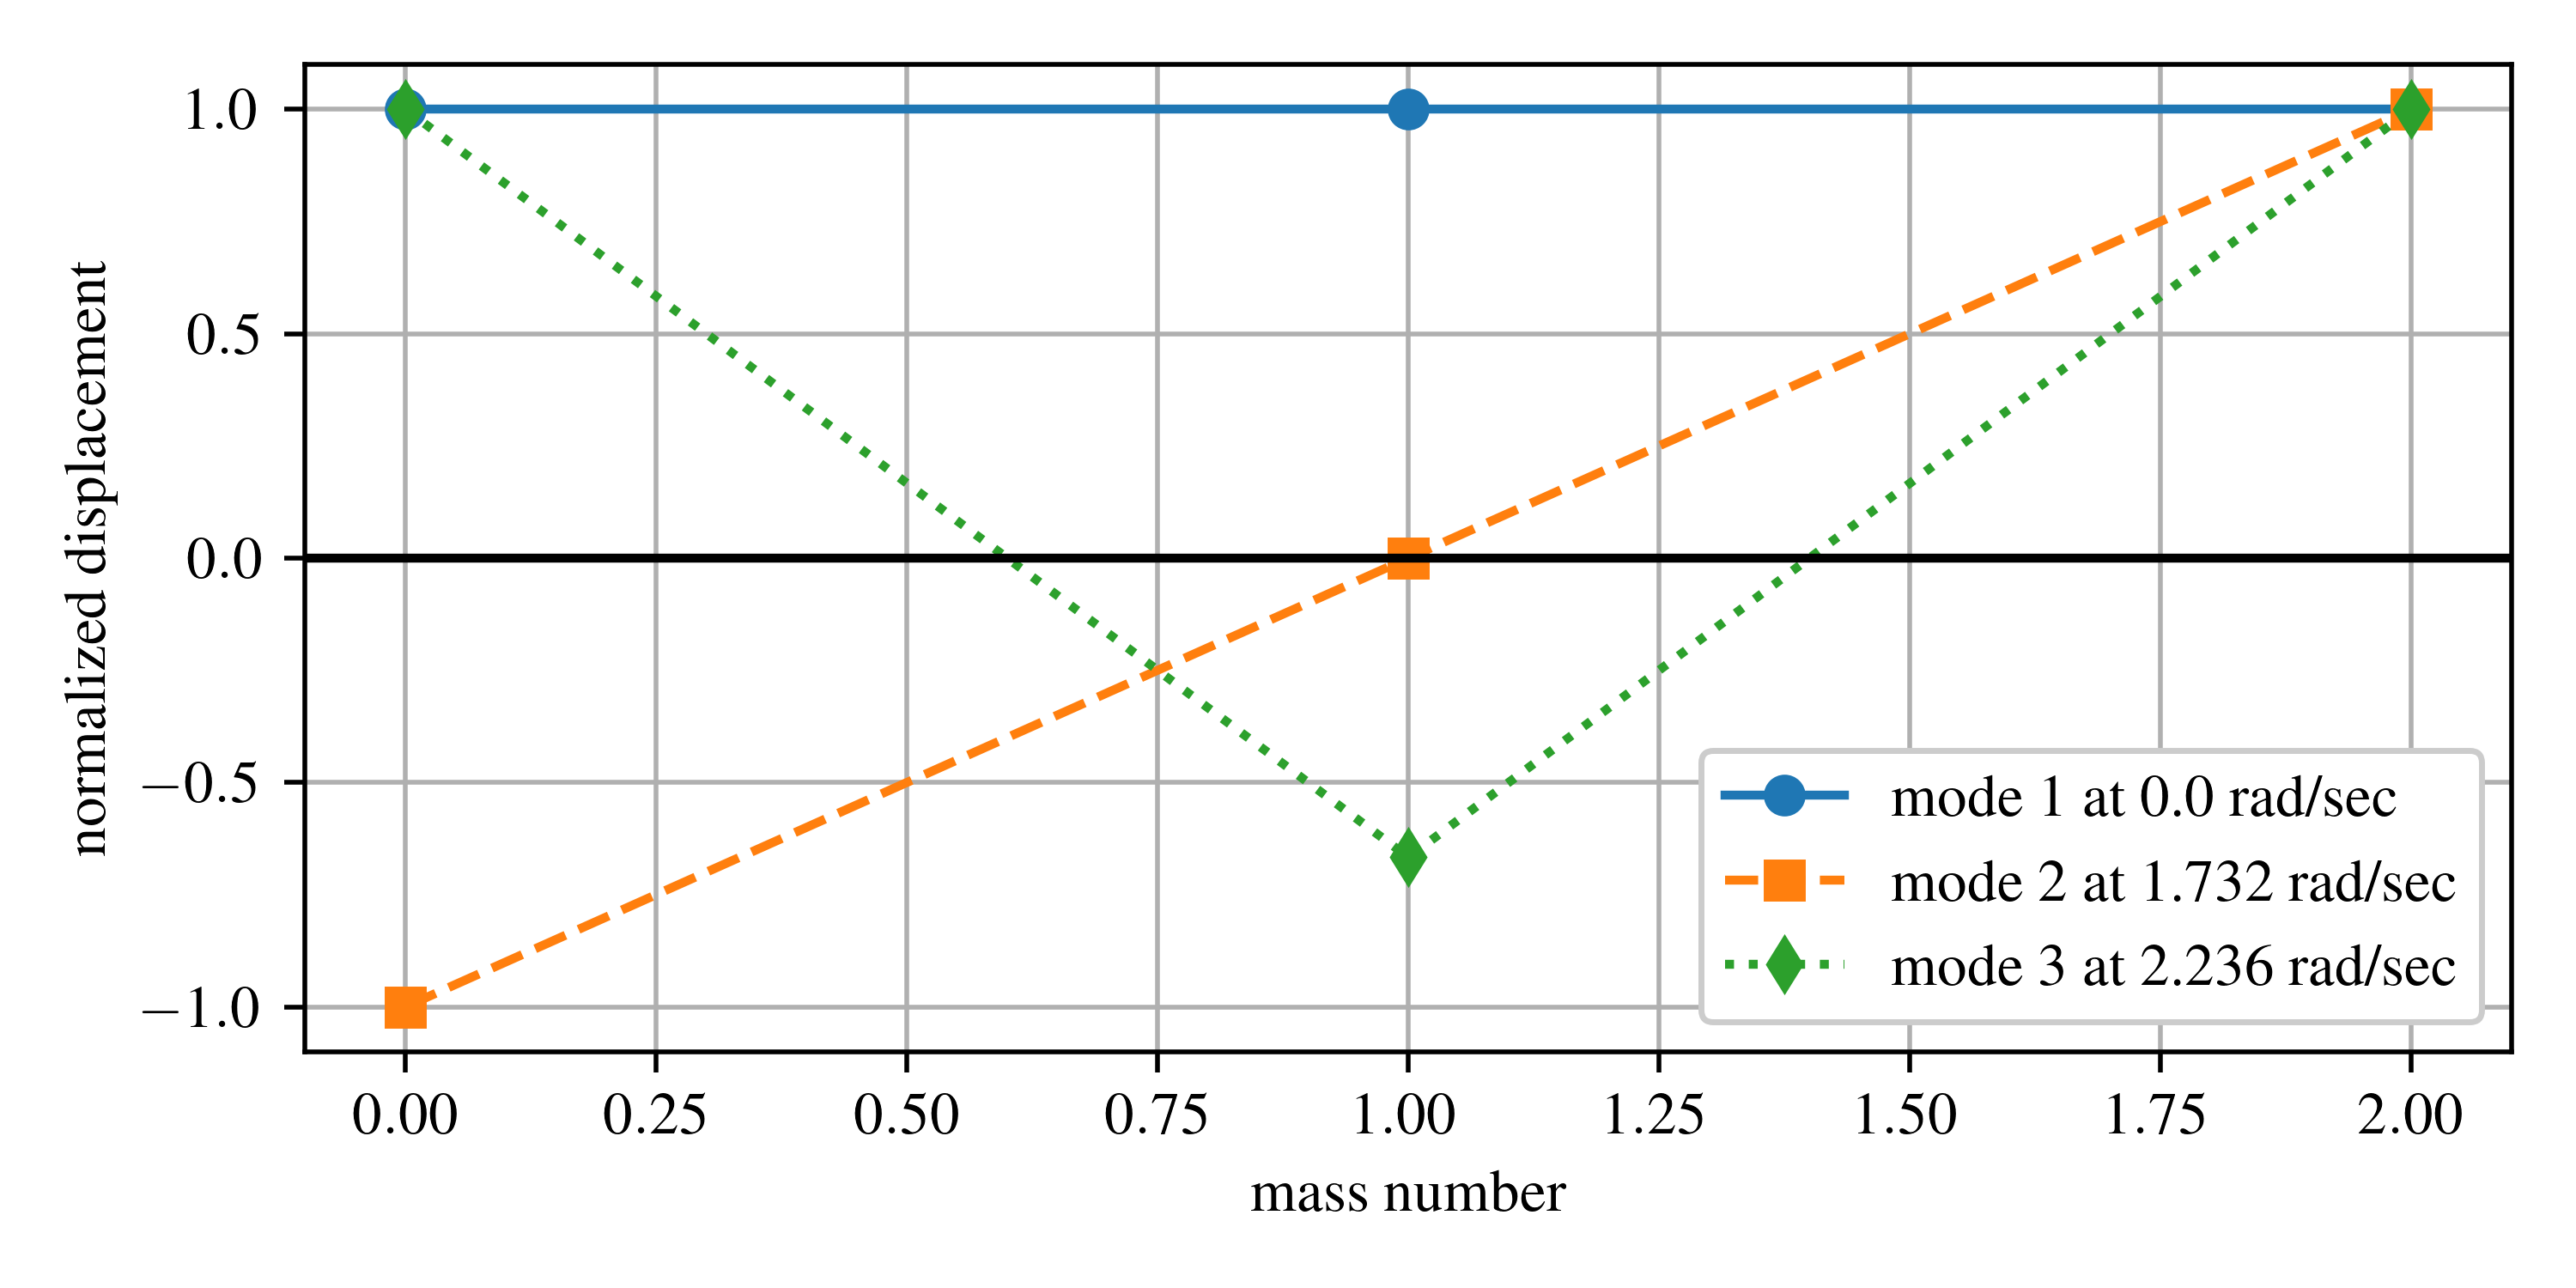
\includegraphics[width=\linewidth]{../figures/mode_shape_aiplane_example_normalized_stiffness.png}
		\caption{The unit vector normalized displacement of the mode shapes solved for using the mass normalized stiffness matrix $\tilde{K}$.}
		\label{fig:mode_shape_aiplane_example_normalized_stiffness}
	\end{figure}
	
	\noindent \textbf{Solution using the generalized eigenvalue approach:}

	\noindent The mode shapes can also be solved for using the generalized eigenvalue approach where the eigenvalue problem is written as:
	\begin{equation}
	\textbf{K}\textbf{v} = \vec{\lambda}\textbf{M}\textbf{v}
	\end{equation}
	solving for the eigenvalues and eigenvectors yields:
	\begin{equation}
	\lambda_1 = 0, \; \; \lambda_2 = 1.73, \; \; \lambda_3 = 2.23
	\end{equation}
	\begin{equation}
	v_1 = \begin{bmatrix} -0.577 \\    -0.577 \\   -0.577  \end{bmatrix}, \; \; v_2 = \begin{bmatrix} 0.707 \\    0.0 \\    -0.707 \end{bmatrix}, \; \; v_3 = \begin{bmatrix} 0.639 \\    -0.426 \\    0.639 \end{bmatrix}
	\end{equation}
	Note that the eigenvalues are the same as those solved for using the normalized stiffness matrix approach while the eigenvectors appear to be different (mode 2). software tools and computing languages do not all follow the same standards in terms of returning eigenvectors as the information stored in the eigenvectors is just the direction of the transform. However, mode 2 reported here is still correct as only the shape of the eigenvalue matters.
	
	\begin{figure}[H]
		\centering
		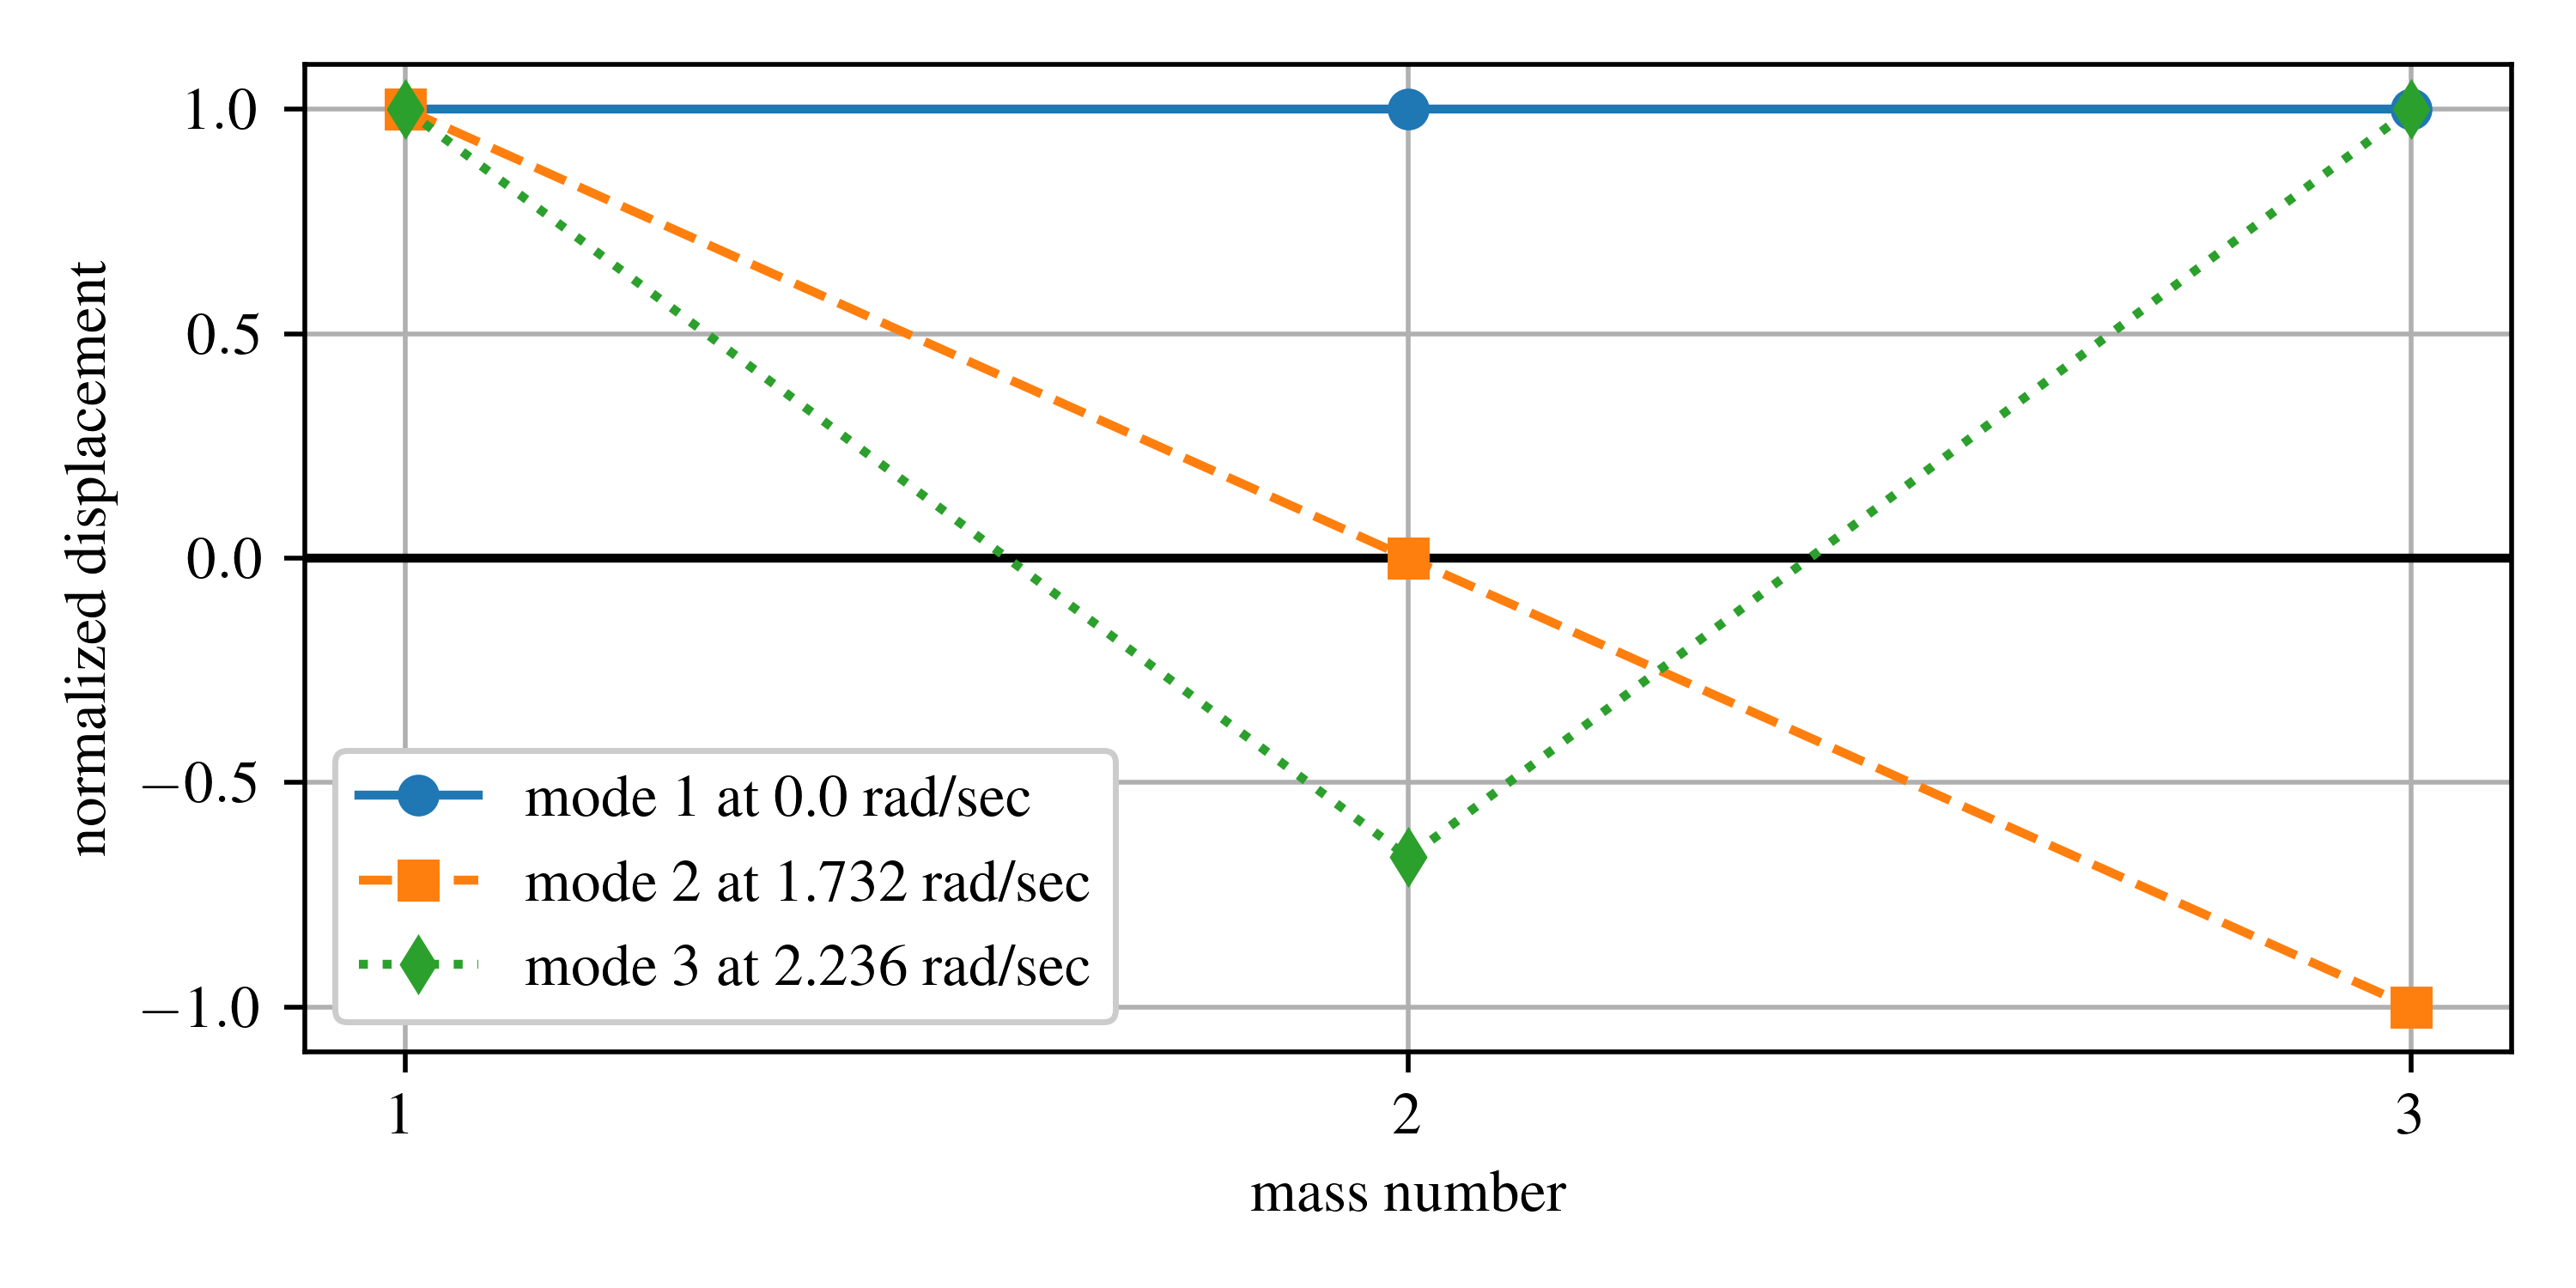
\includegraphics[width=\linewidth]{../figures/mode_shape_aiplane_example_generalized_eigenvalue.png}
		\caption{The unit vector normalized displacement of the mode shapes solved for using the generalized eigenvalue approach.}
		\label{fig:mode_shape_aiplane_example_generalized_eigenvalue}
	\end{figure}

	\end{example}
	
	
	
	
	\subsection{Modal Analysis}
	
	% Inman has S defined as a "modal matrix" and a "matrix of mode shapes", I belive his definition of S = M^(-1/2)P as a "matrix of mode shapes" is correct in the context of how I use it here. 
	
	% This math more closely lines up with Rao 6th edition section 6.14.
	
	Modal analysis is the study of a system's dynamic properties and is done in the frequency domain. Consider a system with $n$ degrees of motion, modal analysis allows for the uncoupling of the EOM into $n$ single-degree-of-freedom system (represented as 2$^{\text{nd}}$-order DOF systems) where the displacements of the masses are expressed as the linear summations of the normal modes of the system. If every mode shape is considered, the solution is equivalent to the solution obtained from the original $n^{\text{th}}$-degree-of-freedom system. 
	
	Consider the generic multidegree-of-freedom system under external forces, expressed as:
	
	
	\begin{equation}
	M \ddot{\vec{x}} + K\vec{x} = \vec{F}
	\end{equation}
	
	
	\noindent where damping is not considered and the vector $\vec{F}$ is a set of deterministic inputs. To expand this equation by modal analysis, the eigenvalue problem must first be solved. The generalized eigenvalue problem is written at: 
	
	\begin{equation}
	\lambda M \textbf{v} = K \textbf{v}
	\label{eq:generiq_MDOF_system}
	\end{equation}
	
	For the $n^{\text{th}}$-degree-of-freedom, the generalized eigenvalue problem can be simplified to: 
	\begin{equation}
	\omega_i^2 M \vec{v}_i = K  \vec{v}_i
	\end{equation}
	Considering that the total displacement of the system, expressed as $\vec{x}(t)$ , is the summation of the displacement of each of the noncontributing modes; assuming a linear system, the temporal response of the system can be written as:
	\begin{eqnarray}
	\vec{x}(t) = q_1(t) \vec{v}_1 + q_2(t) \vec{v}_2 + q_3(t) \vec{v}_3 + \cdots + q_n(t) \vec{v}_n
	\label{eq:combination_of_modes}
	\end{eqnarray}
	\noindent where the time-dependent generalized scalars $q_1(t), \; q_1(t), \; \cdots, \; q_1(t)$ are the modal participation coefficients (also called principal coordinates). Defining the modal matrix $P$ as: 
	\begin{equation}
	P = [ \vec{v}_1 \;  \vec{v}_2 \;  \vec{v}_3 \; \cdots \; \vec{v}_n]
	\end{equation}
	where $\vec{v}_1 = M^{-1/2}u_1$ and are the orthonormal eigenvectors of $\tilde{K}$ (i.e. the mass normalized eigenvectors) and not the eigenvectors of the original system formation shown in equation~\ref{eq:generiq_MDOF_system}. Note that the modal matrix is made of of the eigenvectors of $\tilde{K}$ and not the mode shapes of the system; for context see review~\ref{review:modal_matirx}.

		\begin{review}	
		\label{review:modal_matirx}
		\textbf{Modal Matrix} 

		\noindent A modal matrix is a mathematical concept taken from linear algebra and not specific to vibrations or structural dynamics. This is why the modal matrix does not contain the modes of the system but rather eigenvectors. 
			
			From linear algebra, the modal matrix $B$ for the matrix $A$ is a matrix of size $n \times n$ consisting of the eigenvectors of $A$ as columns in $B$. It is used in the definition of matrix similarity such that 
			\begin{equation}
			C = B^{-1}AB
			\end{equation}
			where $C$ is a $n \times n$ diagonal matrix with the eigenvalues of $A$ on the main diagonal (zeros elsewhere). $D$ is the spectral matrix of $A$. The eigenvalues must appear in the diagonal (top-left to bottom-right in the same order as their corresponding eigenvectors are arranged in $B$ (column-wise left to right).			
		\end{review}	
	
	
		
	The linear combination of the normal modes (equation~\ref{eq:combination_of_modes}) can be more concisely written as:
	\begin{equation}
	\vec{x}(t) = P\vec{q}(t)
	\end{equation}
	where $\vec{q}(t) = [q_1 \; \; q_2 \; \; q_3 \cdots q_n]^{\text{T}}$. Next, the relationship that relates the physical space to the modal space for the acceleration component is written as:
	\begin{equation}
	\ddot{\vec{x}}(t) = P\ddot{\vec{q}}(t)
	\end{equation}
	combining these two terms results in the EOM that can be written as:
	\begin{equation}
	M P\ddot{\vec{q}}(t) + KP\vec{q}(t) = \vec{F}
	\end{equation}
	To convert the EOM into the standard form, first the $P^{\text{T}}$ is multiplied through the equation as:
	\begin{equation}
	P^{\text{T}} M P\ddot{\vec{q}}(t) + P^{\text{T}} K P\vec{q}(t) = P^{\text{T}} \vec{F}
	\end{equation}
	If the modes are normalized, the following is true: 
	%%%%%%%%%%%%%%%%%%%%%%%%%%%%%%%%%%%%%%%%%%%%%%%%%%%%%%%%%
	%\todo{Should this be $\widetilde{K}$?} I am not sure how the normalization works here. 
	%%%%%%%%%%%%%%%%%%%%%%%%%%%%%%%%%%%%%%%%%%%%%%%%%%%%%%%%%
	\begin{equation}
	P^{\text{T}} M P = I
	\label{eq:modes_normalized}
	\end{equation}
	where $I$ is the identity matrix and 
	\begin{equation}
	P^{\text{T}} K P = \begin{bmatrix} \nwarrow & 0 & 0 \\  0  & \omega^2 & 0 \\  0  & 0 & \searrow \end{bmatrix}
	\end{equation}
	
	Next we define $\vec{Q}(t)$ as vector of generalized forces in the modal space such that $\vec{Q}(t) = P^{\text{T}}\vec{F}$. This results in a EOM in the modal space expressed as:
	\begin{equation}
	\ddot{\vec{q}}(t) +  \begin{bmatrix} \nwarrow & 0 & 0 \\  0  & \omega^2 & 0 \\  0  & 0 & \searrow \end{bmatrix} \vec{q}(t) = \vec{Q}(t)
	\end{equation}
	For a system with $n$ degrees of freedom, this equation can be broken down into:
	\begin{equation}
	\ddot{q}_i(t) + \omega_i^2 q_i (t) =  Q_i(t), \; \; i=1, \; 2, \; \cdots, \;n
	\end{equation}
	This expression is the same ODE that we have solved multiple times in this text. Therefore, we know the solution to be:
	\begin{equation}
	q_i(t) = q_{i0} \cos(\omega_i t) +  \frac{\dot{q}_{i0}}{\omega_i} \sin( \omega_i t)
	\end{equation}
	Lastly, to solve for a solution in the modal space, the initial conditions that were given in the physical space must be converted to the modal space. This can be done by generalizing the velocities in terms of the modal matrix:
	\begin{equation}
	\vec{q}(0) = P^\text{T} M \vec{x}(0)
	\end{equation}
	\begin{equation}
	\dot{\vec{q}}(0) = P^\text{T} M \vec{v}(0)
	\end{equation}
	
	
	%\todo{test}
	
	\begin{example}
	\textbf{Free Vibration Response}
	
	\noindent Solve for the free vibration response of the 2-DOF presented in figure~\ref{fig:2-DOF-spring_mass_horizontal_double_wall} using modal analysis. Show the temporal response for the entire system for its first 20 seconds using the full modal reconstruction and the reconstruction truncated to just include the first mode. Also, plot the variations in the modal participation coefficients through time. Apply the parameters, $f_1 = 0$ N, $f_2 = 0$ N, $m_1 = 10$~kg, $m_2 = 1$~kg, $k_1 = 30$~N/m, $k_2 = 5$~N/m, $k_3 = 1$~N/m, $x_1(0) = 1$~mm, $x_2(0) = 0$~mm, $v_1(0) = 0$~mm/s, and $v_2(0) = 0$~mm/s.
	
	\begin{figure}[H]
		\centering
		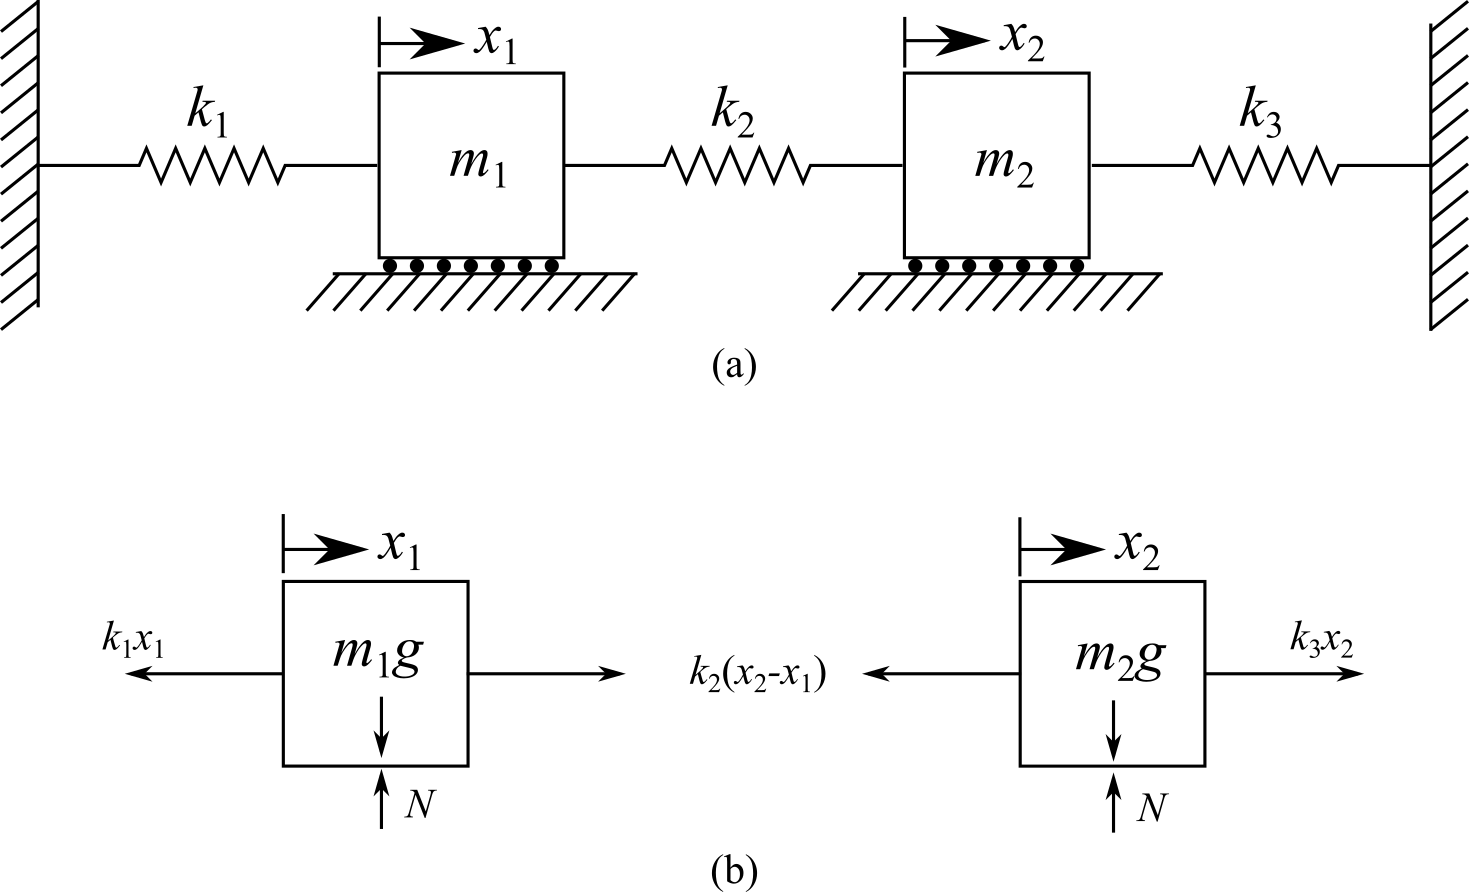
\includegraphics[]{../figures/2-DOF-spring_mass_horizontal_double_wall.png}
		\caption{Forced 2-DOF damped system showing: (a) system, and (b) FBD.}
		\label{fig:2-DOF-spring_mass_horizontal_double_wall}
	\end{figure}

\noindent \textbf{Solution:} 

\noindent The equations of motion that couple the system are:
	\begin{eqnarray}
	m_1\ddot{x}_1 + (k_1+k_2)x_1 - k_2x_2 = 0 \\
	m_2\ddot{x}_2 + (k_2+k_3)x_2 - k_2x_1 = 0 \nonumber
	\end{eqnarray}
	In matrix form, these become:
	
	\begin{equation}
		  \begin{bmatrix} m_1 & 0 \\    0  & m_2 \end{bmatrix} \begin{bmatrix} \ddot{x}_1 \\    \ddot{x}_2  \end{bmatrix} + \begin{bmatrix} k_1 + k_2 & -k_2 \\  -k_2  & k_2 + k_3 \end{bmatrix} \begin{bmatrix} x_1 \\    x_2  \end{bmatrix} = \begin{bmatrix} 0 \\  0  \end{bmatrix} 
	\end{equation}
	\begin{equation}
		  \vec{x}(0) = \begin{bmatrix} 1 \\  0 \end{bmatrix},\; \; \vec{v}(0) = \begin{bmatrix} 0 \\  0 \end{bmatrix} \nonumber
	\end{equation}
	The natural frequencies and mode shapes can then be obtained by solving the eigenvalue problem. Setting up the generalized eigenvalue problem: %
	
	%\rd{look at symmetric M and K matrices} %\rd{these are symmetric M and K matrices so I don't know why $\tilde{K}$ does not work in a normal eigenvalue problem. Maybe norms of vectors? It is not simple scaling. This example is based off of Rao 6.16 6ed} \rd{I think it has to do with solving the generalized eigenvalue matrix vs the mass normalized one and when you apply the second M$^{-1/2}$ as you need it all the time. }
	\begin{equation}
	K \textbf{v} = \lambda M \textbf{v}
	\end{equation}
	and solving yields:
	\begin{equation}
	\lambda_1 = 2.73 \text{, } \vec{v}_1 = \begin{bmatrix} 0.55 \\  0.84 \end{bmatrix} 
	\end{equation}
	\begin{equation}
	\lambda_2 = 6.76 \text{, } \vec{v}_2 = \begin{bmatrix} -0.15 \\  0.99 \end{bmatrix}  \nonumber
	\end{equation}
	this is then related to the natural frequency and mode shapes as:
	\begin{equation}
	\omega_1 = \sqrt{\lambda_1} = 1.65 \text{ rad/s, } \vec{v}_1 = \vec{v}_1 \alpha_1 = \begin{bmatrix} 0.55 \\  0.84 \end{bmatrix} \alpha_1
	\end{equation}
	\begin{equation}
	\omega_2 = \sqrt{\lambda_2} = 2.60 \text{ rad/s, } \vec{v}_2 = \vec{v}_2 \alpha_2 = \begin{bmatrix} -0.15 \\  0.99 \end{bmatrix} \alpha_2 
	\end{equation}
	recall that the eigenvalues only contain information about the direction of the linear transform, and therefore, their magnitudes are arbitrary. Therefore, they must be scaled proportionally to each other. For this reason, the scalars $\alpha_1$ and $\alpha_2$ are added. By orthogonalizing the modal vectors with respect to the mass matrix, the values of $\alpha_1$ and $\alpha_2$ are found as:
	\begin{equation}
	1 = \vec{v}_1^\text{T} M \vec{v}_1 
	\end{equation}
	\begin{equation}
	1 = \alpha_1^2 \begin{bmatrix} 0.55 &  0.84 \end{bmatrix} \begin{bmatrix} 10 & 0 \\    0  & 1 \end{bmatrix}  \begin{bmatrix} 0.55 \\  0.84 \end{bmatrix}
	\end{equation}
	and:
	\begin{equation}
	1 = \vec{v}_2^\text{T} M \vec{v}_2 
	\end{equation}
	\begin{equation}
	1 = \alpha_2^2 \begin{bmatrix} -0.15 &  0.99 \end{bmatrix} \begin{bmatrix} 10 & 0 \\    0  & 1 \end{bmatrix}  \begin{bmatrix} -0.15 \\  0.99 \end{bmatrix}
	\end{equation}
	therefore, $\alpha_1=0.52$ and $\alpha_2=0.91$.

	Applying the proper scaling values to the modal vector, the modal matrix becomes:
	\begin{equation}
	P = [ \vec{v}_1 \; \; \vec{v}_2 ] = \begin{bmatrix} 0.284 & -0.14 \\    0.43  & 0.900 \end{bmatrix}
	\end{equation}
	Next, check that the normal modes in the modal matrix ($P$) are normalized, per equation~\ref{eq:modes_normalized}. This yields,
	\begin{equation}
	P^{\text{T}} M P = \begin{bmatrix} 1 & -2.775e-16 \\   -2.775e-16 & 1 \end{bmatrix} \approx I
	\end{equation}
	which is close enough to I. Considering that $\vec{x}(t) = P\vec{q}(t)$, the EOM for the system can be expressed as:
	\begin{equation}
	\ddot{\vec{q}}(t) + \begin{bmatrix} \omega_1^2 & 0 \\    0  & \omega_2^2 \end{bmatrix} \vec{q} (t) = \vec{Q} = \begin{bmatrix} 0 \\  0  \end{bmatrix} 
	\end{equation}
	rewriting this in scalar form for each modal coefficient yields:
	\begin{equation}
	\ddot{q}_i(t) + \omega_i^2 q_i (t) = 0, \; \; i=1,2
	\end{equation}
	where the solution for this ODE is:
	\begin{equation}
	q_i(t) = q_{i0} \cos(\omega_i t) +  \frac{\dot{q}_{i0}}{\omega_i} \sin( \omega_i t)
	\end{equation}
	where $q_{i0}$ and $\dot{q}_{i0}$ are the initial conditions in modal space. Therefore, the given initial conditions must be transferred into modal space as:
	\begin{equation}
	\vec{q}(0) = P^\text{T} M \vec{x}(0) = \begin{bmatrix} 0.284 &  0.43 \\  -0.14    & 0.900 \end{bmatrix} \begin{bmatrix} 10 & 0 \\  0  & 1 \end{bmatrix}  \begin{bmatrix} 1 \\  0 \end{bmatrix} =  \begin{bmatrix}  2.85 \\  -1.378 \end{bmatrix}
	\end{equation}
	\begin{equation}
	\dot{\vec{q}}(0) = P^\text{T} M \vec{v}(0) = \begin{bmatrix} 0.28 &  0.43 \\  -0.14    & 0.90 \end{bmatrix} \begin{bmatrix} 10 & 0 \\  0  & 1 \end{bmatrix}  \begin{bmatrix} 0 \\  0 \end{bmatrix} =  \begin{bmatrix}  0 \\  0 \end{bmatrix}
	\end{equation}
	therefore, 
	\begin{eqnarray}
	q_1(t) = 2.85 \cdot \cos (1.65 t) \\ 
	q_2(t) = -1.34 \cdot \cos (2.6 t)  \nonumber
	\label{eq:participation}
	\end{eqnarray}
	converting back into the time domain is done knowing $\vec{x}(t) = P\vec{q}(t)$, therefore, 
	\begin{equation}
	\vec{x}(t) = P\vec{q}(t) = \begin{bmatrix} 0.28 & -0.14 \\    0.43  & 0.90 \end{bmatrix}  \begin{bmatrix} 2.85 \cdot \cos (1.65 t) \\  -1.38 \cdot \cos (2.6 t) \end{bmatrix}
	\end{equation}
	This is further simplified into:
	\begin{eqnarray}
	x_1(t) = 0.81 \cdot \cos (1.65 t) + 0.19 \cdot \cos (2.6 t) \\ 
	x_2(t) = 1.24 \cdot \cos (1.65 t) - 1.24 \cdot \cos (2.6 t)  \nonumber
	\end{eqnarray}
	These results are plotted in figure~\ref{fig:modal_analysis_free_vibration}.
	\begin{figure}[H]
		\centering
		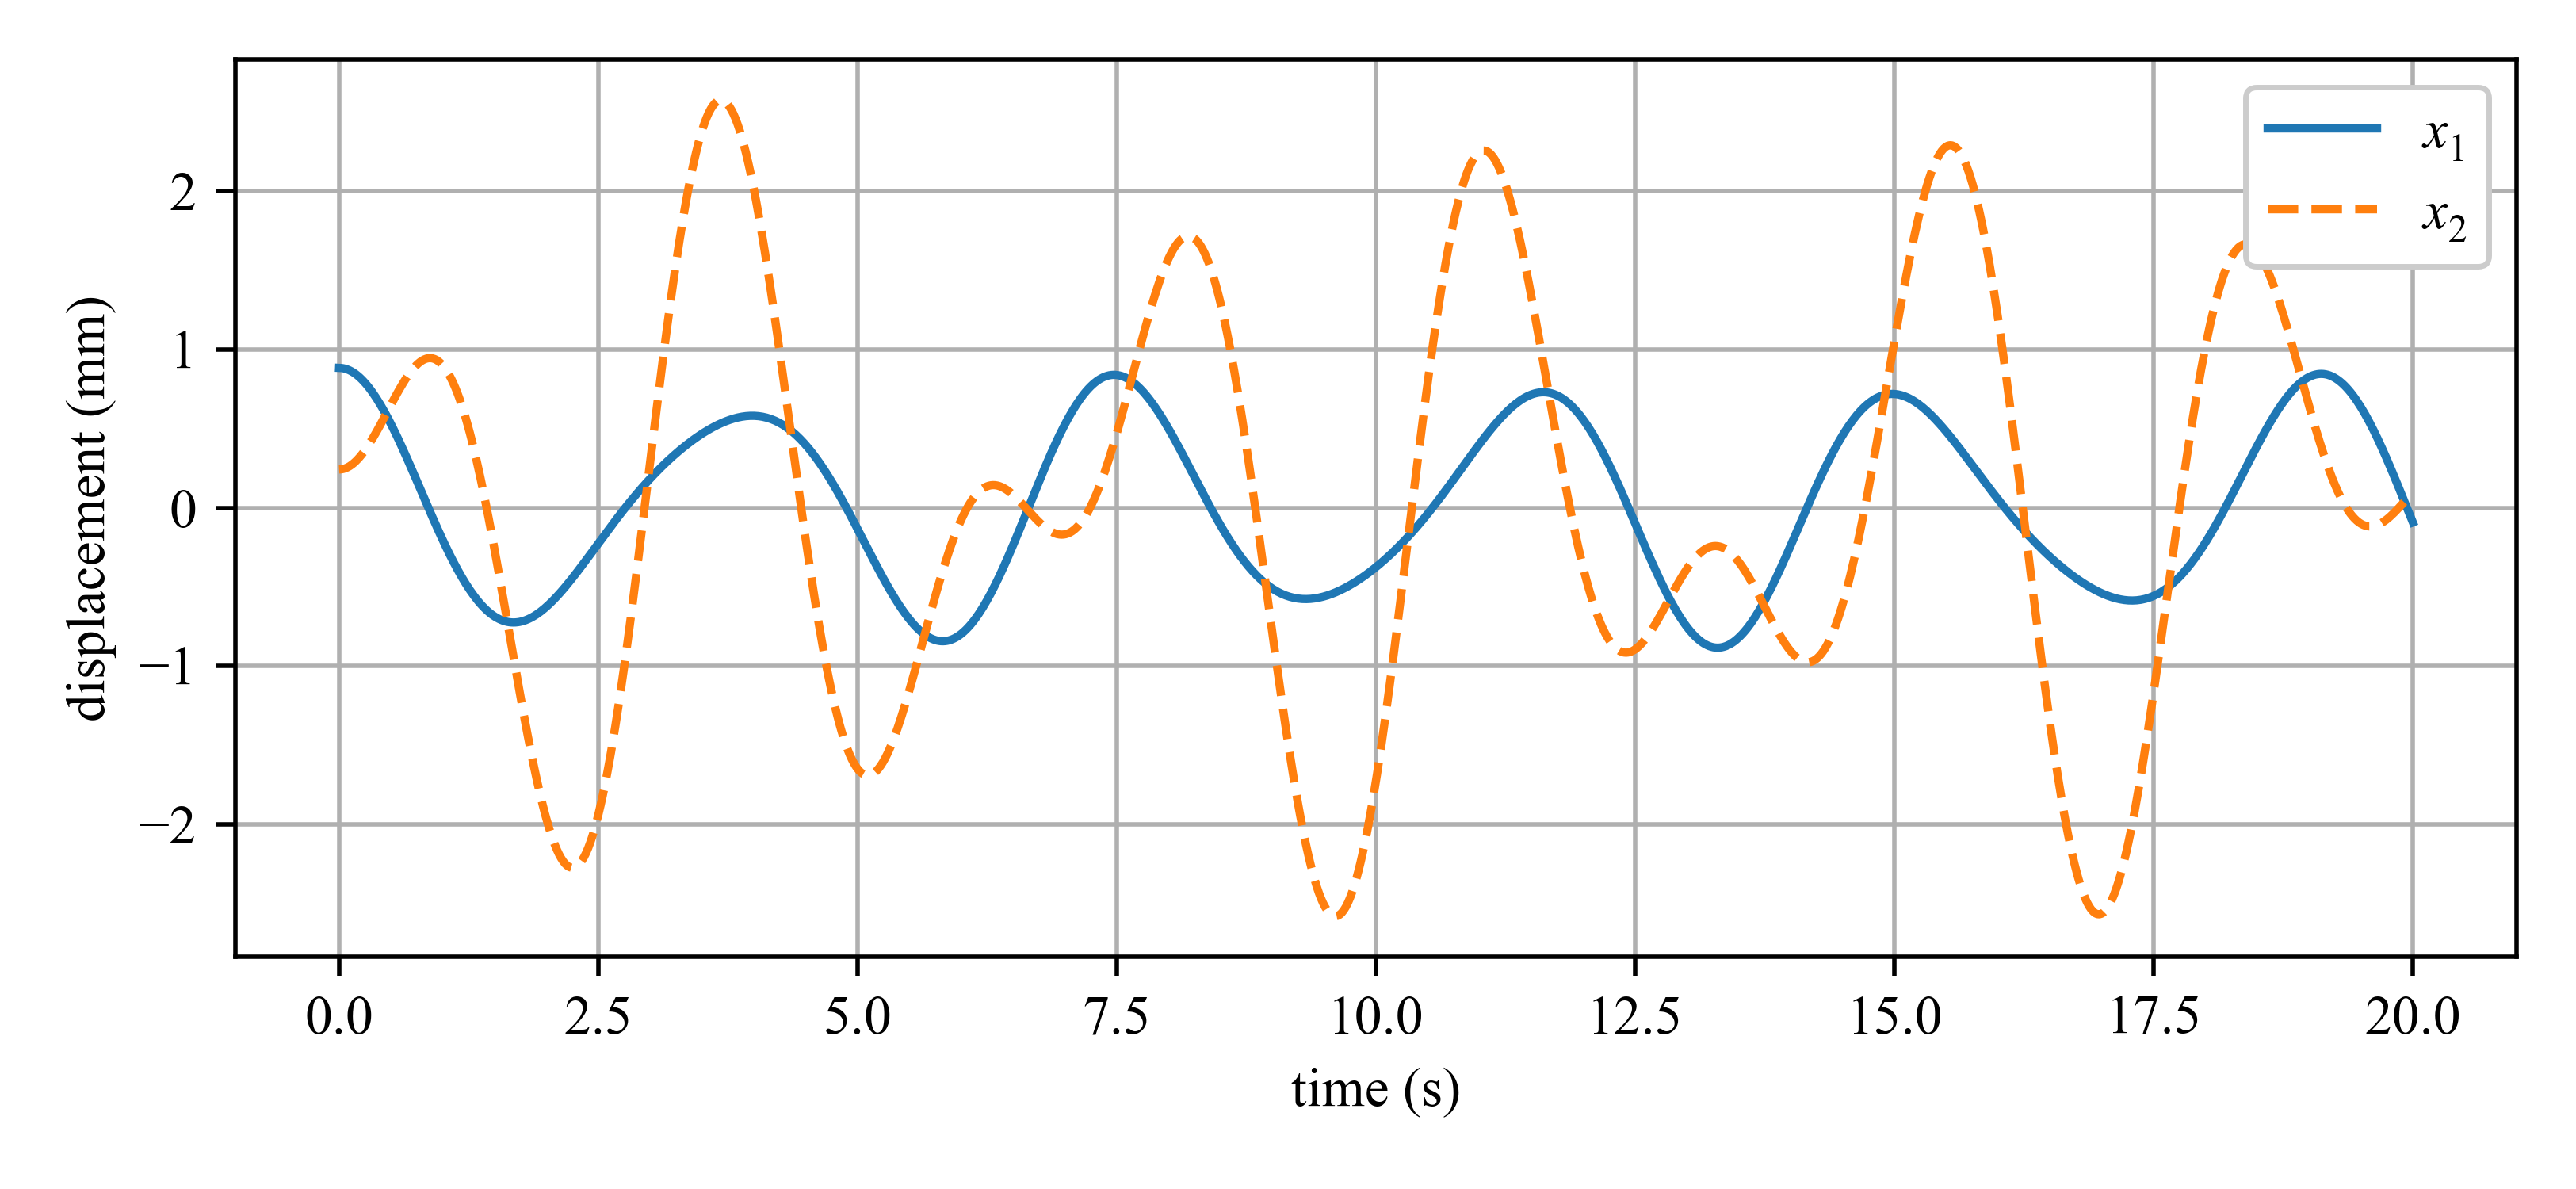
\includegraphics[width=\linewidth]{../figures/modal_analysis_free_vibration.png}
		\caption{Temporal response for the 2-DOF reconstructed using just all the modal coordinates.}
		\label{fig:modal_analysis_free_vibration}
	\end{figure}
	
	Next, the truncated response can be computed by only considering the first mode response for the system (i.e. $\vec{x}(t) = q_1(t) \vec{v}_1$). This is obtained as:
	
	\begin{equation}
	\vec{x}(t) = P\vec{q}_\text{truncated}(t) = \begin{bmatrix} 0.28 & -0.14 \\    0.43  & 0.90 \end{bmatrix}  \begin{bmatrix} 2.85 \cdot \cos (1.65 t) \end{bmatrix}
	\end{equation}
	This is further simplified into:
	\begin{eqnarray}
	x_1(t) = 0.81 \cdot \cos (1.65 t) \\ 
	x_2(t) = 1.24 \cdot \cos (1.65 t) \nonumber
	\end{eqnarray}
	These results are plotted in figure~\ref{fig:modal_analysis_free_vibration_truncated}. Note that this only considers the response of the system that is a function of the first mode. Note that this captures some of the ``general'' idea of the system while missing out on the finer points that the 2$^{\text{nd}}$ mode contributes. 
	
	\begin{figure}[H]
		\centering
		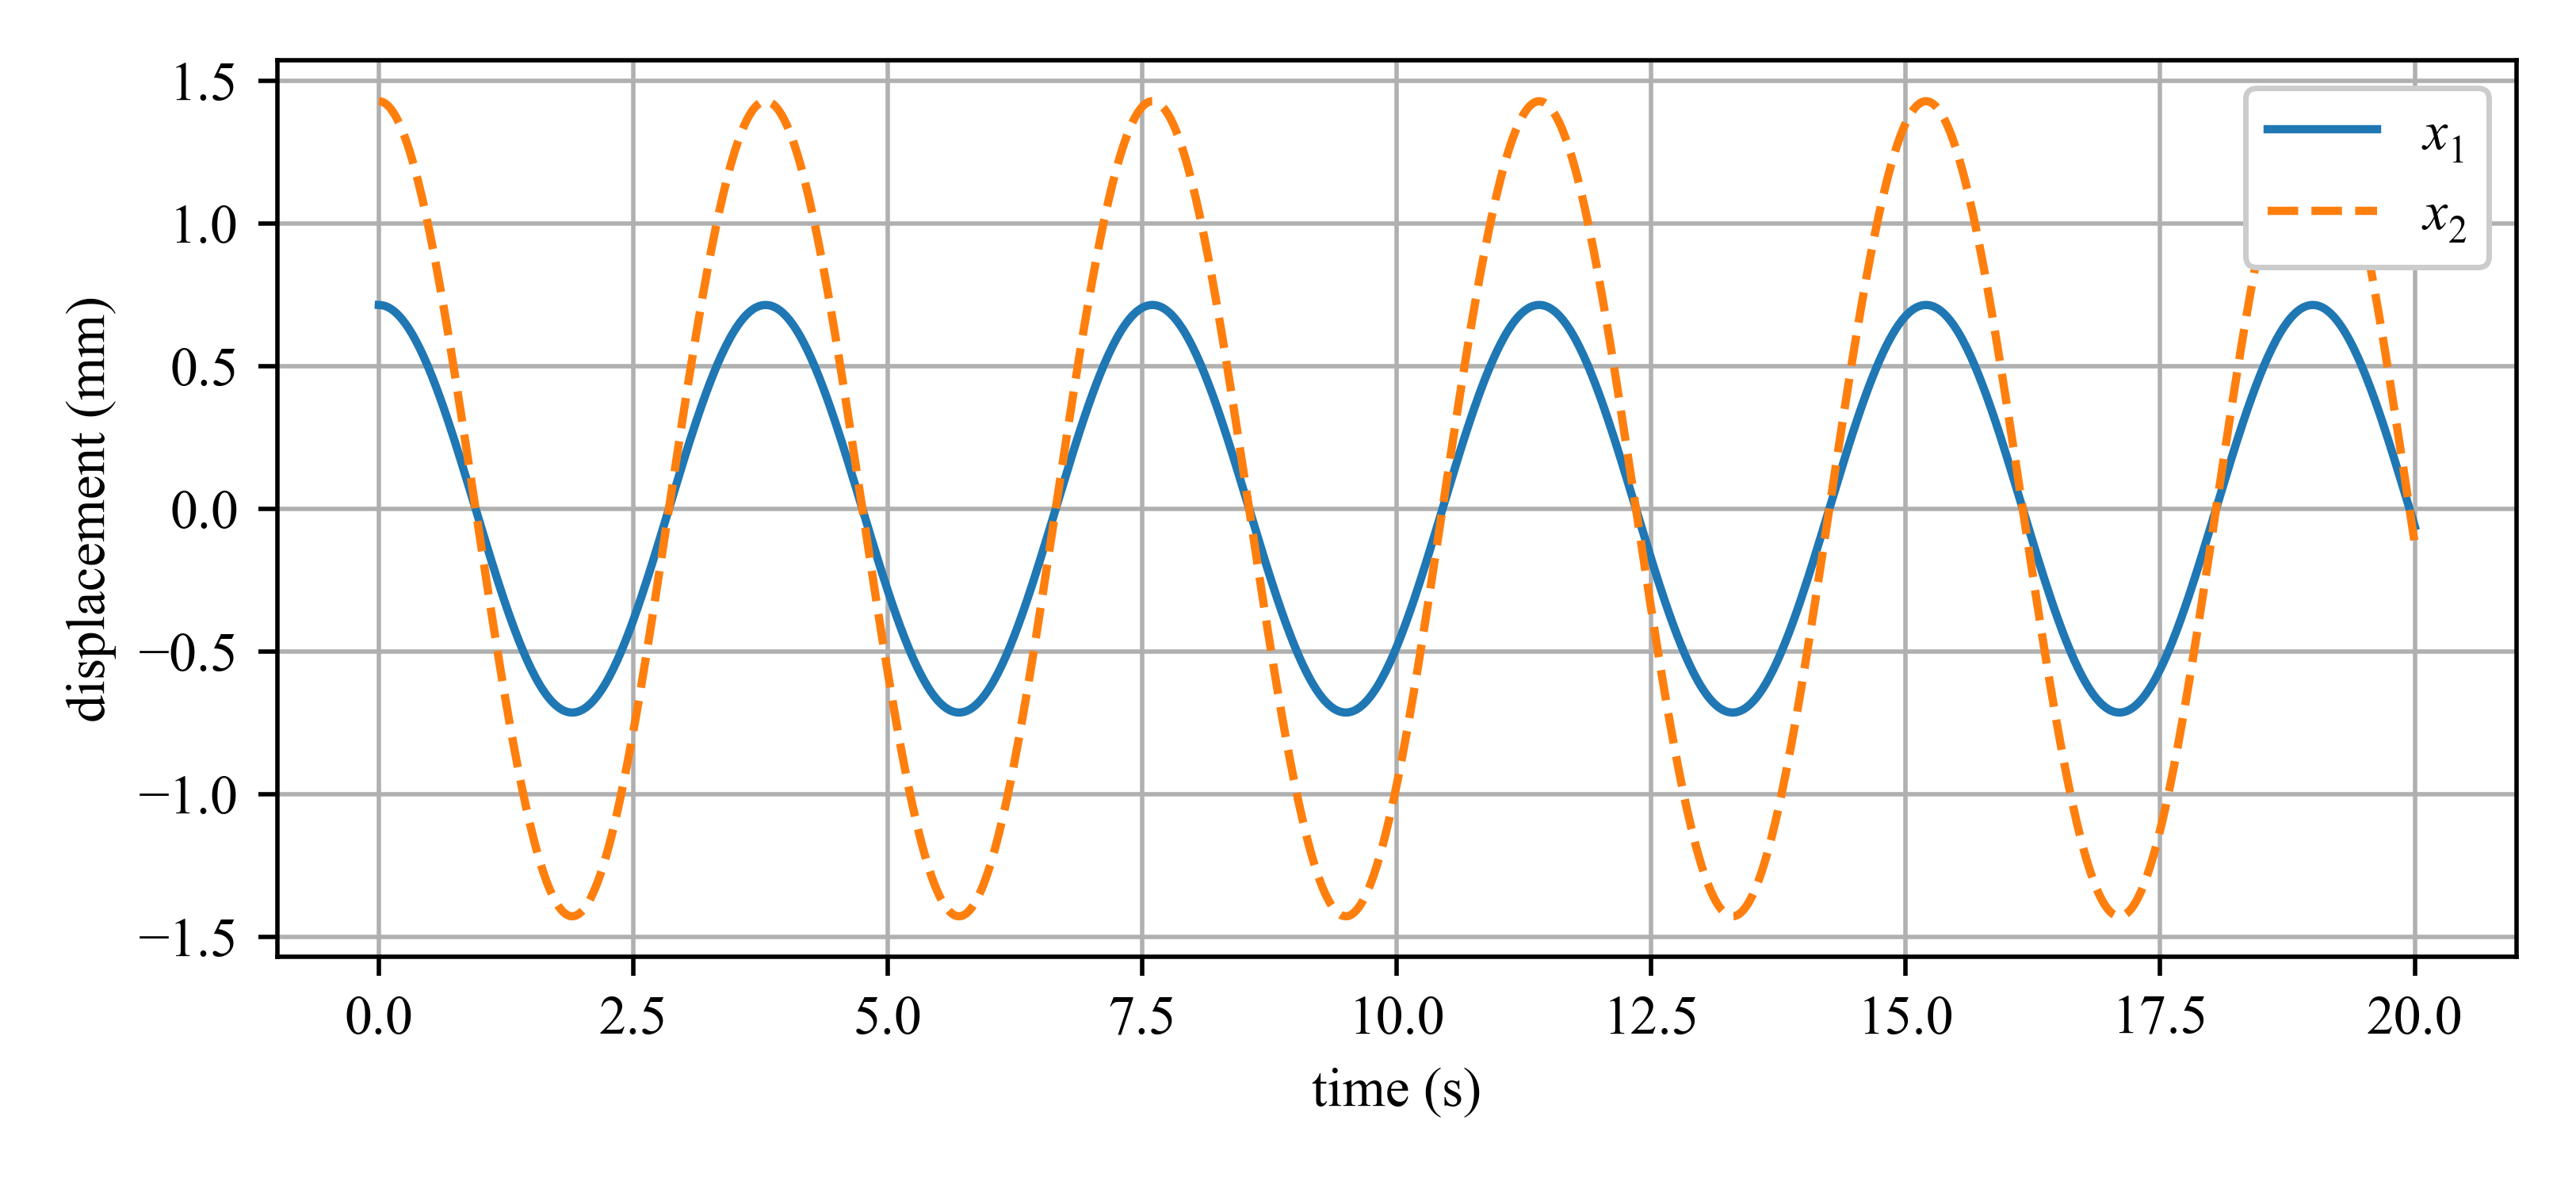
\includegraphics[width=\linewidth]{../figures/modal_analysis_free_vibration_truncated.png}
		\caption{Truncated temporal response for the 2-DOF reconstructed using just the first modal coordinates.}
		\label{fig:modal_analysis_free_vibration_truncated}
	\end{figure}
	
	Lastly, the participation of the two modes can be plotted from the time series response of equation~\ref{eq:participation}.
	
	\begin{figure}[H]
		\centering
		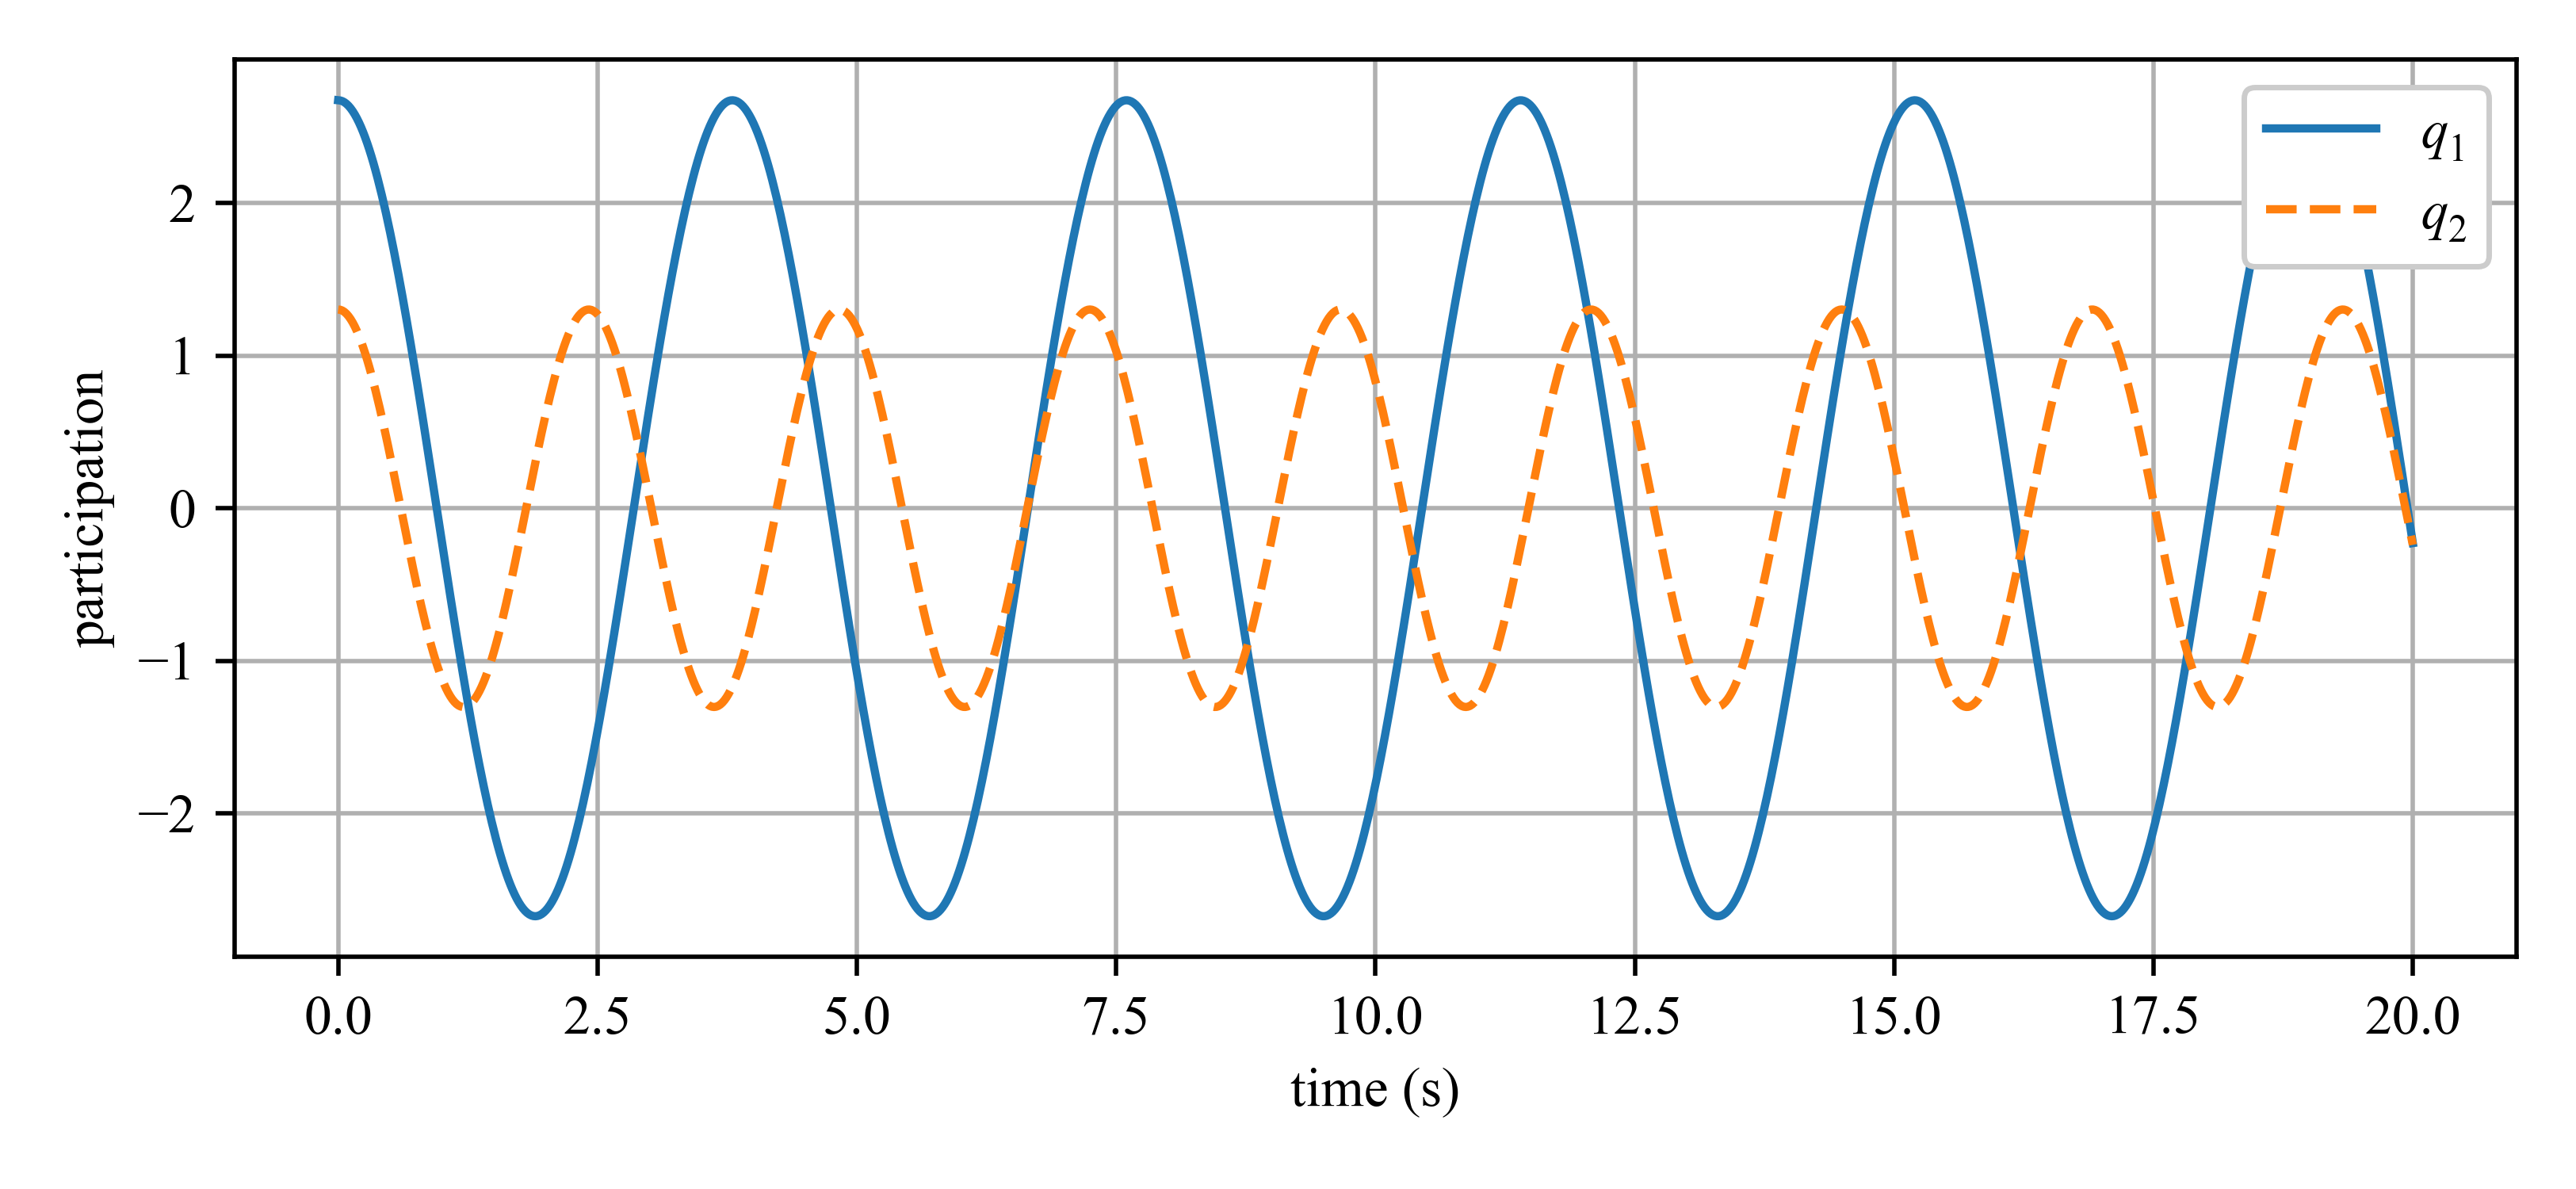
\includegraphics[width=\linewidth]{../figures/modal_analysis_free_participation_factors.png}
		\caption{Modal participation coefficients.}
		\label{fig:modal_analysis_free_participation_factors}
	\end{figure}
	
	
	
	\end{example}
	
		\subsection{Numerical Methods}
		
			Numerical methods can be used to solve the response of multi-degree of freedom system subjected to forced vibrations. While not the most computationally efficient method, the EOM is an ODE that can be solved directly while considering the initial directions to obtain the response of the system. 
			

			

	
	\begin{example}
	\textbf{Directly Solving the ODE of the EOM for a 2-DOF system.} \\

	\noindent Consider the system presented in figure~\ref{fig:2-DOF-spring_mass_dashpot_horizontal_forced_ramp_function}(a) where $m_1$=2~kg, $m_2$=1~kg, $k_1$ = 20~N/m, $k_2$ = 10~N/m, $c_1=0.5$~kg/s, and $c_2=1$~kg/s; initially at rest. $m_1$ is subjected to the ramp and hold load shown in figure~\ref{fig:2-DOF-spring_mass_dashpot_horizontal_forced_ramp_function}(b). 	Using MATLAB, solve the EOM for the temporal response 2-DOF system using a numerical ODE solver.

			\begin{figure}[H]
				\centering
				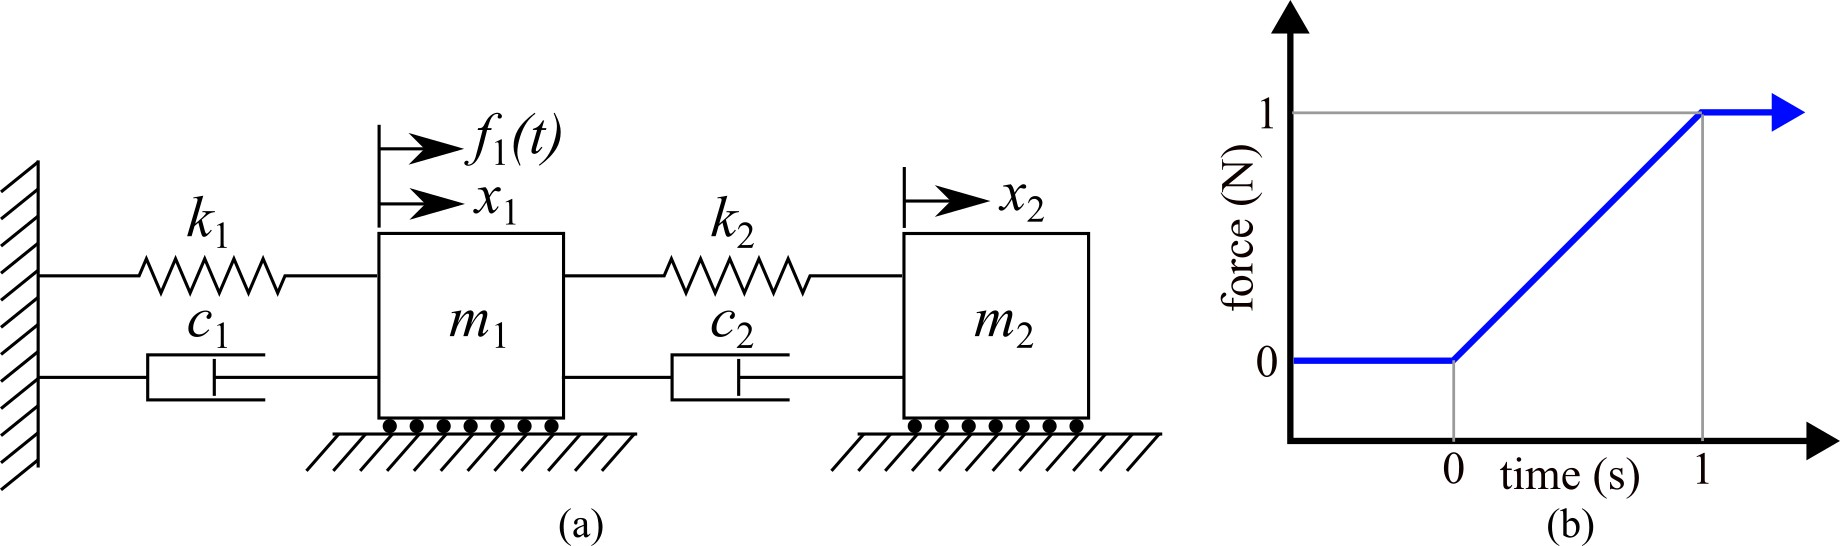
\includegraphics[width=\linewidth]{../figures/2-DOF-spring_mass_dashpot_horizontal_forced_ramp_function}
				\caption{2-DOF system with two masses and two independent confidante systems $x_1$ and $x_2$.}
				\label{fig:2-DOF-spring_mass_dashpot_horizontal_forced_ramp_function}
			\end{figure}
			
			
\noindent \textbf{Solution:} 
	
\noindent Assuming $x_1<x_2$, the matrix form of the system is
	
				\begin{eqnarray}
				  \begin{bmatrix} m_1 & 0  \\  0 & m_2 \end{bmatrix}\begin{bmatrix} \ddot{x_1} \\  \ddot{x_2} \end{bmatrix} + \begin{bmatrix} c_1+c_2 & -c_2  \\  -c_2 & c_2 \end{bmatrix}\begin{bmatrix} \dot{x}_1 \\  \dot{x}_2 \end{bmatrix} + \begin{bmatrix} k_1+k_2 & -k_2  \\  -k_2 & k_2 \end{bmatrix}\begin{bmatrix} x_1 \\  x_2 \end{bmatrix}  = \begin{bmatrix} \ R(t) \\  0 \end{bmatrix}
				\end{eqnarray} \\
where $R(t)$ is the piecewise ramp function shown in figure~\ref{fig:2-DOF-spring_mass_dashpot_horizontal_forced_ramp_function}(b). This expression can be re-arranged to:				
\begin{equation}
\ddot{\vec{x}} = M^{-1}(F_t - C \cdot \dot{\vec{x}} -K \cdot \vec{x})
\end{equation}
which is the format required by MATLAB's \texttt{ode45} solver. Thereafter, the code in listings~\ref{lst:code} and \ref{lst:functions} can be used to develop the results shown in figure~\ref{fig:ODE_results-2-DOF}. 


			


	

\lstset{%
caption={MATLAB code for solving the EOM of the two-degree-of-freedom system.},
label={lst:code},
basicstyle=\ttfamily\footnotesize\bfseries,
frame=tb,
}
\begin{lstlisting}
% Time span for simulation
tspan = [0, 10]; % Start time and end time

% Initial conditions [x1, x1', x2, x2']
initial_conditions = [0, 0, 0, 0];

% Use ode45 to solve the system of ODEs
[t, y] = ode45(@equations_of_motion, tspan, initial_conditions);

% Extract displacements of masses
x1 = y(:, 1);
x2 = y(:, 3);
\end{lstlisting}
	
	
\lstset{%
caption={Functions for Matlab code.},
label={lst:functions},
basicstyle=\ttfamily\footnotesize\bfseries,
frame=tb,
}
\begin{lstlisting}
% Equations of motion for the system
function [dydt] = equations_of_motion(t, y)

	% Setup the system parameters
	m1=2; m2=1; k1=20; k2=10; c1=0.5; c2=1;
	
	% Build the Mass, Damping, and Stiffnes matrices 
	M = [m1, 0; 0, m2];
	C = [c1 + c2, -c2; -c2, c2];
	K = [k1 + k2, -k2; -k2, k2];
	
	% Unpack the state variables
	x = y(1:2);
	x_dot = y(3:4);
	
	% Get the force excitation vector at time t
	F_t = force_excitation_vector(t);
	
	% Equations of motion
	x_dotdot = inv(M) * (F_t - C * x_dot - K * x);
	
	% Pack the derivatives into the output vector dydt
	dydt = [x_dot; x_dotdot];
end

% Define the force excitation vector F(t)
function F_t = force_excitation_vector(t)
	
	if t<1 % Ramp load from 0 to 1 second 
	    f1_t = t;
	else % constant load after 1 second 
	    f1_t=1;
	end
	
	% Force vector, with no load on f2
	F_t = [f1_t; 0]; 

end
\end{lstlisting}
	
	
\begin{figure}[H]
	\centering
	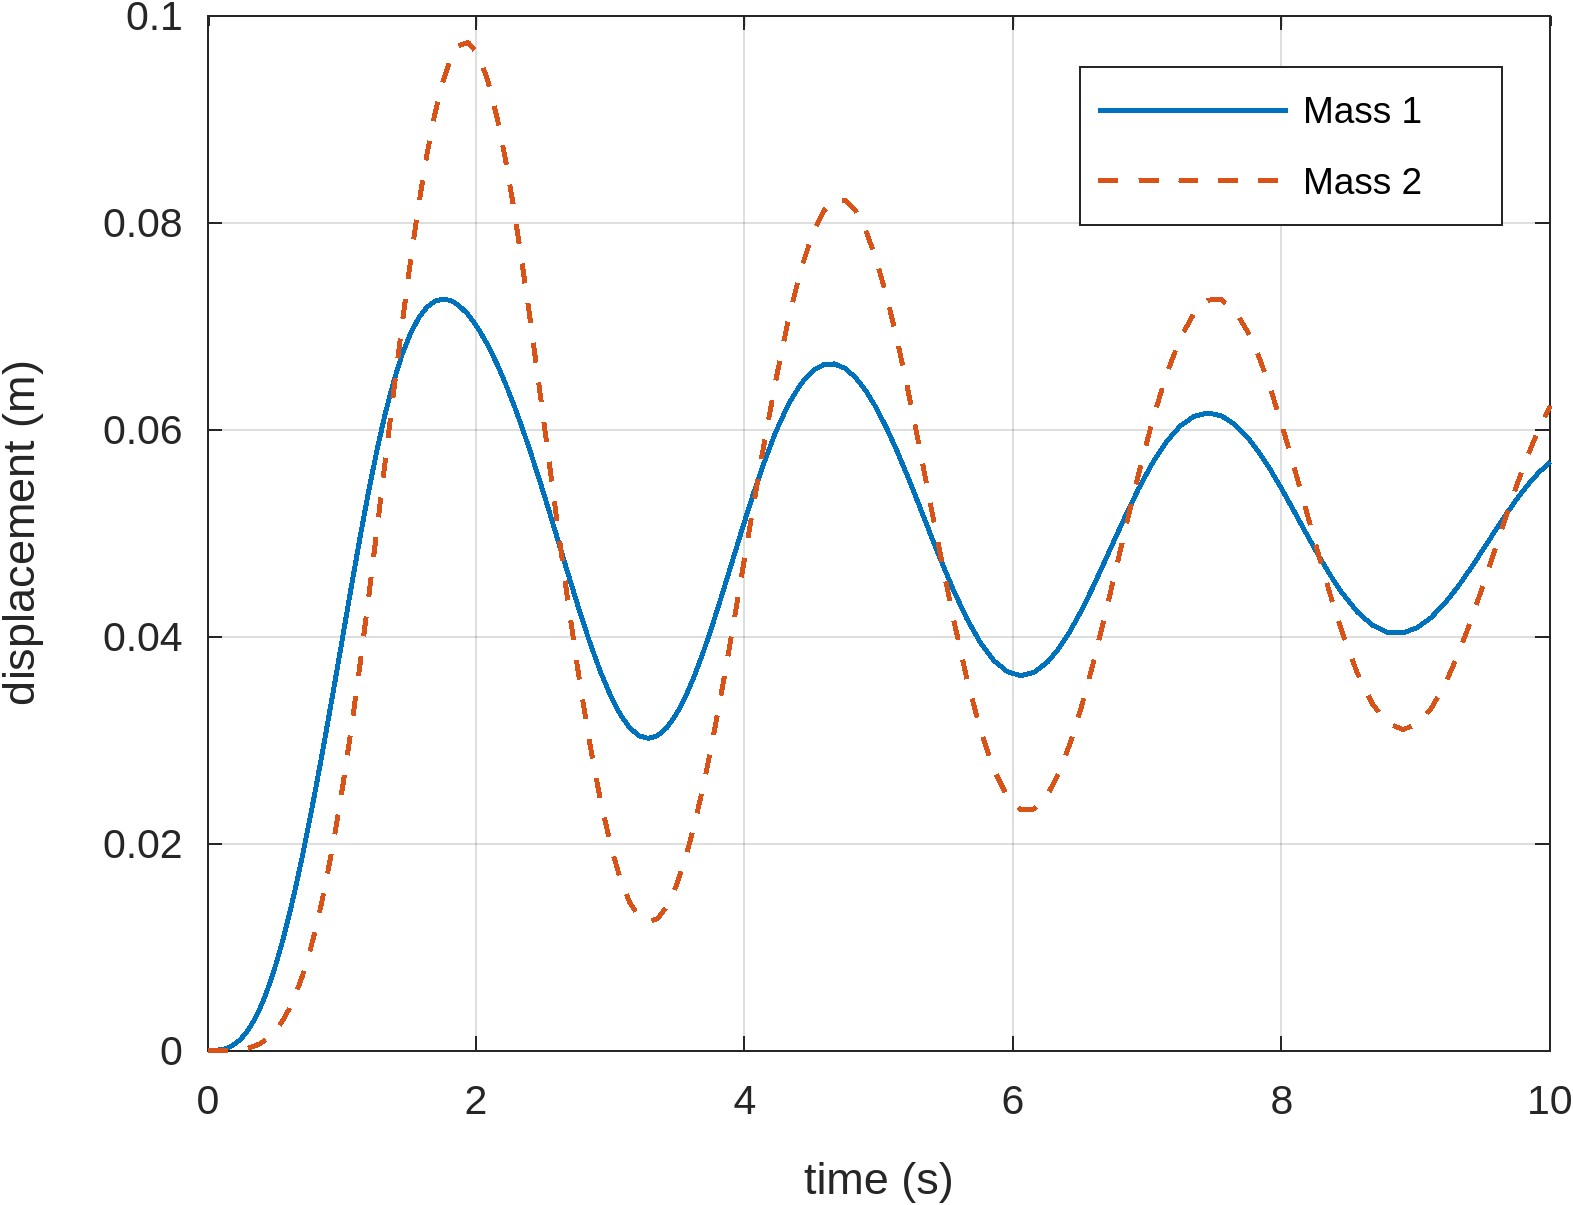
\includegraphics[width=4.25in]{../figures/ODE_results-2-DOF}
	\caption{Displacement response of the 2-DOF system.}
	\label{fig:ODE_results-2-DOF}
\end{figure}
				
	\end{example}
				

\end{document}














